\documentclass[b5paper]{book}
\usepackage{ctex}
\usepackage[margin=0.8in]{geometry}
\geometry{top=2.5cm}
\usepackage{amsmath}
\usepackage{caption}
\usepackage{indentfirst}
\usepackage{graphicx}
\usepackage{subfigure}
\usepackage{amssymb}
\usepackage{cuted}
\usepackage{color}
\usepackage[dvipsnames]{xcolor}
\usepackage{fancyhdr}
\usepackage{xeCJK}
\usepackage{titlesec}
\usepackage{float}
\definecolor{titleBlue}{RGB}{30,59,150}
\titleformat{\chapter}[block]{\huge\bfseries\color{titleBlue}}{第 \thechapter 章}{1em}{}
\titleformat{\section}[block]{\Large\bfseries\color{titleBlue}}{\thesection}{1em}{}
\titleformat{\subsection}[block]{\large\bfseries\color{titleBlue}}{\thesubsection}{1em}{}
\titlespacing*{\section} {0pt}{10pt}{0pt}
% \renewcommand{\chaptermark}[1]{\markboth{第\,\thechapter\,章\quad #1}{}}

\pagestyle{fancy}
\renewcommand{\chaptermark}[1]{\markboth{\CJKfamily{hei} \color{titleBlue}{第 \thechapter 章\quad #1} }{}}
\renewcommand{\sectionmark}[1]{\markright{\CJKfamily{hei} \color{titleBlue}  \thesection \quad #1}{}}

\fancyhead{} % clear all fields
\fancyhead[LO]{\CJKfamily{hei} \bfseries \color{titleBlue}{\rightmark}}
\fancyhead[RO]{\CJKfamily{hei} \bfseries \color{titleBlue}  \thepage}
\fancyhead[LE]{\CJKfamily{hei} \bfseries \color{titleBlue}  \thepage}
\fancyhead[RE]{\CJKfamily{hei} \bfseries \color{titleBlue}{\leftmark}}

\fancyfoot{}

\renewcommand{\headrulewidth}{0pt}
\renewcommand{\footrulewidth}{0pt}


\setlength{\parindent}{2em}
\renewcommand {\thetable} {\thechapter{}.\arabic{table}}
\renewcommand {\thefigure} {\thechapter{}.\arabic{figure}}
\numberwithin{equation}{chapter}

\newcommand {\bx} {\boldsymbol{\mathrm{x}}}
\newcommand {\bw} {\boldsymbol{\mathrm{w}}}
\newcommand {\sfx} {\boldsymbol{\mathsf{x}}}
\newcommand {\sft} {\boldsymbol{\mathsf{t}}}
\newcommand {\sfy} {\boldsymbol{\mathsf{y}}}
\newcommand {\rmT} {\mathrm{T}}
\newcommand {\rmd} {\mathrm{d}}
\newcommand {\bfMu} {\boldsymbol{\mu}}
\newcommand {\bfAl} {\boldsymbol{\alpha}}
\newcommand {\bfSigma} {\boldsymbol{\Sigma}}
\newcommand {\bfLambda} {\boldsymbol{\Lambda}}
\newcommand {\bfPhi} {\boldsymbol{\Phi}}
\newcommand {\bfphi} {\boldsymbol{\phi}}
\newcommand {\bfeta} {\boldsymbol{\eta}}
\newcommand {\calD} {\mathcal{D}}
\newcommand {\calN} {\mathcal{N}}
\newcommand {\calR} {\mathcal{R}}
\newcommand {\insertline} {\noindent{\color{red} \rule[5pt]{\textwidth}{0.1em}}}

\author{张括嘉 \\ 东北大学机器人科学与工程学院}

\begin{document}
\title{Pattern Recognition and Machine Learning 中文版}
\date{}
% \maketitle
	\chapter{绪 \quad 论}
	\noindent\rule[0.25\baselineskip]{\textwidth}{1pt}
	\renewcommand {\thetable} {\thechapter{}.\arabic{table}}
	\renewcommand {\thefigure} {\thechapter{}.\arabic{figure}}
	
	\chapter{概率分布}
	\noindent\rule[0.25\baselineskip]{\textwidth}{1pt}
	\renewcommand {\thetable} {\thechapter{}.\arabic{table}}
	\renewcommand {\thefigure} {\thechapter{}.\arabic{figure}}
	
	\chapter{线性回归模型}
	\noindent\rule[0.25\baselineskip]{\textwidth}{1pt}
	\renewcommand {\thetable} {\thechapter{}.\arabic{table}}
	\renewcommand {\thefigure} {\thechapter{}.\arabic{figure}}
	\textnormal{
	\indent 到目前为止,这本书主要讨论的内容还主要集中在非监督学习上,之前讨论的密度估计问题和数据聚类问题都属于这一类。现在我们将目光转向监督学习,从回归问题开始监督学习的相关讨论。回归问题的目的,是在给定了$D$维输入变量$\bx$的情况下,对一个或多个连续目标变量$t$进行预测。在第1章中我们已经见过这样的问题,也就是多项式曲线拟合问题。多项式是一个广泛的函数类型中的特例,这种函数类型称为线性回归模型。线性回归模型共同的性质是,它们都是可调参数的线性函数,我们将在本章节中重点研究它们。最简单的线性模型同样也是输入变量的线性函数。不过我们也可以通过将输入变量的非线性函数进行线性组合,从而得到更多的函数类型,这些非线性函数称为基底函数(basis function)。这些模型都是参数的线性函数,同时还是关于输入变量的非线性函数,这样的特点使它们具有很多简单有效的性质。\\
	\indent 我们要做的工作是,在给定了一个训练集$\{\bx_n\}$和对应的目标值$\{t_n\}$(其中共有$N$组数据,$n=1,...,N$)的情况下,对一个新的输入量$\bx$预测$t$的值。最简单的方法是直接构建一个适当的函数$y(\bx)$,并认为在$\bx$处的函数值就是预测的$t$值。从概率的角度来说,一般地,我们要对预测分布$p(t|\bx)$建模,因为预测分布可以表达每一个$\bx$所对应的$t$的不确定性。根据这个条件分布,我们可以通过将适当的损失函数进行最小化,从而对任何的$\bx$做出预测$t$。在第1.5.5节中曾经讨论过,对于实值变量,通常会选择平方损失函数,这个损失函数的最优解是在$t$的条件期望处取得的。\\
	\indent 尽管线性模型在模式识别的实际应用中具有明显的局限性,尤其是在应对高维的输入空间时显得力不从心,但它们具备的性质实在是太好了,而且是一些后文中更加实用的模型的基础,所以线性模型还是很值得讨论一下的。
	}
	\section{线性基底函数模型}
	\insertline
	\textnormal{
	\indent 最简单的线性回归模型是输入变量的线性组合
	\begin{equation}
		y(\bx,\bw) = w_0+w_1x_1+...+w_D x_D
	\end{equation}
	其中$\bx=(x_1,...,x_D)^{\rmT}$。这个模型通常称为线性回归函数。这个模型最重要的性质是,它是关于参数$w_0,...,w_D$的线性函数。不过还有个特殊之处,它同时还是关于输入变量$x_i$的线性函数,这就是这个模型最明显的短板。所以我们将这个类型的模型进行扩展成输入变量非线性函数的线性组合,也就是
	\begin{equation}
		y(\bx,\bw)=w_0 + \sum_{j=1}^{M-1}w_j \phi_j(\bx)
	\end{equation}
	其中$\phi_j(\bx)$称为基底函数(basis function)。设参数$j$的最大值为$M-1$可以使参数的总数量为$M$,表达起来更加方便一些。\\
	\indent 参数$w_0$称为偏差参数(bias parameter),是控制全部数据发生固定偏移的参数(注意不要和统计学中的"bias"搞混了)。通常来说把它表示为一个附加的“基底函数”$\phi_0(\bx)=1$要更加方便一些,于是
	\begin{equation}
		y(\bx,\bw)=\sum_{j=0}^{M-1}w_j \phi_j(\bx) = \bw^{\rmT} \bfphi(\bx)
	\end{equation}
	其中$\bw=(w_0,...,w_{M-1})$,$\bfphi = (\phi_0,\phi_{M-1})$。在模式识别的很多实际应用中,我们会对原始的数据进行某些形式的预处理,或者称为特征提取。如果将原始变量表示为向量$\bx$,那么特征就可以表示为基底函数$\{\phi_j(\bx)\}$。\\
	\indent 利用非线性基底函数,使得函数$y(\bx,\bw)$成为输入向量$\bx$的非线性函数。但(3.2)这样的函数仍然称为线性模型,因为它们是关于$\bw$的线性函数。正是这种关于参数的线性性质,使得线性模型的分析变得非常简单。但是这个性质所导致的问题也比较令人难受,具体内容将在第3.6节中进行讨论。\\
	\indent 第1章中讨论的多项式回归问题是线性模型的典型案例,在这个问题中仅有一个输入变量$x$,基底函数是$x$的幂函数,于是$\phi_j(x)=x^j$。多项式基底函数的一大缺陷在于,它们都是输入变量的全局函数,所以在局部的调整会影响到全局。可以将输入控件进行划分,并在每个区域内分别进行多项式拟合,从而解决这个问题,这样得到的模型称为样条函数(spline functions, Hastie et al., 2001)。\\
	\indent 此外,基底函数还有很多的选择。比如,
	\begin{equation}
		\phi_j(x)=\exp\left\{-\frac{(x-\mu_j)^2}{2s^2}\right\}
	\end{equation}
	其中$\mu_j$控制了基底函数在输入控件中的位置,参数$s$控制了基底函数的空间尺度。这种基底函数通常称为高斯基底函数,尽管这些函数并没有明确的概率解释,而且归一化是完全不可能的,因为基底函数还要乘上一个参数$w_j$。\\
	\indent 另一种常见的基底函数称为sigmoid基底函数,
	\begin{equation}
		\phi_j(x)=\sigma\left(\frac{x-\mu_j}{s}\right)
	\end{equation}
	其中$\sigma(a)$为对数几率sigmoid函数(logistic sigmoid function),
	\begin{equation}
		\sigma(a)=\frac{1}{1+\exp(-a)}
	\end{equation}
	等价地,我们也可以利用"tanh"函数,因为它与对数几率函数是有关联的,$\tanh (a) = 2\sigma(2a)-1$,所以一般地,对数几率函数的线性组合等价于$\tanh$函数的线性组合。这些基底函数的图像如图3.1所示。
	\begin{figure}[ht]
	\centering
		\begin{minipage}[t]{0.3\linewidth}
		\centering
		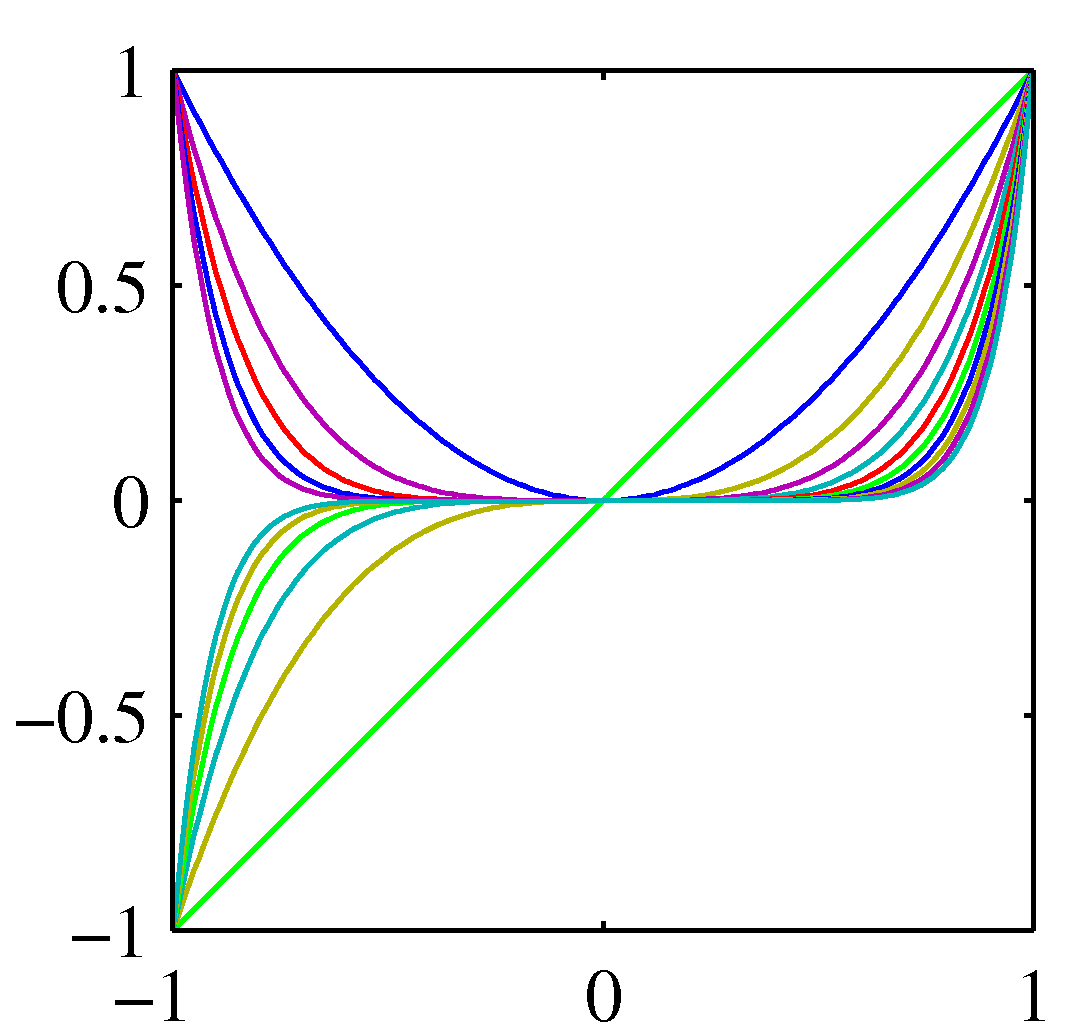
\includegraphics[scale=0.8]{Images/3-1a.png}
		\label{fig:3-1a}
		\end{minipage}
		\begin{minipage}[t]{0.3\linewidth}
		\centering
		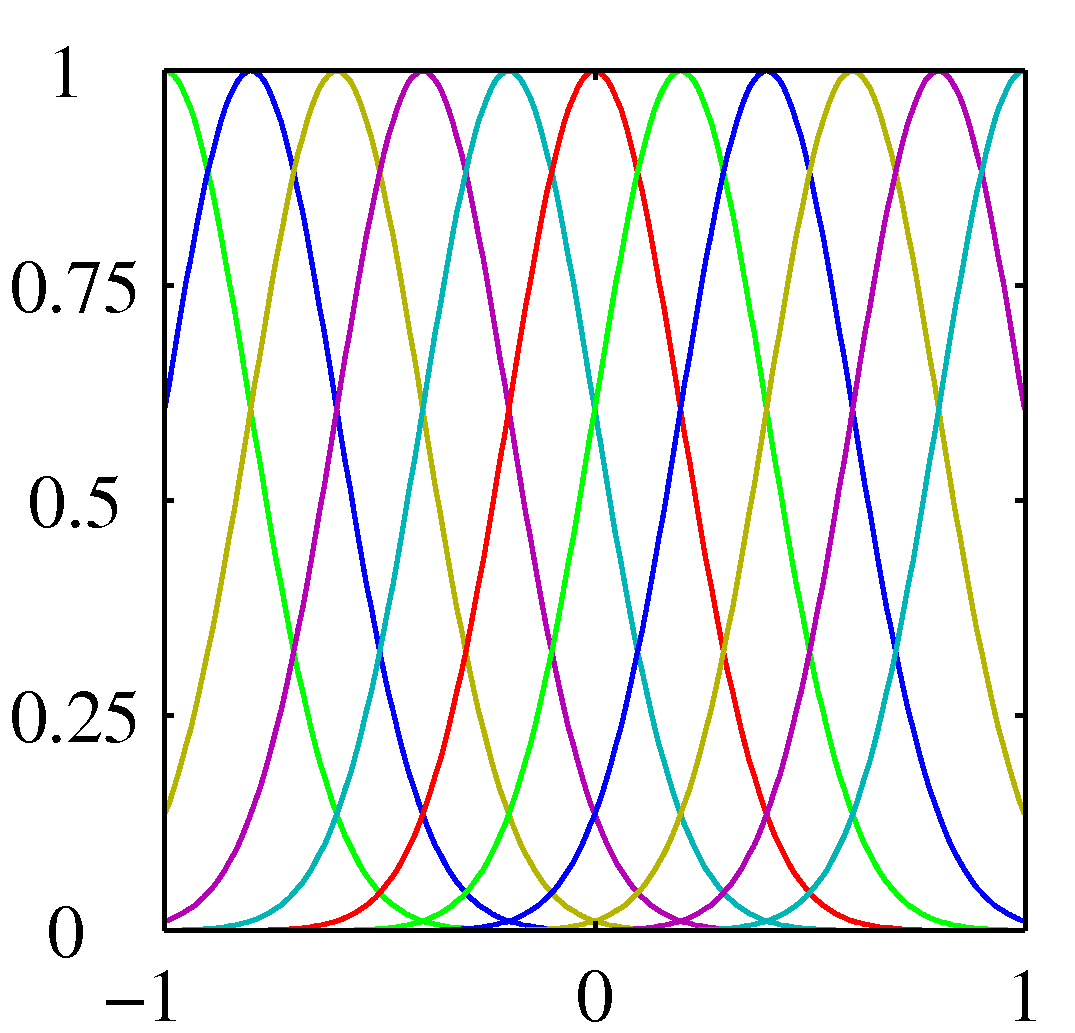
\includegraphics[scale=0.8]{Images/3-1b.png}
		\label{fig:3-1b}
		\end{minipage}
		\begin{minipage}[t]{0.3\linewidth}
		\centering
		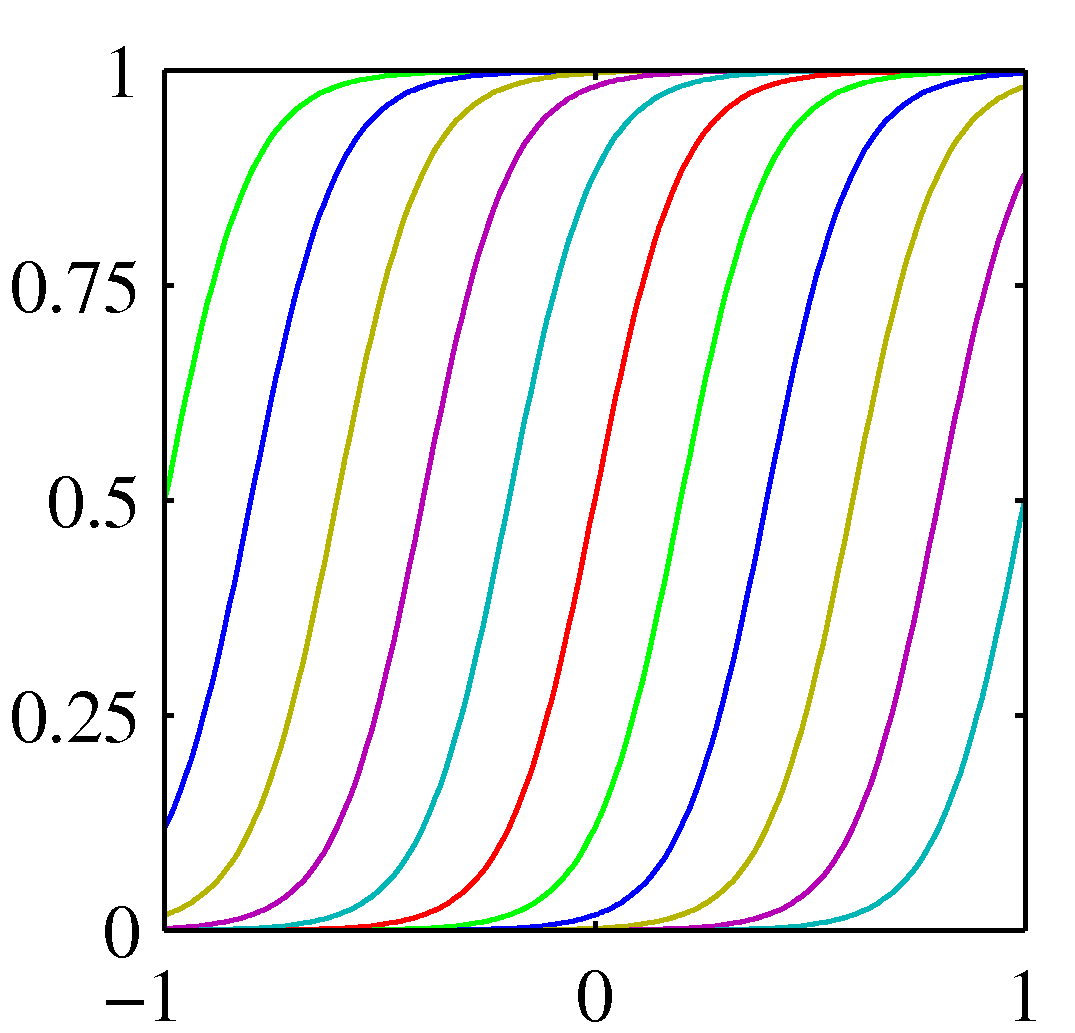
\includegraphics[scale=0.8]{Images/3-1c.png}
		\label{fig:3-1c}
		\end{minipage}
		\captionsetup{font={small}}
		\caption{基底函数示例,从左至右分别为多项式基底函数,高斯基底函数(3.4)和sigmoid基底函数(3.5)。}
	\end{figure}
	\\
	\indent 还有另外一种基底函数称为Fourier基底函数,它可以展开为正弦函数。每个基底函数都代表一个特定的频率,并且在空间中可以无限延伸。与之不同的是,位于输入空间的有限区域内的基底函数必然包含了不同空间频率的频谱。在很多信号处理的实际应用中,需要研究位于空间和频率上的基底函数都是有必要的,于是产生了小波这一类型的函数。为了简化问题,它们往往被定义成正交的。当输入变量存在于规则的点阵中,比如在处理时间序列中的连续时间点,或者图像中的像素时,小波是最适用的。关于小波的具体内容可以参考Ogden (1997), Mallat (1999)和Vidakovic (1999)。\\
	\indent 不过,本章节主要研究的内容与基底函数的选择无关,所以在讨论的过程中并不会指明采用了哪一种基底函数,除非要进行数值计算。实际上,我们的讨论中基本都会使用$\bfphi(\bx)=\bx$作为基底函数。此外,为了让符号变得简洁一些,我们会主要针对单一目标变量$t$展开讨论,不过在第3.1.5节会简单研究一下如何处理多个目标变量的情况。
	}
	\subsection{最大似然与最小二乘法}
	\textnormal{
	在第1章中,我们通过将平方和误差函数进行最小化来拟合多项式函数。我们同时也证明了这个误差函数就是在高斯噪声模型下的最大似然解。让我们再次把目光转向这个问题,并研究求解它的最小二乘法,并研究最小二乘法与最大似然之间的关系。\\
	\indent 和以前一样,我们假设目标变量$t$是由函数$y(\bx,\bw)$加上高斯噪声得到的:
	\begin{equation}
		t=y(\bx,\bw)+\epsilon
	\end{equation}
	其中$\epsilon$是均值为0,精度(逆方差)为$\beta$的高斯随机变量。于是
	\begin{equation}
		p(t|\bx,\bw,\beta)=\calN(t|y(\bx,\bw),\beta^{-1})
	\end{equation}
	回想一下,如果我们构造出平方损失函数,那么对于任意的$\bx$,做出的预测将是目标变量的条件均值。\textcolor{red}{\textbf{——第1.5.5节}}\ 对于高斯条件分布(3.8),条件均值为
	\begin{equation}
		\mathbb{E}[t|\bx]=\int tp(t|\bx)\ \rmd t = y(\bx,\bw)
	\end{equation}
	需要注意的是,将噪声视为高斯噪声的假设隐含着一个含义,那就是给定$\bx$的条件下$t$的条件分布是单峰值的,这可能会在一些应用中出现问题。有一种构造出多峰值条件分布的方法是混合条件高斯分布,这个问题将在第14.5.1节中详细讨论。\\
	\indent 现在来研究一下数据集里的输入量$\mathbf{X}=\{\bx_1,...,\bx_N\}$和它们对应的目标值$t_1,...,t_N$。我们将目标值$\{t_n\}$合并表示为列向量$\sft$,这里要与多元变量$\mathrm{t}$区分开,$\sft$表示的是多个一元变量合并在一起的列向量。假设这些数据是从分布(3.8)独立取出的,于是可以写出似然函数的表达式,而似然函数事实上是两个可调参数$\bw$和$\beta$的函数:
	\begin{equation}
		p(\sft|\mathbf{X},\bw,\beta)=\prod_{n=1}^N \calN (t_n|\bw^{\rmT}\bfphi(\bx_n),\beta^{-1})
	\end{equation}
	其中用到了(3.3)。需要注意的是,在回归(或分类)这样的监督学习问题中,我们并不需要对输入变量的分布进行建模。由于$\bx$始终会存在于分布的条件变量中,所以从现在开始我们索性将$p(\sft|\bx,\bw,\beta)$这样的表达中将$\bx$剔除掉,以保证符号的简洁。对似然函数求对数,并利用一元高斯分布的标准形式(1.46),可得
	\begin{equation}
	\begin{split}
		\ln p(\sft|\bw,\beta) &= \sum_{n=1}^N \ln \calN (t_n|\bw^{\rmT} \bfphi(\bx_n),\beta^{-1}) \\
		&= \frac{N}{2} \ln \beta - \frac{N}{2} \ln (2\pi)-\beta E_D(\bw)
	\end{split}
	\end{equation}
	其中的平方和误差函数为
	\begin{equation}
		E_D(\bw) = \frac{1}{2}\sum_{n=1}^N \{t_n - \bw^{\rmT} \bfphi(\bx_n)\}^2
	\end{equation}
	\indent 在写出了似然函数之后,就可以利用最大似然确定$\bw$和$\beta$了。首先考虑关于$\bw$进行最大化。根据第1.2.5节中的内容,带有高斯噪声的线性模型条件分布的似然函数最大化等价于将平方和误差函数$E_D(\bw)$进行最小化。对数似然函数(3.11)的梯度为
	\begin{equation}
		\nabla \ln p(\sft|\bw,\beta) = \beta \sum_{n=1}^N \{t_n - \bw^{\rmT} \bfphi(\bx_n)\} \bfphi(\bx_n)^{\rmT}
	\end{equation}
	令梯度等于0,
	\begin{equation}
		0 = \sum_{n=1}^N t_n \bfphi(\bx_n)^{\rmT} - \bw^{\rmT} \left(\sum_{n=1}^N\bfphi(\bx_n)\bfphi(\bx_n)^{\rmT}\right)
	\end{equation}
	求解这个方程,可得
	\begin{equation}
		\bw_{\mathrm{ML}}=(\bfPhi^{\rmT}\bfPhi)^{-1}\bfPhi^{\rmT}\sft
	\end{equation}
	这就是最小二乘问题中的正规方程(normal equations)。其中的$\bfPhi$是$N \times M$维矩阵,称为设计矩阵(design matrix),其元素为$\Phi_nj = \phi_j(\bx_n)$,于是
	\begin{equation}
		\bfPhi = \left(
		\begin{matrix}
			\phi_0(\bx_1) & \phi_1(\bx_1) & \cdots & \phi_{M-1}(\bx_1) \\
			\phi_0(\bx_2) & \phi_1(\bx_2) & \cdots & \phi_{M-1}(\bx_2) \\
			\vdots & \vdots & \ddots & \vdots \\
			\phi_0(\bx_N) & \phi_1(\bx_N) & \cdots & \phi_{M-1}(\bx_N)
		\end{matrix} \right)
	\end{equation}
	其中,
	\begin{equation}
		\bfPhi^\dagger \equiv (\bfPhi^{\rmT} \bfPhi)^{-1} \bfPhi^{\rmT}
	\end{equation}
	为矩阵$\bfPhi$的Moore-Penrose伪逆(Moore-Penrose pseudo-inverse, Rao and Mitra, 1971; Golub and Van Loan, 1996)。可以将它看成是矩阵的逆在矩阵并非方阵情况下的扩展。实际上,如果$\bfPhi$为方阵且可逆,利用$(\mathbf{AB})^{-1}=\mathbf{B}^{-1} \mathbf{A}^{-1}$,可以看出$\bfPhi^{\dagger} \equiv \bfPhi^{-1}$。\\
	\indent 此时我们可以获得更多的关于偏差参数$w_0$的信息。将偏差参数单独拆分出来,于是误差函数(3.12)就变成了
	\begin{equation}
		E_D(\bw) = \frac{1}{2}\sum_{n=1}^N \{t_n -w_0 -\sum_{j=1}^{M-1}w_j \phi_j (\bx_n)\}^2
	\end{equation}
	关于$w_0$求导并令导数等于0,可以求解出$w_0$
	\begin{equation}
		w_0=\overline{t}-\sum_{j=1}^{M-1}w_j \overline{\phi_j}
	\end{equation}
	其中,
	\begin{equation}
		\overline{t}= \frac{1}{N}\sum_{n=1}^N t_n, \ \overline{\phi_j}=\frac{1}{N}\sum_{n=1}^N \phi_j(\bx_n)
	\end{equation}
	于是偏差$w_0$补偿了目标值(在训练集上的)的平均值与基底函数值的加权平均值之间的差异。\\
	\indent 我们同样可以关于噪声的精度参数$\beta$将对数似然函数(3.11)进行最大化,可以得到
	\begin{equation}
		\frac{1}{\beta_{\mathrm{ML}}}= \frac{1}{N} \sum_{n=1}^N \{t_n - \bw_{\mathrm{ML}}^{\rmT}\bfphi(\bx_n)\}^2
	\end{equation}
	于是可以看出,噪声精度的倒数是由回归函数与目标值之间残差的方差给出的。
	}
	\subsection{最小二乘法的几何意义}
	\textnormal{
	现在我们研究一下最小二乘法的几何意义。假想一个$N$维的空间,其坐标轴为$t_n$,那么$\sft = (t_1,...,t_N)^{\rmT}$为该空间中的向量。在$N$个数据点处所估计的基底函数$\phi_j(\bx_n)$也同样可以表示为该空间中的向量$\boldsymbol{\varphi}_j$,如图3.2所示。需要注意的是,$\boldsymbol{\varphi}_j$对应的是$\bfPhi$的第$j$列,而$\bfphi(\bx_n)$表示的是$\bfPhi$的第$n$行。如果基底函数的数量$M$小于数据点的数量$N$,那么这$M$个向量$\boldsymbol{\varphi}_j (\bx_n)$将可以展开成$M$维的线性子空间$\mathcal{S}$。我们定义$\sfy$为$N$维向量,其元素$y_n = y(\bx_n, \bw)$,$n=1,...,N$。由于$\sfy$是向量$\boldsymbol{\varphi}_j$的任意线性组合,所以它可以存在于$M$维子空间中的任何位置。这样一来,平方和误差(3.12)就等于$\sfy$与$\sft$之间欧氏距离的平方(但相差一个因子1/2)。因此,$\bw$的最小二乘解与位于子空间$\mathcal{S}$中的$\sfy$的选择有关。根据图3.2,似乎这个解就是$\sft$在空间$\mathcal{S}$中的正交投影,而事实正是如此,只需注意到$\sfy$的解是由$\bfPhi \bw_{\mathrm{ML}}$给出的,然后利用正交投影就可以验证这个猜想。\textcolor{red}{\textbf{——习题 3.2}}
	\begin{figure}[ht]
		\centering
		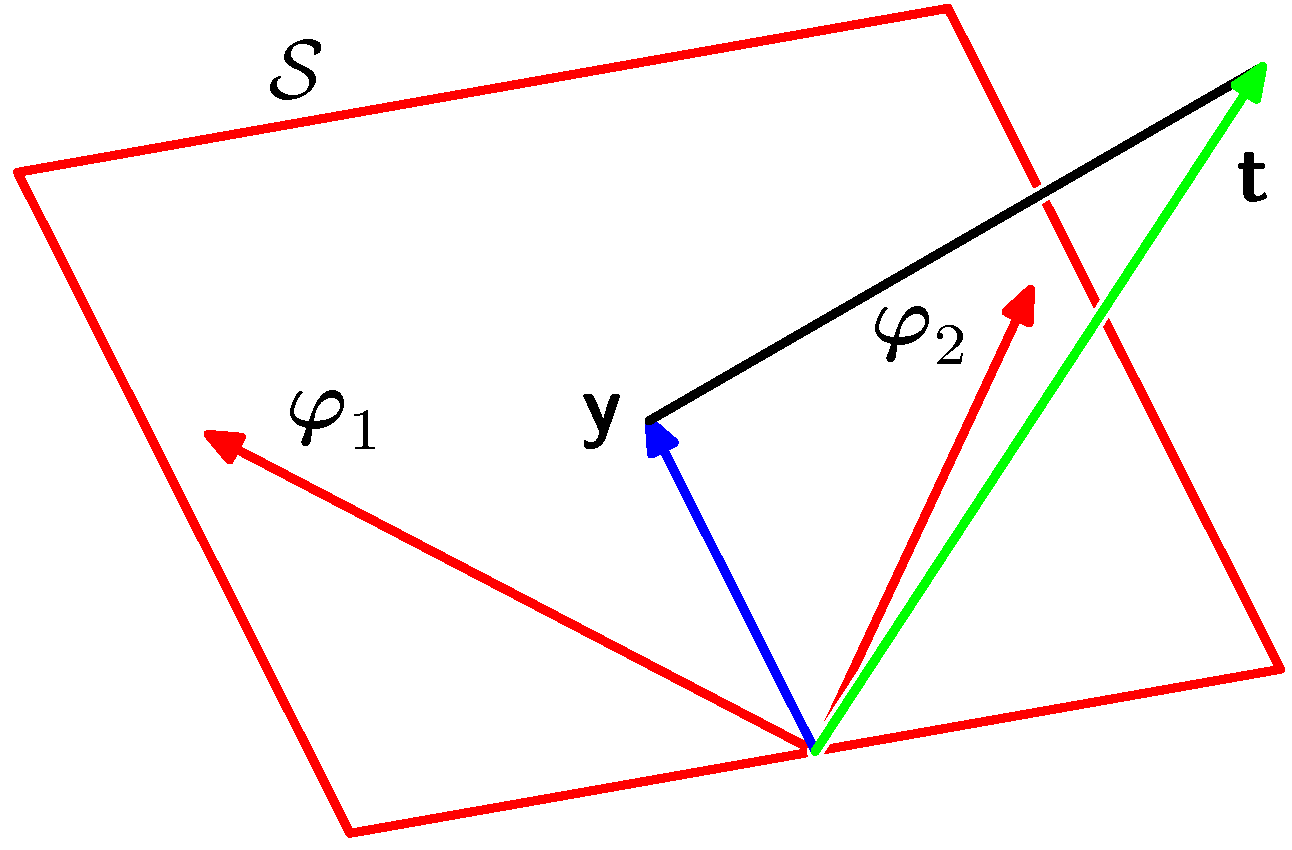
\includegraphics[scale=0.8]{Images/3-2.png}
		\captionsetup{font={small}}
		\caption{分量为$t_1,...,t_N$的$N$维空间中最小二乘解的几何解释。通过寻找数据向量$\sft$在子空间中的正交投影确定最小二乘回归函数,这个子空间是基底函数$\phi_j(\bx)$通过线性组合展开形成的,基底函数$\boldsymbol{\varphi}_j$为长度为$N$,元素为$\phi_j(\bx_n)$的向量。}
		\label{fig:3-2}
	\end{figure}
	\\
	\indent 在实际应用中,如果$\bfPhi^{\rmT} \bfPhi$是接近奇异的,那么直接求解正规方程的话可能会比较困难。特别地,当两个或多个基底向量$\boldsymbol{\varphi}_j$共线或接近共线时,最终得到的参数值可能会比较大。这样的近似简并在真实数据集的处理中并不罕见。计算困难的问题可以通过奇异值分解(SVD, singular value decomposition, Press et al., 1992; Bishop and Nabney, 2008)来解决。需要注意的是,附加的正则项可以确保矩阵的非奇异性,即使是简并的情况下也不例外。
	}
	\subsection{顺序学习}
	\textnormal{
	形如最大似然解(3.15)这样的批处理方法要求一次性处理整个训练集,这样的做法导致的计算压力是非常大的。我们已经在第1章中讨论过,如果数据集是充分大的,那么使用顺序算法,也就是在线算法(on-line algorithm)就是比较划算的了,毕竟每次只需处理一组数据,并时刻更新模型参数。顺序学习也很适合实时应用,毕竟数据是以数据流的形式一点一点流过来的,而且不能等到全部的数据都到达后再做预测。\\
	\indent 我们可以通过如下的随机梯度下降法(stochastic gradient descent),也就是顺序梯度下降法(sequential gradient descent)实现顺序学习算法。假设误差函数$E=\sum_n E_n$是由数据的总和构成的,那么在观测到模式$n$之后,随机梯度下降法会利用如下方式更新参数$\bw$:
	\begin{equation}
		\bw^{(\tau+1)} = \bw^{(\tau)} - \eta \nabla E_n
	\end{equation}
	其中的$\tau$为迭代的循环变量,$\eta$为学习率参数。很快我们会提及$\eta$的选取方法。参数$\bw$的值可以初始化为$\bw^{(0)}$。对于平方和误差函数(3.12),
	\begin{equation}
		\bw^{(\tau+1)} = \bw^{(\tau)}+\eta(t_n - \bw^{(\tau)\rmT} \bfphi_n)\bfphi_n
	\end{equation}
	其中$\bfphi_n = \bfphi(\bx_n)$。这个算法称为最小均方算法(LMS algorithm, least-mean-squares algorithm)。$\eta$的选取还需要考虑算法的收敛性(Bishop and Nabney, 2008)。
	}
	\subsection{正则化最小二乘法}
	\textnormal{
	在第1.1节中,我们在误差函数中加入了正则项,从而克服过拟合的问题,于是完整的误差函数为
	\begin{equation}
		E_D(\bw) + \lambda E_W(\bw)
	\end{equation}
	其中$\lambda$为正则化系数,可以控制正则项$E_W(\bw)$和基于数据的误差$E_D(\bw)$之间的权重。最简单的正则项就是权重的平方和
	\begin{equation}
		E_W(\bw) = \frac{1}{2}\bw^{\rmT} \bw
	\end{equation}
	如果我们使用的是平方和误差函数,
	\begin{equation}
		E_D(\bw) = \frac{1}{2}\sum_{n=1}^N \{ t_n - \bw^{\rmT} \bfphi(\bx_n)\}^2
	\end{equation}
	那么完整的误差函数就是
	\begin{equation}
		\frac{1}{2}\sum_{n=1}^N \{ t_n - \bw^{\rmT} \bfphi(\bx_n)\}^2 + \frac{\lambda}{2}\bw^{\rmT} \bw
	\end{equation}
	这种正则项在机器学习中称为权重衰减(weight decay),因为在顺序学习算法中,这样的正则项“鼓励”权重衰减到0,除非数据不允许。在统计学中,这是参数收缩(parameter shrinkage)的典型示例,因为参数值在不断向0衰减。这种正则项的有事在于,误差函数保留了一个$\bw$的二次项,所以可以求误差函数最小化的闭式解。讲得详细一些,令(3.27)关于$\bw$的梯度为0并求解$\bw$,可以得到
	\begin{equation}
		\bw = (\lambda \mathbf{I} + \bfPhi^{\rmT} \bfPhi)^{-1} \bfPhi^{\rmT} \sft
	\end{equation}
	这是最小二乘解(3.15)的简单扩展。\\
	\indent 一个更加一般的正则项为
	\begin{equation}
		\frac{1}{2}\sum_{n=1}^N \{ t_n - \bw^{\rmT} \bfphi(\bx_n)\}^2 + \frac{\lambda}{2}\sum_{j=1}^M |w_j|^q
	\end{equation}
	其中,如果$q=2$,就与二次正则项(3.27)一样了。在$q$取不同的值时,正则项函数的图像如图3.3所示。
	\begin{figure}[ht]
		\centering
		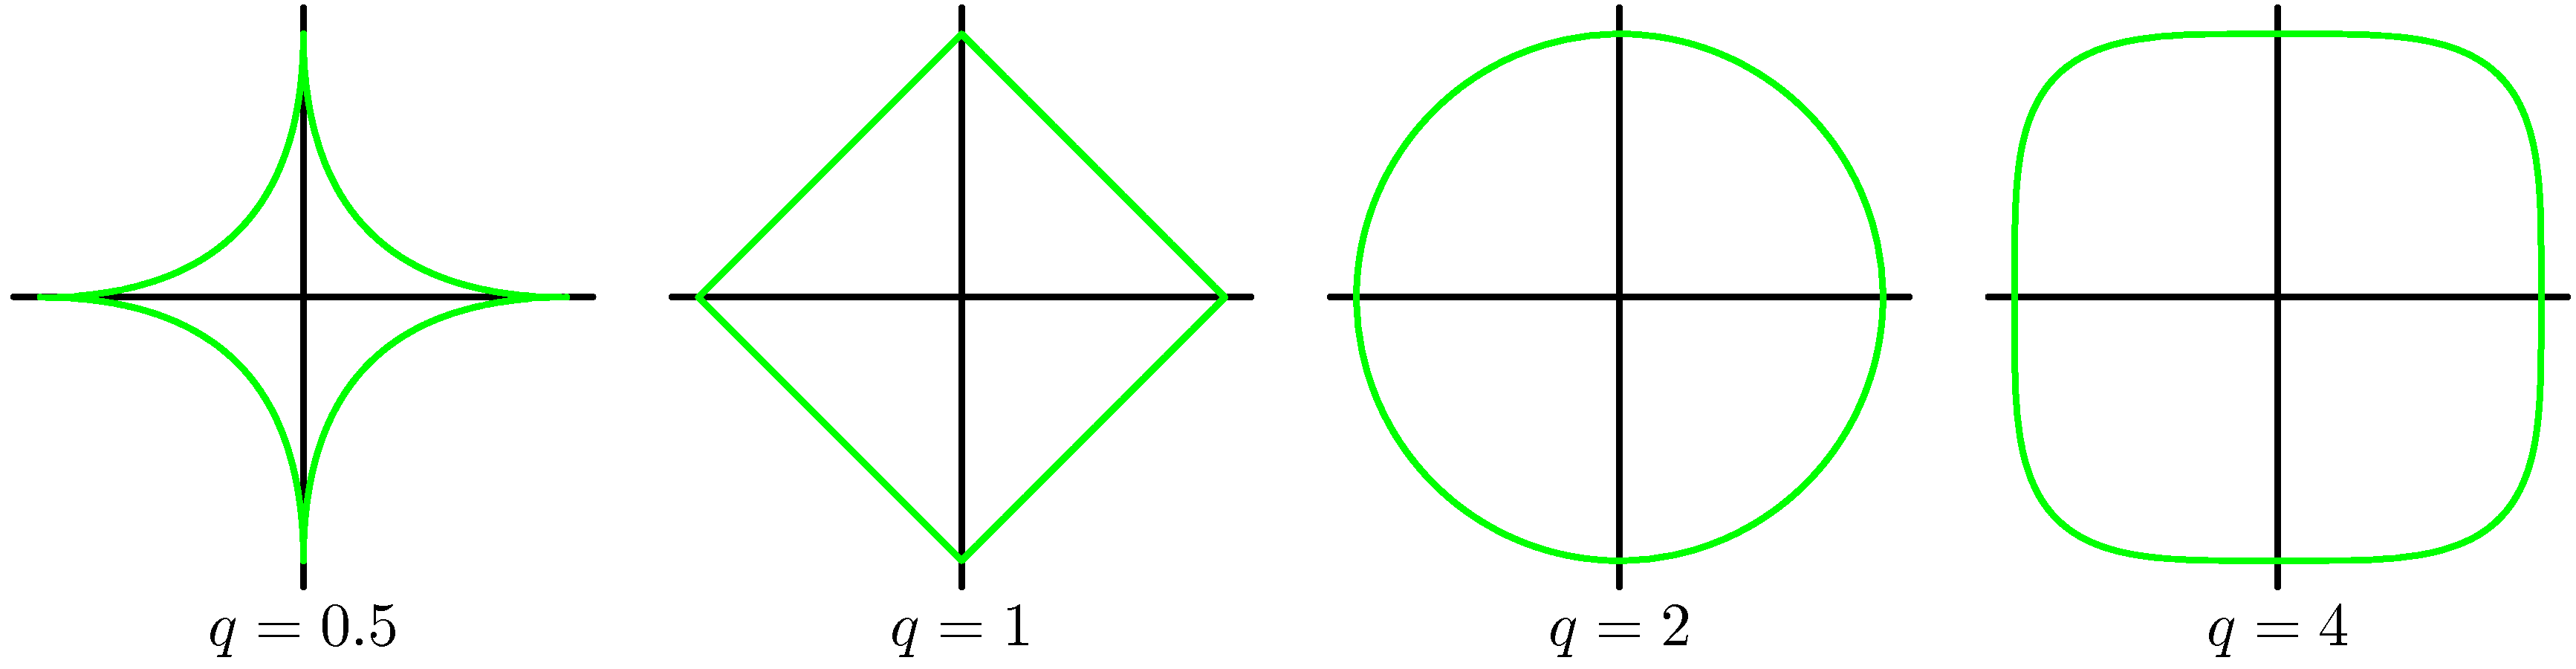
\includegraphics[scale=0.8]{Images/3-3.png}
		\captionsetup{font={small}}
		\caption{正则项(3.29)在$q$取不同值时的图像}
		\label{fig:3-3}
	\end{figure}
	\\
	\indent 如果$q=1$那么就变成了统计学中的lasso方法(Tibshirani, 1996)。如果$\lambda$充分大,那么某些系数$w_j$会变成0,会形成基底函数不起作用的稀疏模型(sparse model)。为了验证这一点,首先要留意到,对(3.29)进行最小化等价于将未正则化的平方和误差(3.12)在带有适当参数$\eta$的以下约束下进行最小化\textcolor{red}{\textbf{——习题 3.5}}
	\begin{equation}
		\sum_{j=1}^M |w_j|^q \leqslant \eta
	\end{equation}
	这样就可以利用拉格朗日乘数法将两种方法结合起来\textcolor{red}{\textbf{——附录 E}}。误差函数在约束条件(3.30)下的最小值,也就是稀疏性的来源如图3.4所示。随着$\lambda$的增加,变成0的参数数量也在不断增加。
	\begin{figure}[ht]
		\begin{minipage}[t]{0.5\linewidth}
		\centering
		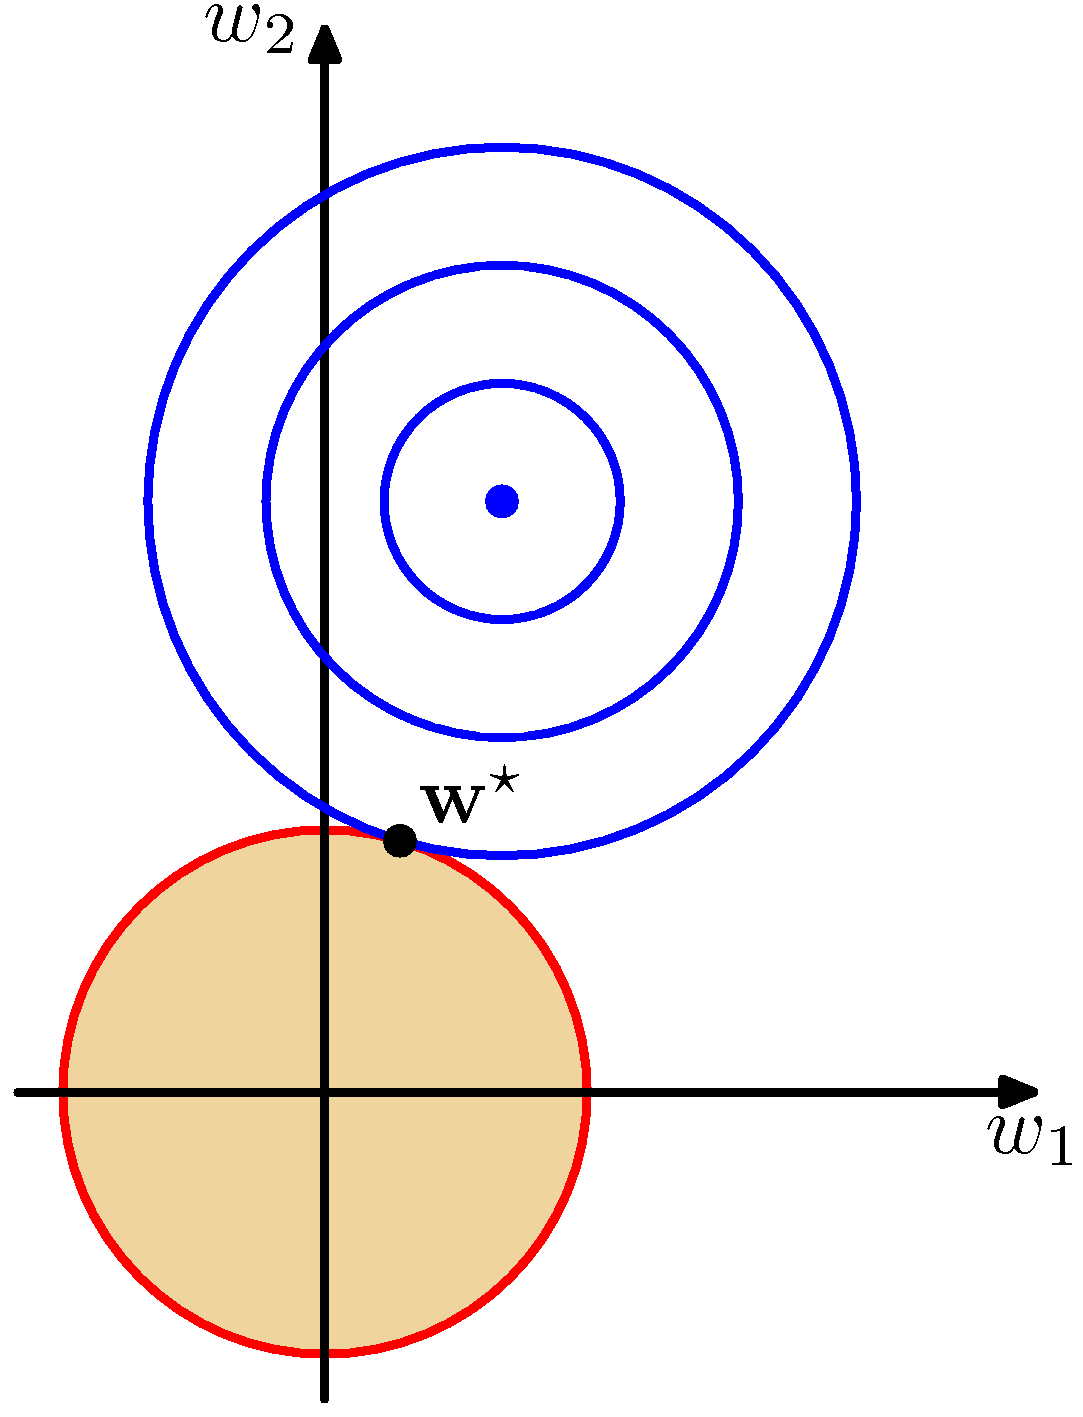
\includegraphics[scale=0.8]{Images/3-4a.png}
		\label{fig:3-4a}
		\end{minipage}
		\begin{minipage}[t]{0.5\linewidth}
		\centering
		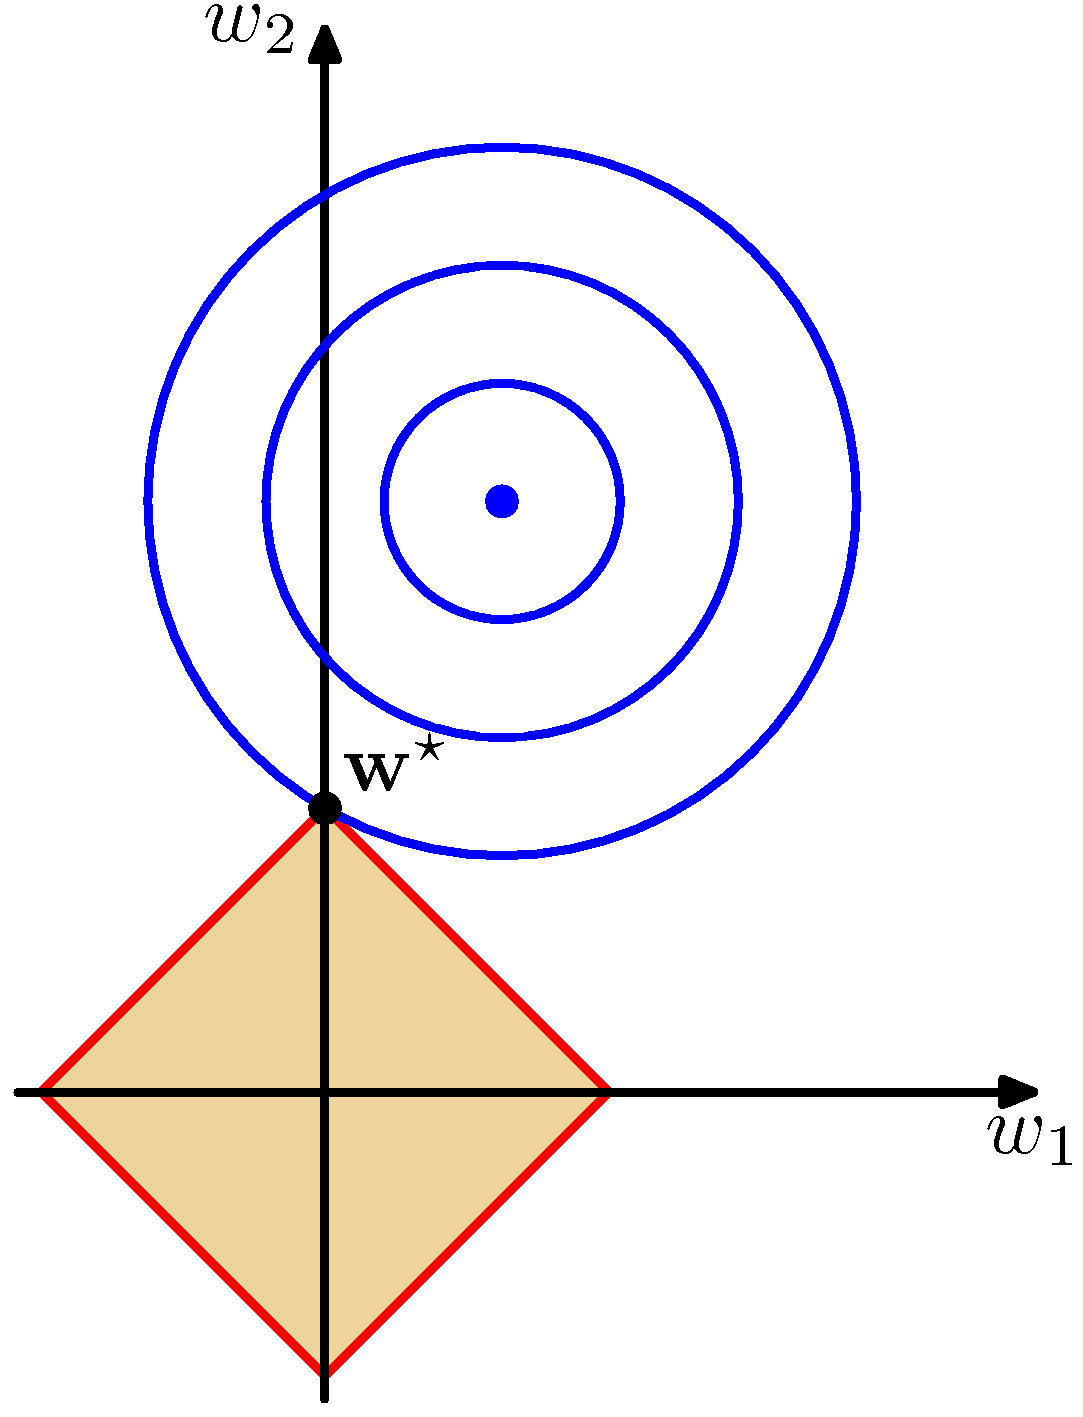
\includegraphics[scale=0.8]{Images/3-4b.png}
		\label{fig:3-4b}
		\end{minipage}
		\captionsetup{font={small}}
		\caption{未正则化的误差函数(蓝色曲线)与$q=2$(二次正则项,左)和1(lasso正则项,右)时的约束区域(3.30),参数向量$\bw$的最优解为$\bw^{\star}$。lasso正则项可以给出$w_1^{\star}=0$这样的稀疏解。}
	\end{figure}
	\\
	\indent 正则化可以通过限制有效模型的复杂度,在有限大小的数据集上训练出复杂的模型,同时避免严重过拟合的情况出现。然而,确定模型的最优复杂度这一问题就从寻找合适的基底函数数量变成了确定合适的正则化系数$\lambda$。我们将在本章后面的内容中回到这个问题。\\
	\indent 考虑到实际应用和分析计算的简便,在本章的剩余内容中我们主要使用二次正则项(3.27)。
	}
	\subsection{多项输出}
	\textnormal{
	到目前为止我们一直在研究单一目标变量$t$的情况。但在一些实际应用中,我们还可能会希望得到$K > 1$个目标变量,可以写成向量$\mathbf{t}$。这可以利用对$\mathbf{t}$的每个分量都使用不同的基底函数,于是问题就拆分成了所有分量相互无关的回归问题。然而更加常见的方法是对目标变量的分量采用相同的基底函数
	\begin{equation}
		\mathbf{y}(\bx, \bw) = \mathbf{W}^{\rmT} \bfphi(\bx) 
	\end{equation}
	其中的$\mathbf{y}$为$K$维列向量,$\mathbf{W}$为$M \times K$维的参数矩阵,$\bfphi(\bx)$为$M$维的列向量,其元素为$\phi_j(\bx)$,且$\phi_0(\bx)=1$。如果我们假设目标向量的条件分布是各向同性的高斯分布,
	\begin{equation}
		p(\mathbf{t}|\bx,\mathbf{W},\beta) = \calN (\mathbf{t}|\mathbf{W}^{\rmT}\bfphi(\bx),\beta^{-1}\mathbf{I})
	\end{equation}
	如果观测数据为$\mathbf{t}_1,...,\mathbf{t}_N$,那么就可以将它们集合在矩阵$\mathbf{T}$中,$\mathbf{T}$为$N \times K$维的矩阵,且它的第$n$行就是$\mathbf{t}_n^{\rmT}$。类似地,我们也可以把输入向量$\bx_1, ..., \bx_N$集合成矩阵$\mathbf{X}$。那么对数似然函数就可以写成
	\begin{equation}
	\begin{split}
		\ln p(\mathbf{T}|\mathbf{X,W},\beta) &= \sum_{n=1}^N \ln \calN(\mathbf{t}_n|\mathbf{W}^{\rmT}\bfphi(\bx_n),\beta^{-1}\mathbf{I})\\
		&= \frac{NK}{2}\ln \left(\frac{\beta}{2\pi}\right) -\frac{\beta}{2}\sum_{n=1}^N \|\mathbf{t}_n - \mathbf{W}^{\rmT} \bfphi(\bx_n)\|^2
	\end{split}
	\end{equation}
	和以前一样,可以对似然函数关于$\mathbf{W}$进行最大化,得到的解为
	\begin{equation}
		\mathbf{W}_{\mathrm{ML}} = (\bfPhi^{\rmT} \bfPhi)^{-1} \bfPhi^{\rmT} \mathbf{T}
	\end{equation}
	如果对每个目标变量$t_k$都做一下验证,那么
	\begin{equation}
		\bw_k = (\bfPhi^{\rmT} \bfPhi)^{-1} \bfPhi^{\rmT} \sft_k = \bfPhi^{\dagger}\sft_k
	\end{equation}
	其中$\sft_k$为$t_{nk}, n=1,...,N$组成的$N$维列向量。于是回归问题的解就拆分开了,而且只需要计算一个伪逆矩阵$\bfPhi^{\dagger}$,因为这个矩阵是所有向量$\bw_k$所共用的。\\
	\indent 这些结论可以直接推广到带有一般的协方差矩阵的高斯噪声分布中。\textcolor{red}{\textbf{——习题 3.6}}\ 和上述情况一样,这样可以将回归问题拆分成$K$个相互独立的回归问题。这样的结果并不很出人意料,因为参数$\mathbf{W}$仅与高斯噪声分布的均值有关,而且从第2.3.4节中我们可以得知,多元高斯分布均值的最大似然解是与协方差无关的。所以从现在开始,为了简化起见,我们会一直对单一目标变量$t$进行讨论。
	}
	\section{偏差-方差分解}
	\insertline\\
	\textnormal{
	\indent 到目前为止所讨论的线性回归模型中,我们都做了这样的假设,即基底函数的形式和数量都是确定的。根据第1章中的相关内容,使用最大似然法(或者最小二乘法)可能会导致过拟合,尤其是在较小的数据集上训练复杂模型的时候更容易出这个问题。然而,为了防止过拟合的出现而限制基底函数的数量的话也会造成负面的影响,因为这样的做法严重限制了模型的灵活性,使得模型抓住数据中关键规律的能力下降。尽管加入正则项可以控制参数较多的模型出现过拟合的可能,但如何确定正则项系数$\lambda$又成了一个新的问题。通过将正则化误差函数关于权重向量$\bw$和正则化系数$\lambda$求取最小化来求正则项系数的做法明显不可靠,因为很明显最后的结果一定是$\lambda = 0$。\\
	\indent 在从前的讨论中我们可以看出,容易造成过拟合现象是最大似然方法的极大劣势,不过在贝叶斯方法的参数边缘化时完全不会出现这个问题。在本章中我们将使用贝叶斯观点研究模型的复杂度。不过在此之前,先来研究一个频率域观点的模型复杂度问题,即偏差-方差(bias-variance)之间的权衡。尽管我们将在线性基底函数模型的背景下介绍这个概念,毕竟解释起来比较简单,但这个内容并非局限于此,对于其他的模型也是适用的。\\
	\indent 在第1.5.5节中研究回归问题的决策论时,我们探究了一些损失函数,在给定条件分布$p(t|\bx)$时,每种损失函数都可以得到相应的最优预测。比较广泛的选择是平方损失函数,其对应的最优预测为条件期望,将其表示为$h(\bx)$,那么
	\begin{equation}
		h(\bx) = \mathbb{E}[t|\bx] = \int t p(t|\bx)\ \mathrm{d}t
	\end{equation}
	此时需要区分一下决策论中的平方损失函数与模型参数最大似然估计中的平方和误差函数。这里可能会用到类似正则化或完整贝叶斯方法这样比最小二乘法更加复杂的方法来确定条件分布$p(t|\bx)$。在进行预测时,它们都可以与平方损失函数相结合。\\
	\indent 在第1.5.5节中已经证明了期望平方损失可以写成如下形式:
	\begin{equation}
		\mathbb{E}[L]=\int \{y(\bx) - h(\bx)\}^2 p(\bx)\ \mathrm{d}\bx + \iint \{h(\bx)-t\}^2 p(\bx, t)\ \mathrm{d}\bx \ \mathrm{d}t
	\end{equation}
	回想一下,与$y(\bx)$无关的第2项是由于数据中的噪声而出现的,表示的是期望误差所能达到的最小的值。第1项与函数$y(\bx)$的选择有关,所以我们要做的就是选择一个使得该项取得最小值的$y(\bx)$。由于这是一个非负项,所以它所能达到的最小值是0。如果数据是无限的(而且计算资源也是无限的),原则上来说我们可以得到任意精确度的回归函数$h(\bx)$,也就随之得到了最佳的$y(\bx)$。然而实际应用中可不会这么理想,数据集$\mathcal{D}$是有限的,于是回归函数$h(\bx)$的精确形式也就无从知晓了。\\
	\indent 如果使用带有参数$\bw$的函数$y(\bx,\bw)$对$h(\bx)$进行建模,那么根据贝叶斯观点,模型的不确定性就可以通过$\bw$的后验分布来表示。然而频率域的方法却是要基于数据集$\mathcal{D}$对参数$\bw$进行点估计,并根据如下思路来解释估计的不确定性。假设有很多个大小为$N$的数据集,每个数据集都是相互独立地从分布$p(t,\bx))$中获取的。对于任意的数据集$\mathcal{D}$都可以进行学习并得到相应的预测函数$y(\bx;\mathcal{D})$。这堆不同的数据集会各自给出不同的预测函数,所以相应也会得到不同的平方损失,然后根据这些数据集上的平均值确定学习算法的性能。\\
	\indent 对于(3.37)中的第1项,假设数据集已经钦定为$\mathcal{D}$,那么积分项中的第1项就变成了
	\begin{equation}
		\{y(\bx;\mathcal{D})-h(\bx)\}^2
	\end{equation}
	由于这一项的值与数据集$\mathcal{D}$的选择有关,所以要在不同的数据集上取平均值。在大括号中加上一个$\mathbb{E}_{\mathcal{D}}[y(\bx;\mathcal{D})]$再马上减掉,并做点处理,可以得到
	\begin{equation}
	\begin{split}
		&\{y(\bx;\mathcal{D})-\mathbb{E}_\mathcal{D}[y(\bx;\mathcal{D})] + \mathbb{E}_\mathcal{D}[y(\bx;\mathcal{D})] -h(\bx)\}^2 \\
		= &\{y(\bx;\mathcal{D})-\mathbb{E}_\mathcal{D}[y(\bx;\mathcal{D})]\}^2 + \{\mathbb{E}_\mathcal{D}[y(\bx;\mathcal{D})] - h(\bx)\} \\
		&+ 2\{y(\bx;\mathcal{D})-\mathbb{E}_\mathcal{D}[y(\bx;\mathcal{D})]\}\{\mathbb{E}_\mathcal{D}[y(\bx;\mathcal{D})]-h(\bx)\}
	\end{split}
	\end{equation}
	关于$\mathcal{D}$求期望,此时第1项就会消失了,于是
	\begin{equation}
	\begin{split}
		&\mathbb{E}_{\mathcal{D}}[\{y(\bx;\mathcal{D})-h(\bx)\}^2] 	= \underbrace{\{\mathbb{E}_\mathcal{D}[y(\bx;\mathcal{D})]-h(\bx)\}^2}_{\textcolor{blue}{(\mathrm{bias})^2}} + \underbrace{\mathbb{E}_{\mathcal{D}}[\{y(\bx;\mathcal{D})-\mathbb{E}_\mathcal{D}[y(\bx;\mathcal{D})]\}^2]}_{\textcolor{red}{\mathrm{variance}}}
		\end{split}
	\end{equation}
	可以看出$y(\bx;\mathcal{D})$与回归函数$h(\bx)$之间的期望平方差可以拆分成两项的和。第1项是偏差(bias)的平方,表示所有数据集的预测结果的平均值与回归函数之间的差异。第2项是方差(variance),表示对于每一个数据集,模型给出的解在其平均值附近变化的程度,也就是函数$y(\bx)$对于数据集选择的敏感程度。我们会通过一个简单的案例来解释这些概念。\\
	\indent 到目前为止,我们研究的都是单一的输入$\bx$。如果将这个展开形式代入(3.37)中,可以得到期望平方损失的拆分形式:
	\begin{equation}
		\mathrm{expected\ loss = (bias)^2 + variance + noise}
	\end{equation}
	其中
	\begin{align}
		\mathrm{(bias)^2} &= \int \{\mathbb{E}_{\mathcal{D}}[y(\bx;\mathcal{D})]-h(\bx)\}^2 p(\bx)\ \mathrm{d}\bx\\
		\mathrm{variance} &= \int \mathbb{E}_{\mathcal{D}}[\{y(\bx;\mathcal{D}) - \mathbb{E}_{\mathcal{D}}[y(\bx;\mathcal{D})]\}^2]p(\bx)\ \mathrm{d}\bx \\
		\mathrm{noise} &= \int \{h(\bx)-t\}^2 p(\bx,t)\ \rmd \bx \ \rmd t
	\end{align}
	现在偏差项和方差项的定义变成了积分后的值。\\
	\indent 我们的目标是将期望损失最小化,而且已经把它拆分成了偏差的平方、方差和噪声常数项的和。我们即将会进行偏差与方差之间的制衡,低偏差高方差的模型会具有很高的灵活性,而高偏差低方差的模型会具有很高的稳定性。将偏差与方差完美均衡的模型就是具有最好预测性能的模型。这里还是用第1章中的正弦函数数据集说事。\textcolor{red}{\textbf{——附录 A}}\ 假设现在生成成了100个数据集,每个数据集包含$N=25$个数据,所有数据都是各自独立地从正弦曲线$h(x) = \sin (2 \pi x)$中获取的。数据集的编号为$l = 1, ..., L, L=100$,且对于所有的数据集$\mathcal{D}^{(l)}$,都使用包含24个高斯基底函数的模型进行拟合,拟合的过程是通过将正则误差函数(3.27)进行最小化来完成的,从而给出预测函数$y^{(l)}(x)$,如图3.5所示。其中,第1行的结果是通过一个较大的正则化系数$\lambda$得到的,这样的模型方差很小(第1行左图中各个曲线相差不大),但偏差很大(第1行右图中与真实曲线相比差别非常大)。与之不同的是,第3行的结果是通过一个较小的正则化系数$\lambda$得到的,这样的模型方差很大(第3行左图中各个曲线相差很大),但偏差很小(取平均值之后就与真实曲线很接近了)。需要注意的是,将这个复杂模型的$M=25$个解求平均值,可以对回归函数产生很好的拟合结果,说明求平均值是一个很不错的想法。实际上,对多个解求取加权平均值是贝叶斯方法的核心,不过这里的求平均值针对的是参数的后验分布而非数据集。\\
	\indent 我们可以顺便利用这个例子研究一下偏差-方差的制衡。预测的平均值为
	\begin{equation}
		\overline{y}(x) = \frac{1}{L} \sum_{l=1}^L y^{(l)}(x)
	\end{equation}
	\newpage
	\begin{figure}[H]
		\begin{minipage}[t]{0.5\linewidth}
		\centering
		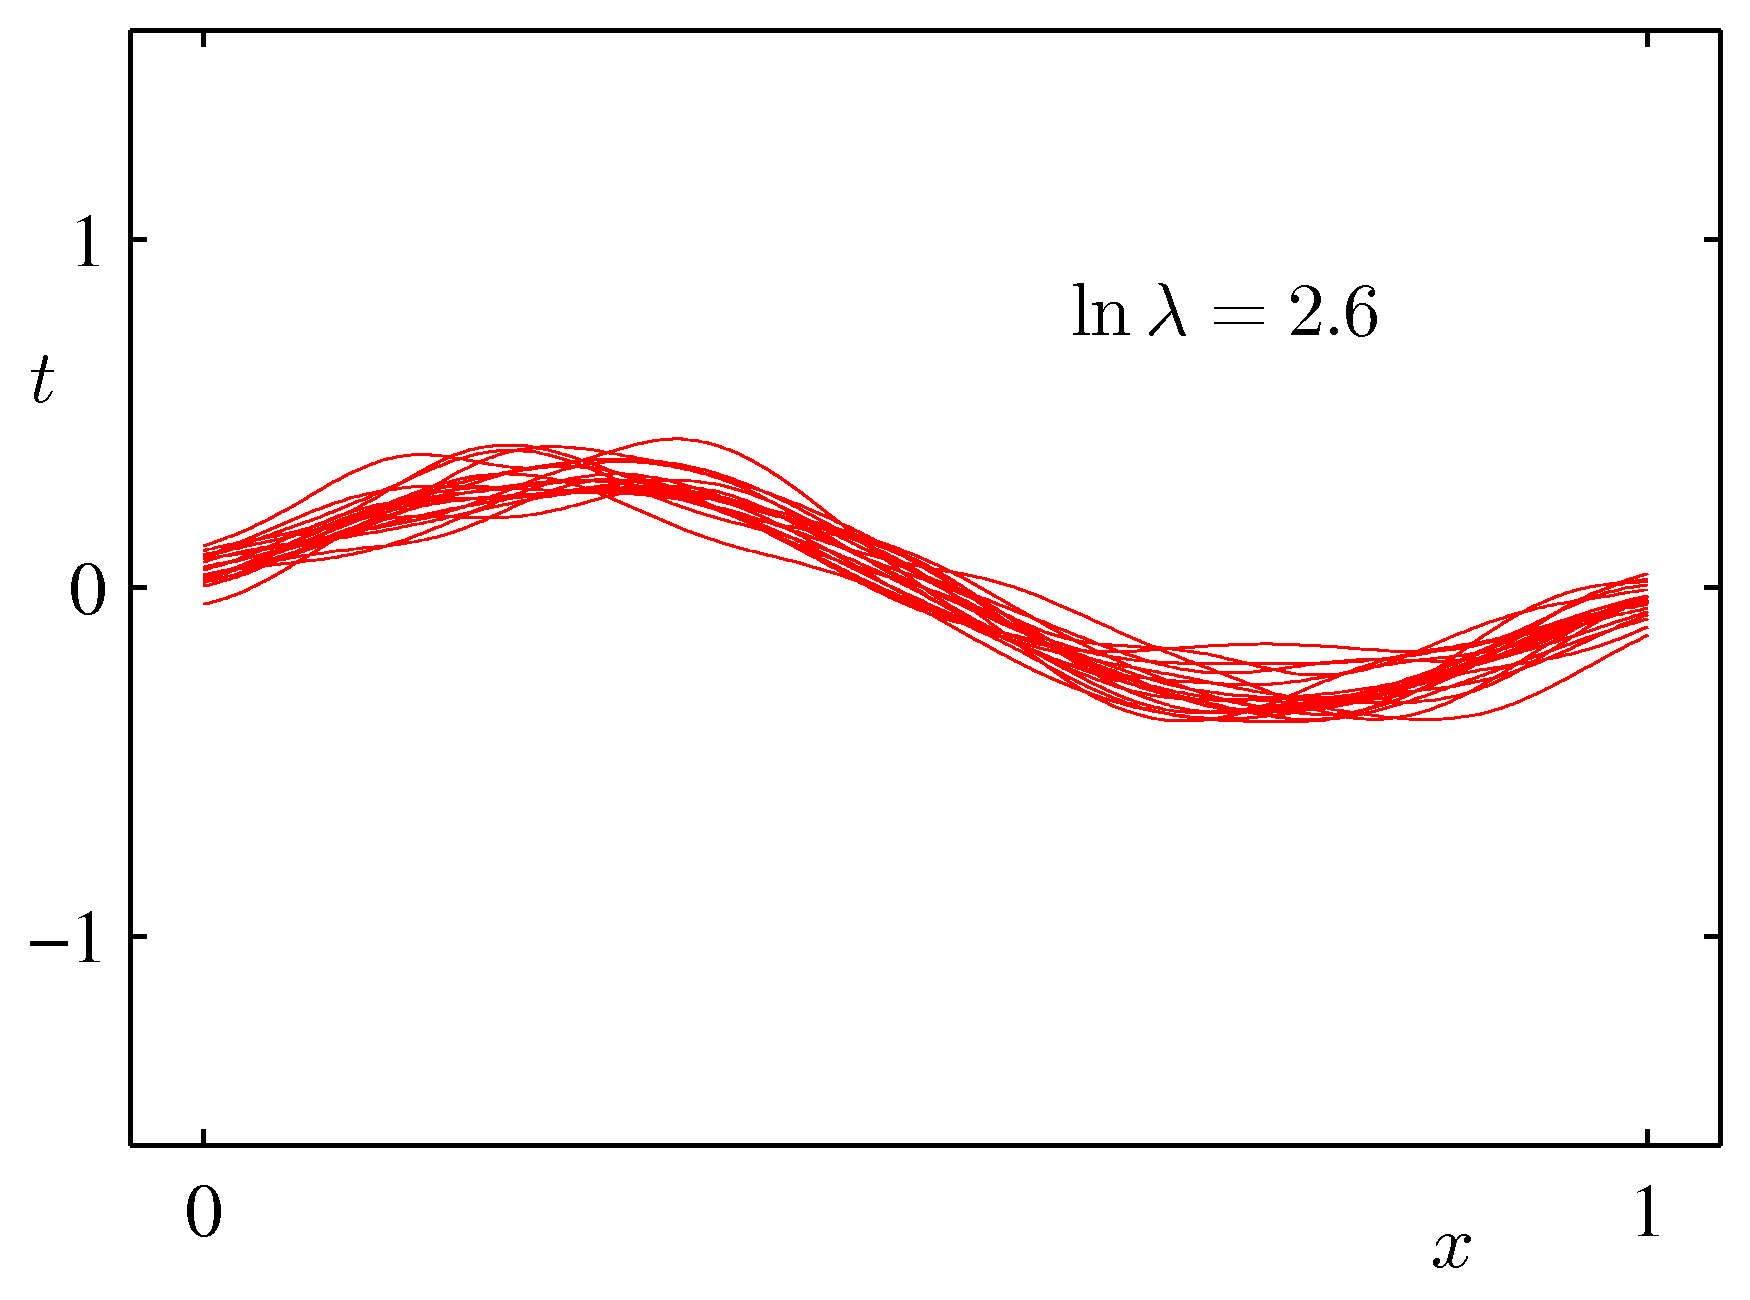
\includegraphics[scale=0.8]{Images/3-5a.png}
		\label{fig:3-5a}
		\end{minipage}
		\begin{minipage}[t]{0.5\linewidth}
		\centering
		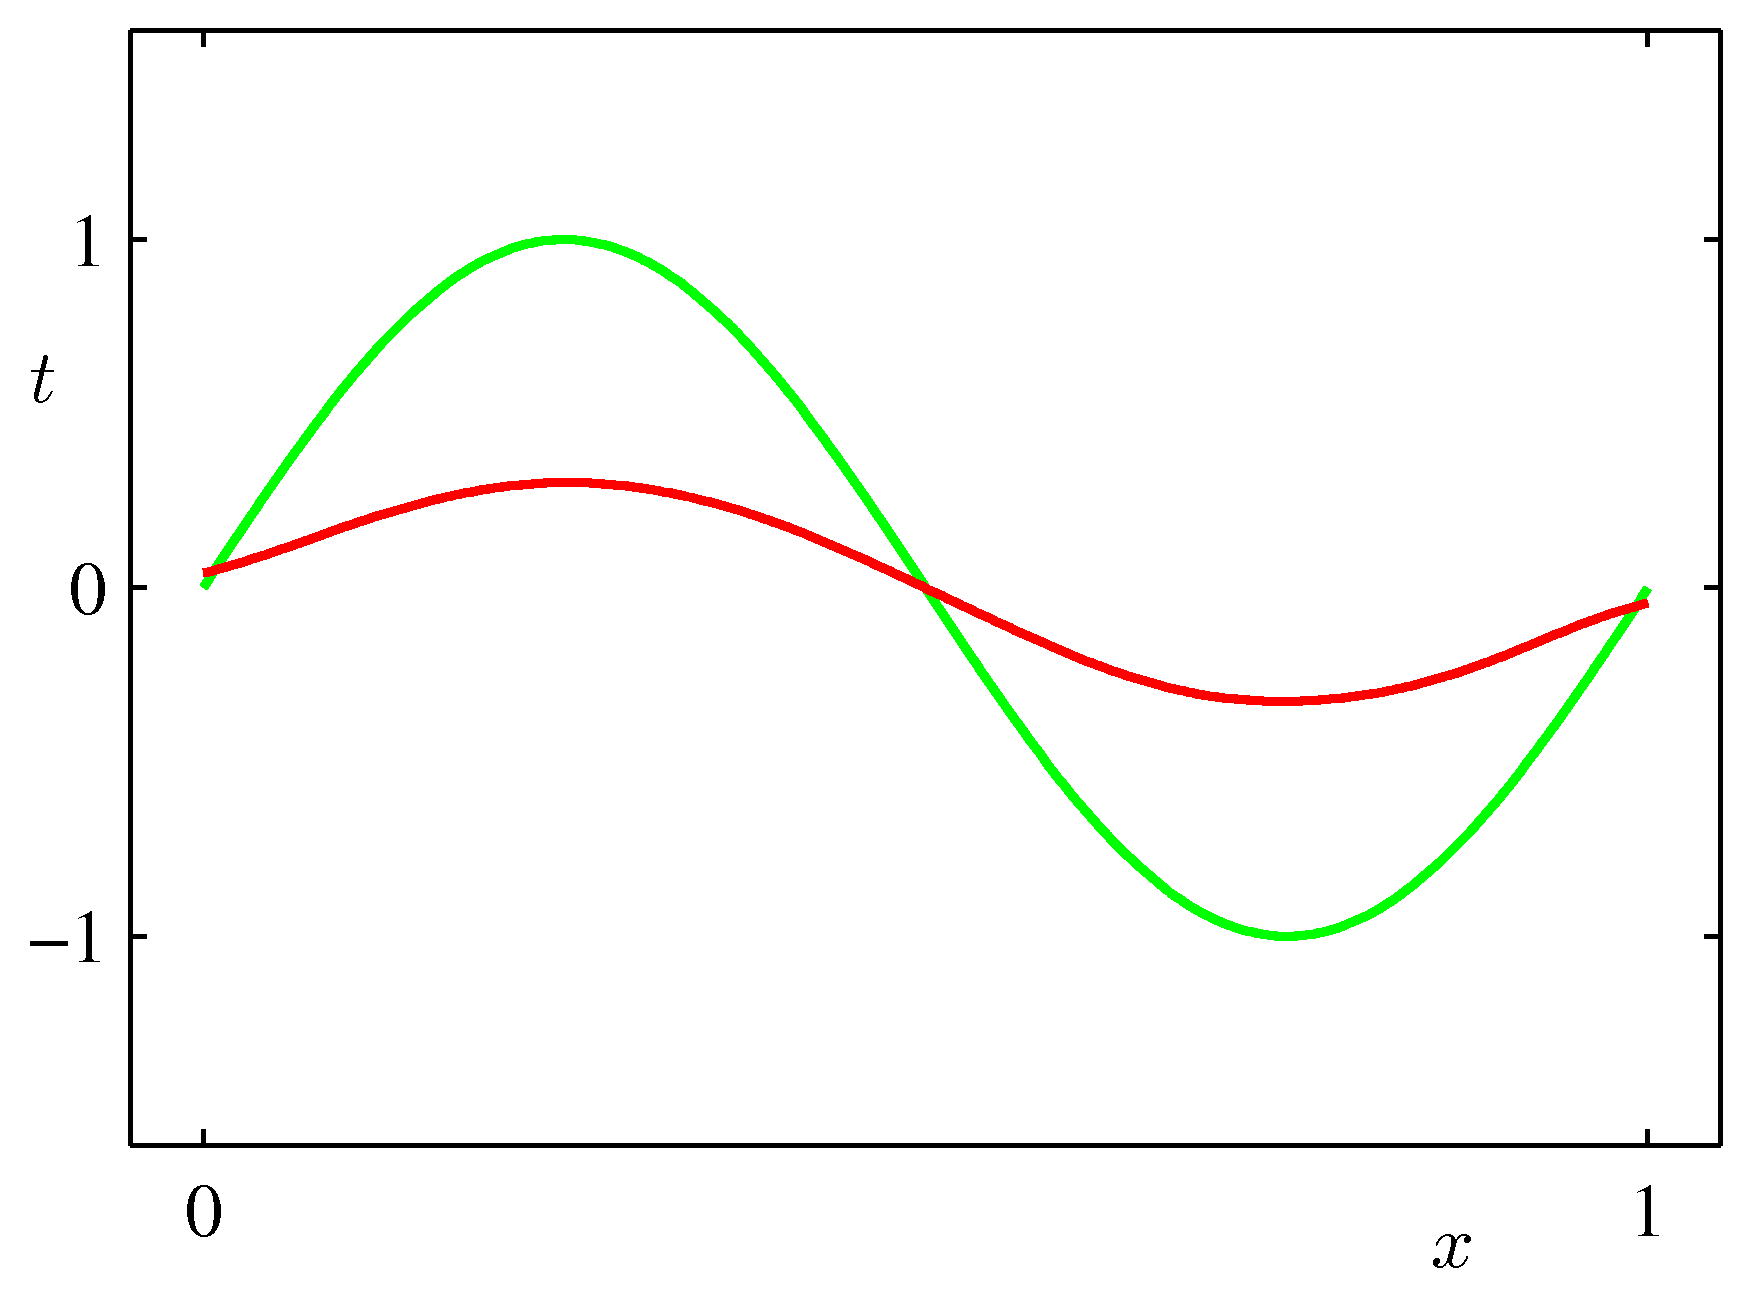
\includegraphics[scale=0.8]{Images/3-5b.png}
		\label{fig:3-5b}
		\end{minipage}\\
		\begin{minipage}[t]{0.5\linewidth}
		\centering
		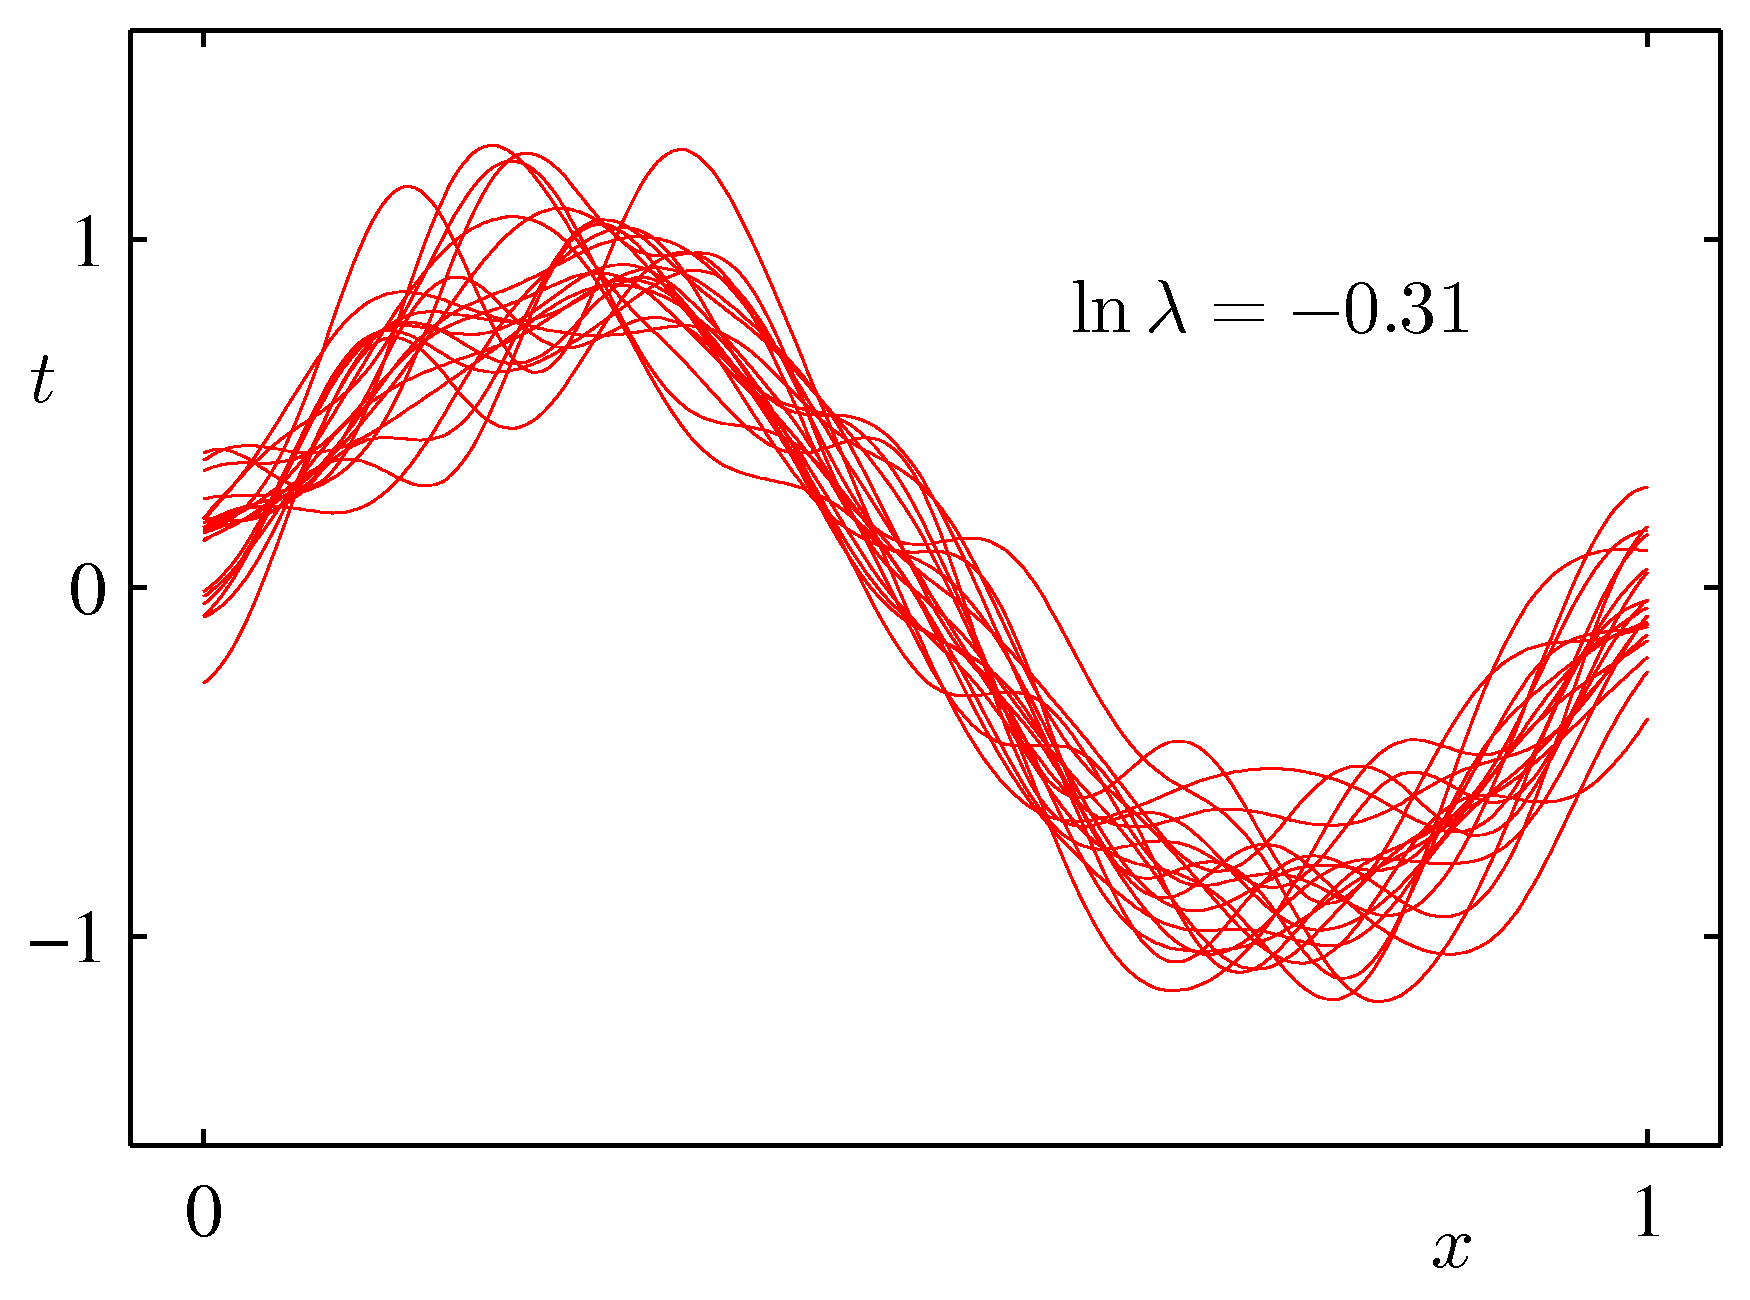
\includegraphics[scale=0.8]{Images/3-5c.png}
		\label{fig:3-5c}
		\end{minipage}
		\begin{minipage}[t]{0.5\linewidth}
		\centering
		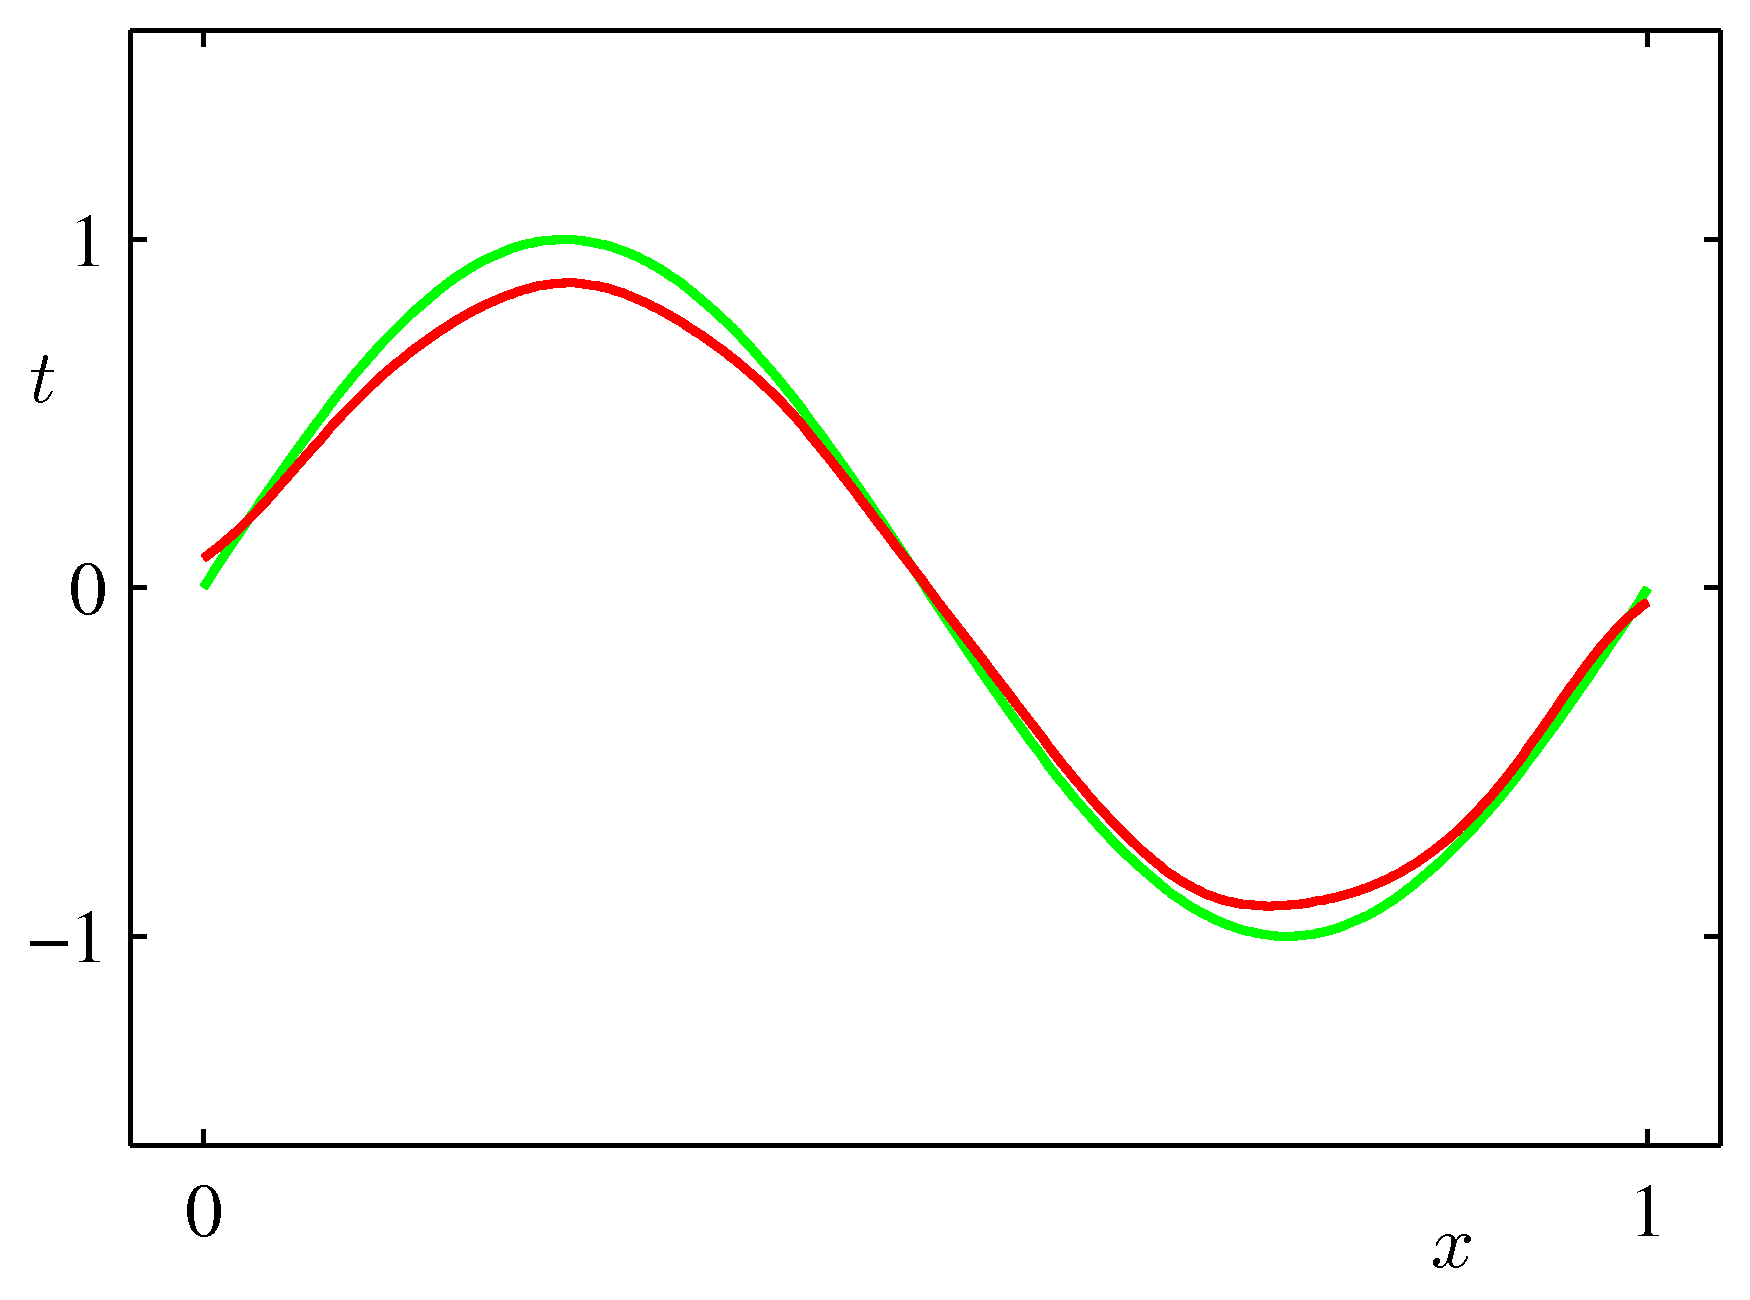
\includegraphics[scale=0.8]{Images/3-5d.png}
		\label{fig:3-5d}
		\end{minipage}\\
		\begin{minipage}[t]{0.5\linewidth}
		\centering
		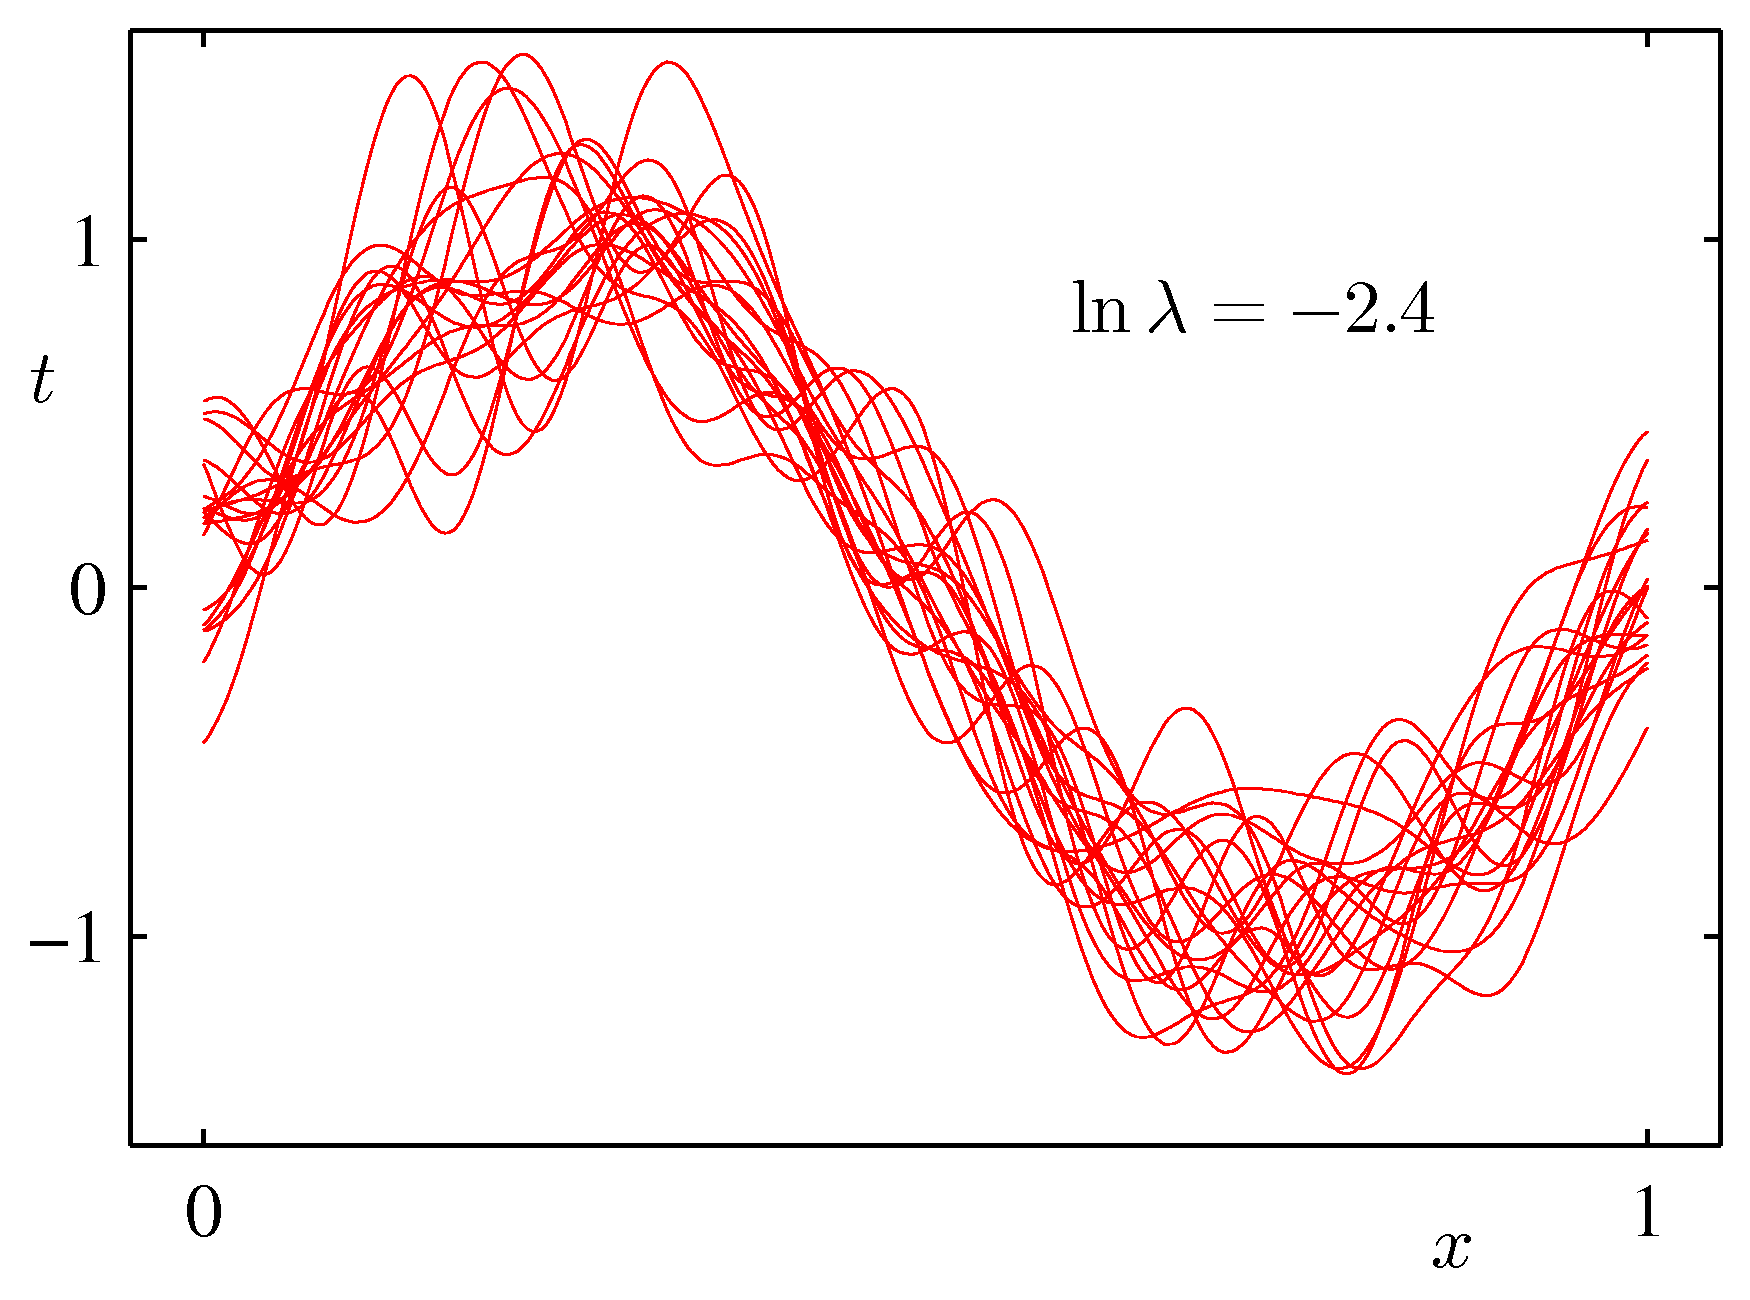
\includegraphics[scale=0.8]{Images/3-5e.png}
		\label{fig:3-5e}
		\end{minipage}
		\begin{minipage}[t]{0.5\linewidth}
		\centering
		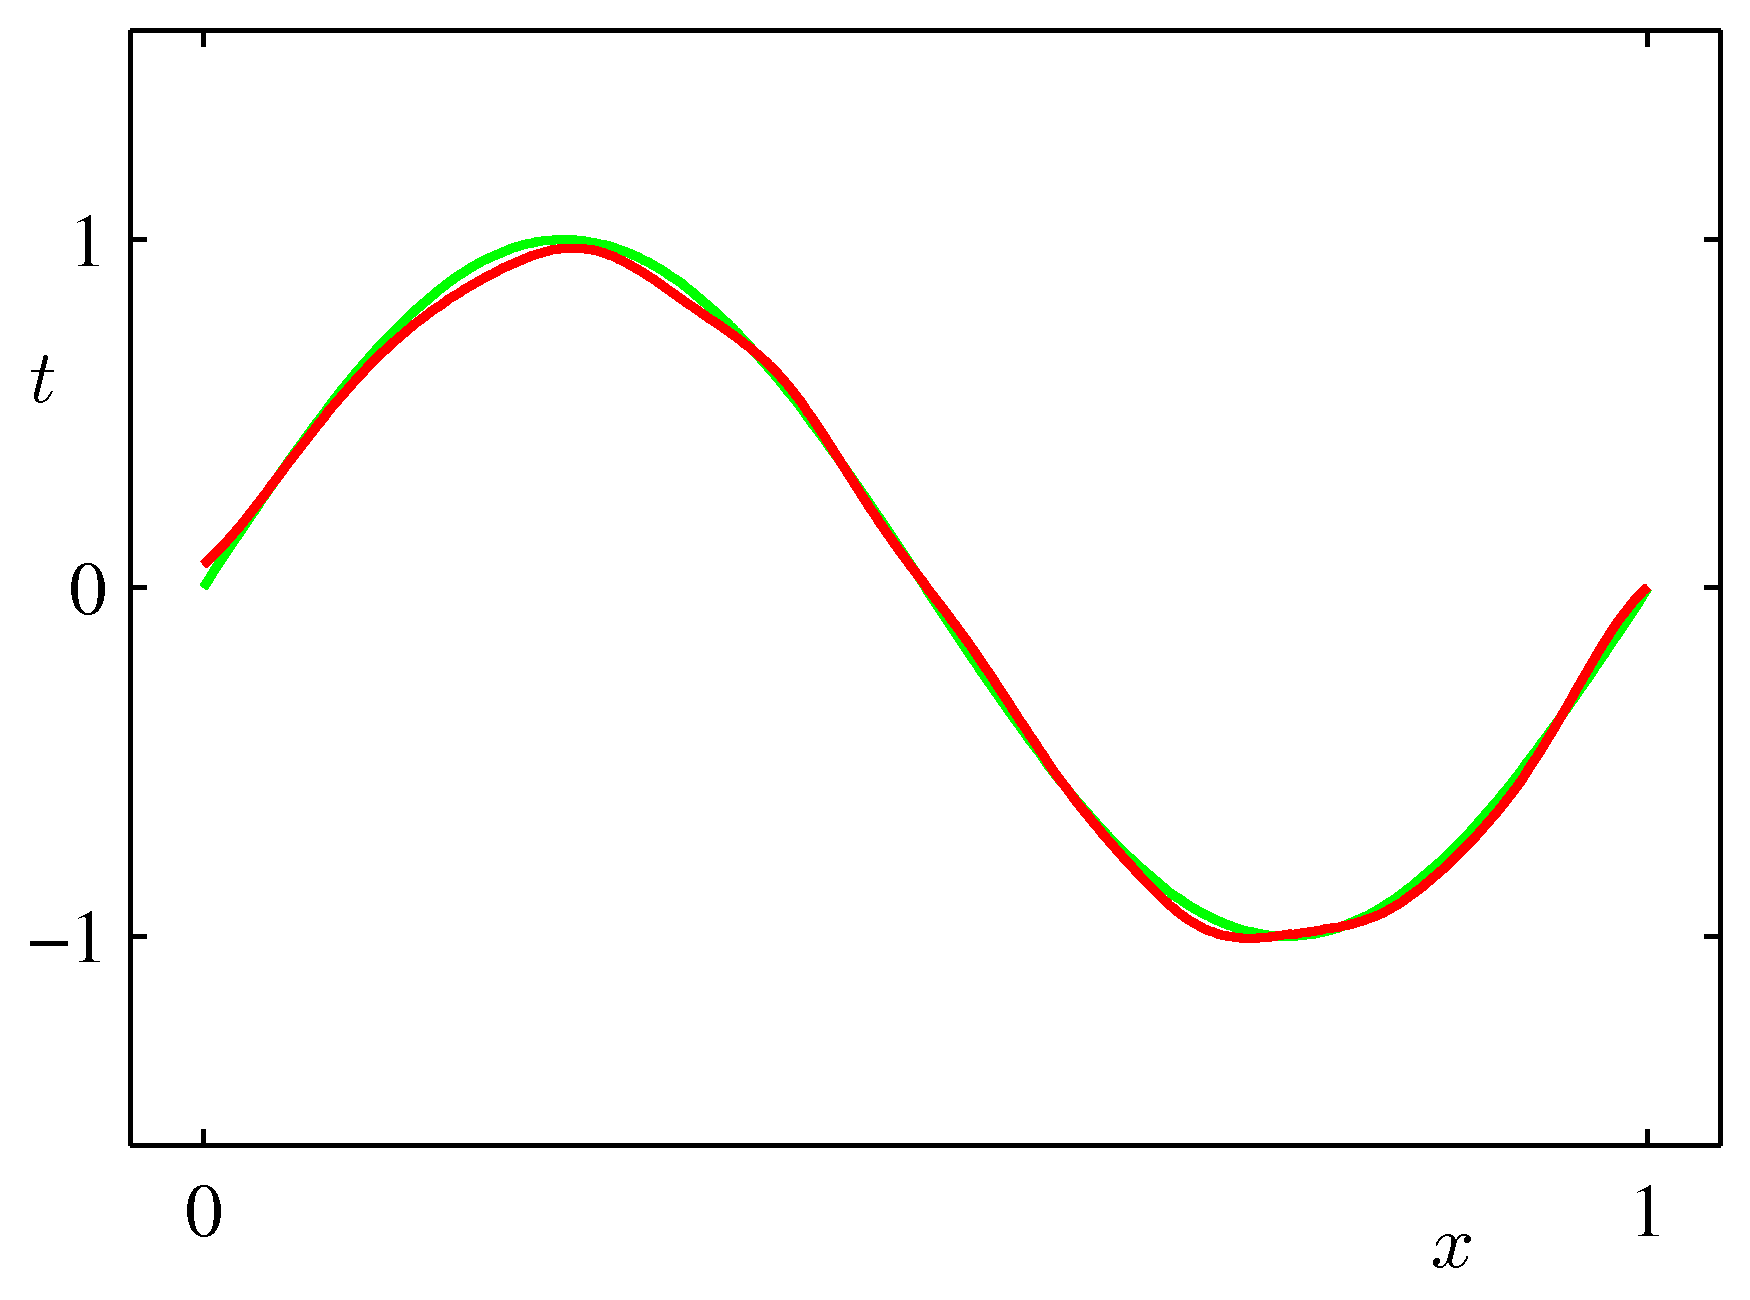
\includegraphics[scale=0.8]{Images/3-5f.png}
		\label{fig:3-5f}
		\end{minipage}
		\captionsetup{font={small}}
		\caption{偏差和方差与模型复杂度相关,模型的复杂度由参数$\lambda$控制,利用第1章中的正弦函数数据集得到的结果。数据集的数量$L=100$,每个数据集里包含$N=25$组数据,模型中包含24个高斯基底函数,算上偏差参数,参数的总数为$M=25$。左侧一列展示的是在不同$\ln \lambda$下的模型拟合结果(为了简洁起见并没有把100个拟合结果全画出来,而是只画了20个)。右侧一列展示的是相应产生的平均拟合结果(红色曲线)和真实的正弦函数曲线(绿色曲线)。}
	\end{figure}
	经过积分的平方偏差和方差为
	\begin{align}
		\mathrm{(bias)}^2 &= \frac{1}{N} \sum_{n=1}^N \{\overline{y}(x_n) - h(x_n)\}^2 \\
		\mathrm{variance} &= \frac{1}{N} \sum_{n=1}^N \frac{1}{L} \sum_{l=1}^L \left\{y^{(l)}(x_n) - \overline{y}(x_n)\right\}^2
	\end{align}
	其中关于$x$的积分都带有权重$p(x)$,这个积分是通过对分布中取出的数据点集合进行求和来近似得到的。这些值和它们的和关于$\ln \lambda$的函数图像如图3.6所示。可以看出,较小的$\lambda$会让模型对不同数据集中的噪声产生拟合,导致了较大的方差。与之相反,如果$\lambda$的值比较大,就会把权重参数向0拉近,形成较大的偏差。
	\begin{figure}[ht]
		\centering
		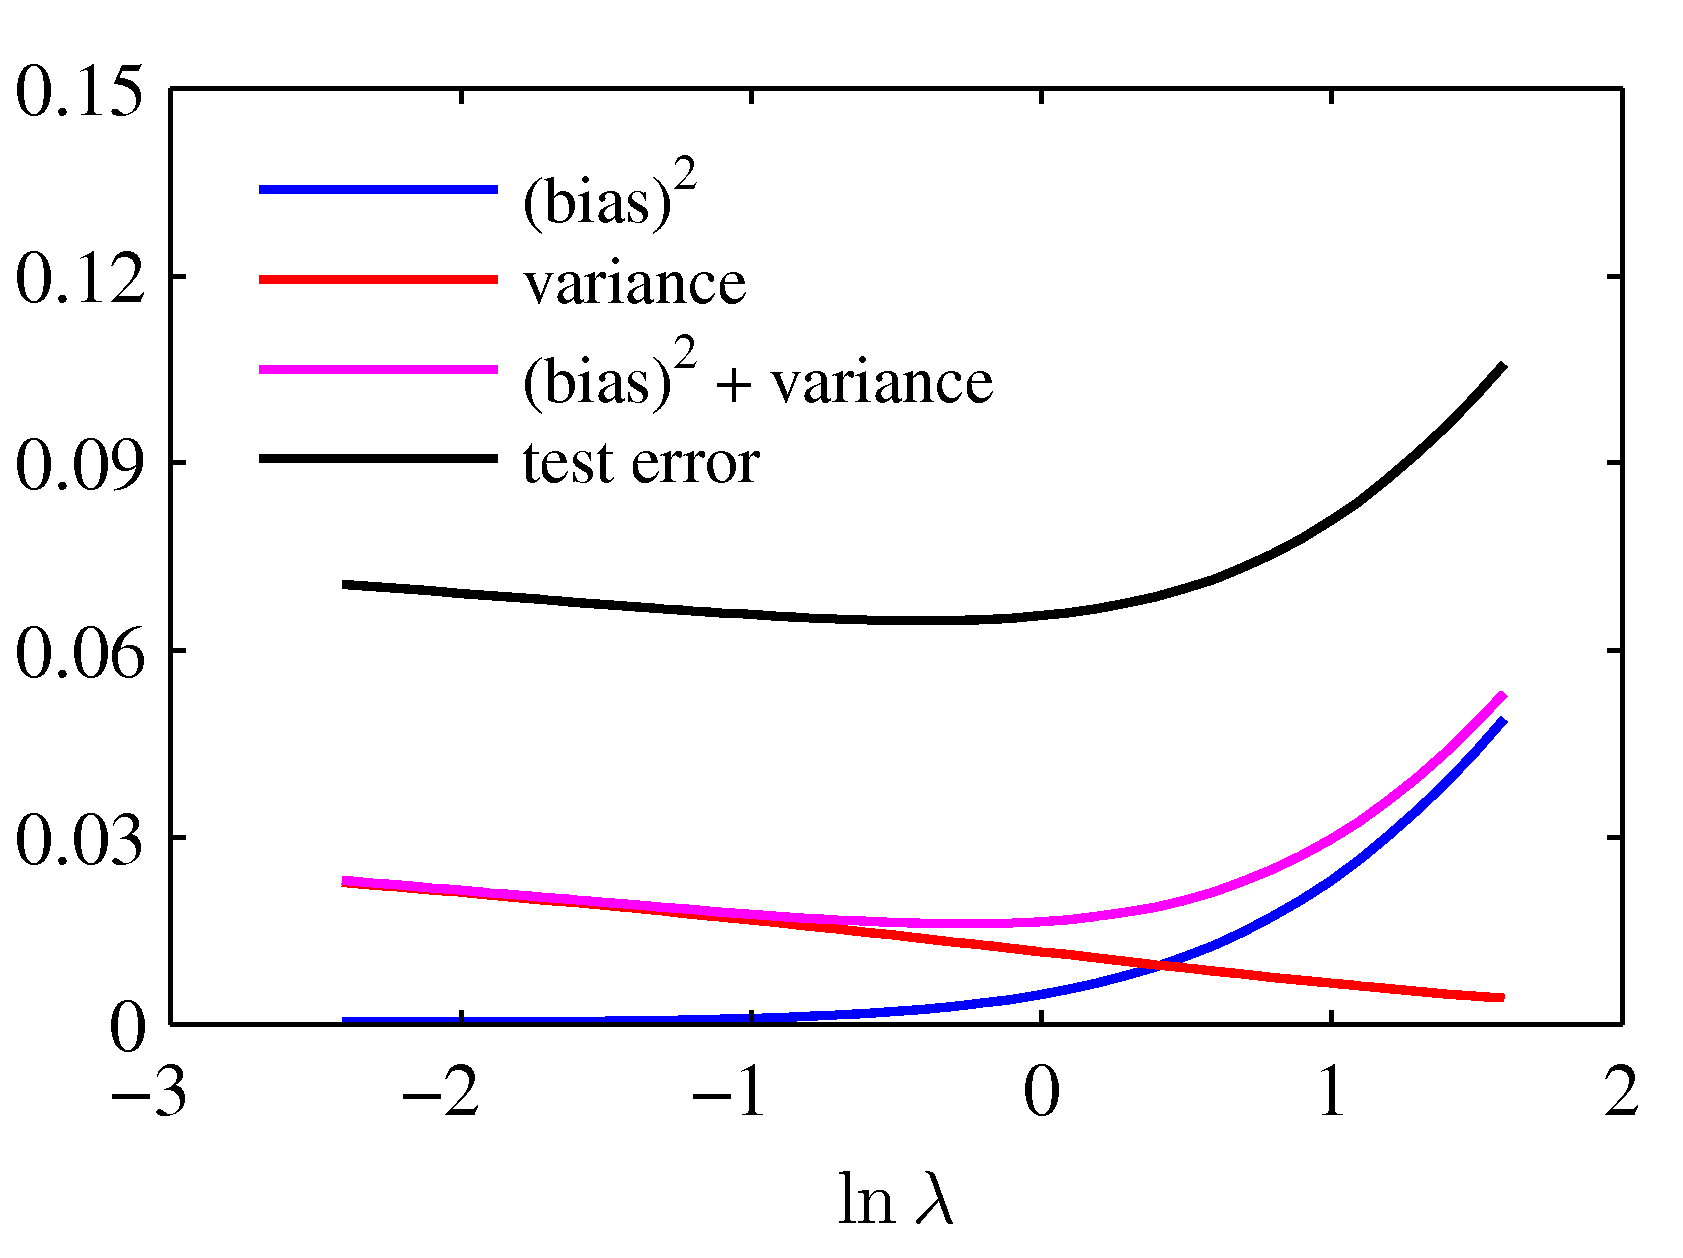
\includegraphics[scale=0.8]{Images/3-6.png}
		\captionsetup{font={small}}
		\caption{平方偏差、方差及其总和的图像,这个结果是对应图3.5的。同时也展示了一个包含1000个数据的测试集的平均误差。平方偏差+方差会在$\ln \lambda = -0.31$附近取得最小值,非常接近测试数据集上取得最小误差的位置。}
		\label{fig:3-6}
	\end{figure}
	\\
	\indent 尽管偏差-方差分解挺有意思,但实际应用中它的局限性相当明显,因为偏差-方差分解是要基于很多数据集求平均值的,然而在实际应用中,数据集可不一定有那么够用。如果训练集的数量非常大,我们也宁愿将它们全部汇总到一起,形成一个超大的数据集,因为这样做可以减少过拟合的出现。\\
	\indent 在知晓这种方法的局限性后,我们接下来进行贝叶斯视角的线性基底函数模型分析,这种方法对过拟合问题进行了更加深刻的分析,并给出了解决模型复杂度问题的实用方法。
	}
	\section{贝叶斯线性回归}
	\insertline \\
	\textnormal{
	\indent 我们从线性回归模型参数的最大似然方法中已经看出,模型的有效复杂度由基底函数的数量决定,而模型复杂度的选择应该取决于数据集的规模。在对数似然函数中加上一个正则项会影响到模型的有效复杂度,这样的做法使得模型复杂度可以由正则化系数来控制,不过基底函数的形式与数量仍然会对模型的性能产生重要的影响。\\
	\indent 那么这就遗留了一个问题,如何对实际的问题确定适当的模型复杂度,而且不能简单地通过对似然函数进行最大化得到,因为这样的做法往往会得到一个复杂的模型,而且容易出现过拟合的问题。在第1.3节中我们提到过,利用单独预分出来的数据可以确定模型的复杂度,但这样的做法很浪费计算资源也很浪费训练数据。于是我们转向了另一个思路,即利用贝叶斯观点处理线性回归问题,从而避免最大似然方法中可能出现的过拟合问题,而且可以仅通过训练数据就自动地确定模型的复杂度。为了方便起见,我们仍然针对一元目标变量$t$进行讨论。至于多元变量的情况,其实是可以由一元变量直接推广而来,可以参考一下第3.1.5节中的内容。
	}
	\subsection{参数分布}
	\textnormal{
	我们从模型参数$\bw$的先验概率分布入手,开始讨论贝叶斯方法的线性回归。现在开始,姑且认为噪声精度参数$\beta$是一个已知的常数。首先需要注意到,(3.10)中的似然函数$p(\sft | \bw)$是$\bw$的二次函数的指数。对应的共轭先验为如下的高斯分布,其均值为$\mathbf{m}_0$,协方差为$\mathbf{S}_0$:
	\begin{equation}
		p(\bw) = \calN (\bw|\mathbf{m}_0, \mathbf{S}_0)
	\end{equation}
	\indent 接下来计算后验分布,后验分布很明显是与先验和似然函数的乘积成正比的。由于选择的共轭先验就是高斯分布,所以后验分布一定同样是高斯分布。我们可以对指数进行常规的完成平方项来评估这个分布,并进行常规的归一化。\textcolor{red}{\textbf{—— 习题3.7}}\ 不过我们以前已经做过这个工作,结果为(2.116),于是可以直接写出如下形式的后验分布
	\begin{equation}
		p(\bw|\sft) = \calN (\bw| \mathbf{m}_N, \mathbf{S}_N)
	\end{equation}
	其中
	\begin{align}
		\mathbf{m} &= \mathbf{S}_N(\mathbf{S}_0^{-1}\mathbf{m}_0 + \beta \bfPhi^{\rmT} \sft) \\
		\mathbf{S}_N^{-1} &= \mathbf{S}_0^{-1} + \beta \bfPhi^{\rmT} \bfPhi
	\end{align}
	需要注意的是,由于后验分布是高斯分布,所以其均值等于其模。所以最大后验权重向量为$\bw_{\mathrm{MAP}} = \mathbf{m}_N$。如果我们假设先验$\mathbf{S}_0 = \alpha^{-1}\mathbf{I}$中的$\alpha \rightarrow 0$,那么后验分布的均值$\mathbf{m}_N$就退化成(3.15)中的最大似然值$\bw_{\mathrm{ML}}$。类似地,如果$N=0$,那么后验分布就与先验是完全相同的。此外,如果数据是以序列的形式到达的,那么任意一次概率更新中的后验分布都是下一个步骤的先验分布,然后再次得到(3.49)这样的后验分布。\textcolor{red}{\textbf{—— 习题3.8}} \\
	\indent 在本章剩余的内容中,我们将挑选一个特殊形式的高斯分布作为先验,从而简化推理的过程。0均值且各向同性(即协方差为$\alpha^{-1}\mathbf{I}$)的高斯分布是个不错的选择,因为这样的话,整个分布中将仅有一个参数$\alpha$,于是
	\begin{equation}
		p(\bw|\alpha) = \calN (\bw | \mathbf{0} , \alpha^{-1}\mathbf{I})
	\end{equation}
	根据(3.49)可以写出对应的关于$\bw$的后验分布,具体的值为
	\begin{align}
		\mathbf{m}_N &= \beta \mathbf{S}_N\bfPhi^{\rmT}\sft \\
		\mathbf{S}_N^{-1} &= \alpha \mathbf{I} + \beta \bfPhi^{\rmT} \bfPhi
	\end{align}
	\indent 后验分布的对数等于对数似然加上先验分布的对数,将其看成$\bw$的函数,于是有
	\begin{equation}
		\ln p(\bw | \sft) = -\frac{\beta}{2}\sum_{n=1}^N \left\{t_n - \bw^{\rmT}\bfphi(\bx_n)\right\}^2 -\frac{\alpha}{2}\bw^{\rmT}\bw + \mathrm{const}
	\end{equation}
	于是,关于$\bw$求取后验分布的最大值这个问题,等价于对一个新函数,即平方和误差函数加上一个附加的二次正则项,进行最小化。与(3.27)比较一下,可以看出这里的$\lambda = \alpha / \beta$。\\
	\indent 我们可以利用一个简单的直线拟合问题来说明线性基底函数模型中的贝叶斯学习和后验分布的顺序更新。假设在线性模型$y(x,\bw) = w_0 + w_1 x$中,输入变量$x$和目标变量$t$均为一元变量。由于这个模型中只有两个可调节的参数,所以我们可以直接在参数空间中画出先验分布和后验分布。数据的来源是函数$f(x,\mathbf{a})=a_0 + a_1 x$,其中参数$a_0 = -0.3$,$a_1 = 0.5$。首先从均匀分布$U(x|-1,1)$中选取$x_n$,然后评估$f(x_n, \mathbf{a})$,最后加上一个标准差为$0.2$的高斯噪声,从而得到目标变量$t_n$。我们的目标是通过这样的数据来求取$a_0$和$a_1$的值,并研究结果对数据集规模的依赖性。这里已经假设噪声的方差是已知的,于是精度系数就是一个真实的值$\beta = (1/0.2)^2 = 25$。类似地还要将参数$\alpha$的值取为固定的$2.0$。接下来简单讨论一下根据训练数据确定$\alpha$和$\beta$的方法。如图3.7所示,随着数据集规模的增大时该模型的贝叶斯学习结果的变化情况,顺便展示了基于贝叶斯方法的顺序学习中,当前的后验分布就是下一步的先验分布。花点时间研究一下这些图是比较值得的,因为里面蕴含了很多贝叶斯推断的重要思想。第一行的图像表示在还没有拿到数据时$\bw$空间中的先验分布,其中展示了6个$y(x,\bw)$的示例,$\bw$的值是从先验中获取的。第二行的图像表示在拿到1组数据后的情况,数据位置$(x,t)$为右侧图像中的蓝色圆圈,左侧图像则是这个数据点对应的似然函数$p(t|x,\bw)$,当然是表示为$\bw$的函数的形式了。需要注意的是,似然函数事实上给出了一个软约束,那就是它必须要很接近自身对应的数据点,活动的范围则由噪声精度$\beta$确定。作为对比,在图3.7的左侧一栏中用白色的"+"表示出了真实的参数$a_0 = -0.3$和$a_1 = 0.5$。如果将第一行的先验分布乘以这个似然函数并进行归一化,得到的结果就是第二行中间图像所示的后验分布。通过在后验分布中抽取$\bw$样本得到的回归函数$y(x,\bw)$如第二行右侧的图所示。第三行展示的是第二组数据对分布形成的影响,同样在右侧图中表示为蓝色的圆圈。对应的似然函数如左侧图中所示。如果将第二行的后验分布乘以这个似然函数并进行归一化,就会得到第三行中间图像所示的后验分布。需要注意的是,如果将初始的先验分布乘以这两组数据各自的似然函数,将会得到相同的结果。现在的后验分布是经过两次更新得到的了,而两点可以确定一条直线,所以现在得到的后验分布已经有点意思了。根据这个后验分布得到的一些函数样本如图中第三行中右侧图像所示,可以看出这些函数都很靠近这两个数据点。第四行展示了经过20个数据点更新后的情况。左侧图像展示了第20个数据点对应的似然函数,中间图像展示了逐一利用这20个观测进行后验分布更新之后得到的结果。与第三行比起来,现在的后验分布更加尖锐了。如果数据集是无限的,那么后验分布会成为一个中心位于真实参数值(即白色的"+")处的delta函数。
	\begin{figure}[H]
		\centering
		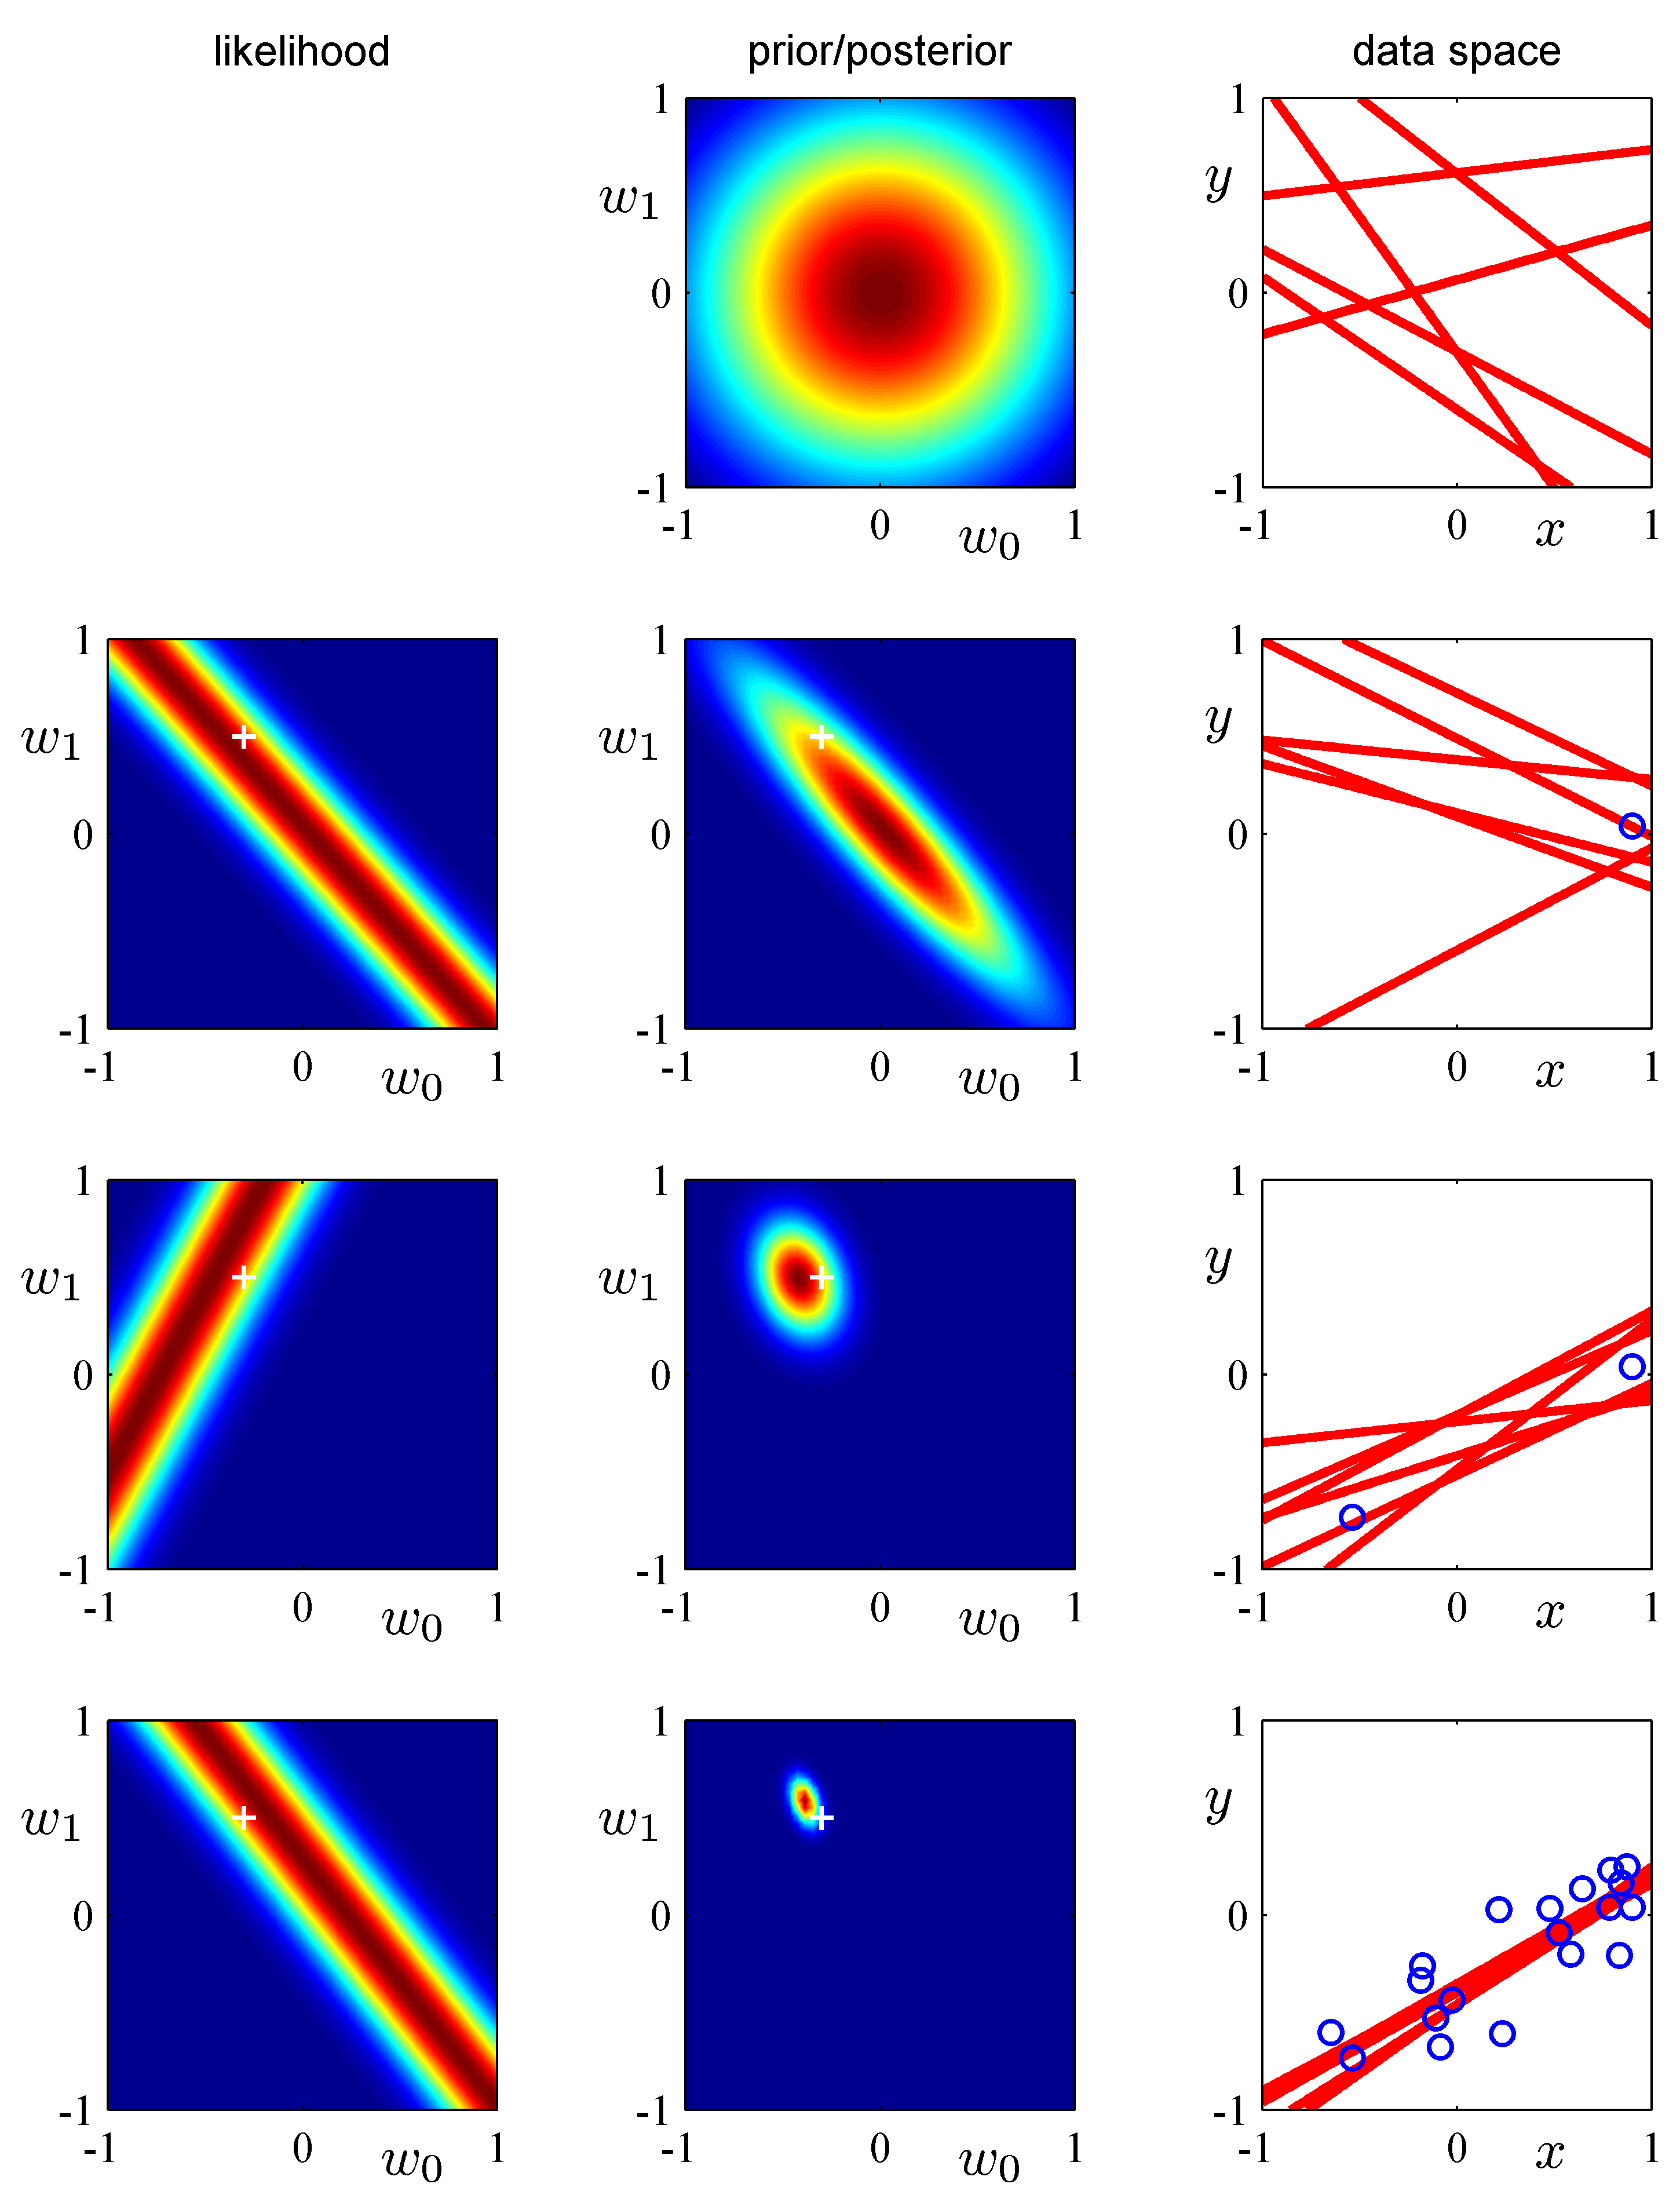
\includegraphics[scale=0.8]{Images/3-7.png}
		\captionsetup{font={small}}
		\caption{对于线性模型$y(x,\bw)=w_0+w_1 x$进行顺序贝叶斯学习的示意图。每个图像对应的具体含义请详见文字部分。}
		\label{fig:3-7}
	\end{figure}
	\indent 此外,参数的先验可以选择为另外一些形式。举例而言,可以是广义的高斯先验
	\begin{equation}
		p(\bw|\alpha) = \left[\frac{q}{2}\left(\frac{\alpha}{2}\right)^{1/q}\frac{1}{\Gamma(1/q)}\right]^M \exp \left(-\frac{\alpha}{2}\sum_{j=0}^{M-1} |w_j|^q\right)
	\end{equation}
	其中,如果$q=2$就是正常的高斯先验了,而且仅有在这种情况下,先验才与似然函数(3.10)为共轭关系。关于$\bw$求取后验分布的最大值等价于对正则化误差函数(3.29)进行最小化。对于高斯先验,后验分布的模等于均值,但如果$q \ne 2$,这条性质就不成立了。
	}
	\subsection{预测分布}
	\textnormal{
	在实际应用中,其实往往不太关心$\bw$的值,而是更关注对于$\bx$给出的预测$t$究竟如何。这就要求我们评估预测分布(predictive distribution)
	\begin{equation}
		p(t|\sft, \alpha, \beta)=\int p(t|\bw,\beta)p(\bw|\sft,\alpha,\beta)\ \mathrm{d}\bw
	\end{equation}
	其中$\sft$为训练集中的目标值向量,并省略了等号右侧条件概率中的输入向量。目标变量的条件分布$p(t|\bx, \bw, \beta)$由(3.8)给出,后验权重分布有(3.49)给出。可以看出(3.57)包含了两个高斯分布的卷积,根据第2.3.3节中的(2.115),可以看出预测分布的形式为\textcolor{red}{\textbf{—— 习题3.10}}
	\begin{equation}
		p(t|\bx, \sft, \alpha, \beta) = \calN (t|\mathbf{m}_N^{\rmT} \bfphi (\bx), \sigma_N^2 (\bx))
	\end{equation}
	其中,预测分布的方差$\sigma_N^2 (\bx)$为
	\begin{equation}
		\sigma_N^2 (\bx) = \frac{1}{\beta} + \bfphi(\bx)^{\rmT} \mathbf{S}_N \bfphi(\bx)
	\end{equation}
	(3.59)中的第1项表示数据中的噪声,第2项则表示了与$\bw$有关的不确定性。由于噪声与$\bw$的分布是相互独立的高斯分布,所以它们是可加的。需要注意的是,随着我们获取到新的数据,后验分布会变得越来越狭窄。可以证明$\sigma_{N+1}^2 (\bx) \leqslant \sigma_N^2(\bx)$(Qazaz et al., 1997)。\textcolor{red}{\textbf{—— 习题3.11}}\ 取极限$N \rightarrow \infty$,(3.59)中的第2项将趋近于0,于是预测分布的方差就只与参数$\beta$控制的噪声有关了。\\
	\indent 现在回到第1.1节中正弦数据集拟合案例中,演示一下贝叶斯线性回归模型中的预测分布。如图3.8所示,我们可以利用高斯基底函数的线性组合来构建拟合模型,而且可以随着数据集规模的变化调整拟合的方式。其中,绿色的曲线表示函数$sin(2\pi x)$,也就是真实的函数,当然是带有附加的高斯噪声的。数据点在图中用蓝色圆圈表示,当数据集的规模为$N=1,N=2,N=4,N=25$时,红色曲线表示对应的高斯预测分布的均值,红色的阴影区域表示在均值两侧加上一个标准差的范围之后得到的区域。需要注意的是,预测的不确定性取决于$x$,而且是数据点附近时取得最小值。此外,不确定性会随着数据点的增加而减小。
	\begin{figure}[H]
		\begin{minipage}[t]{0.5\linewidth}
		\centering
		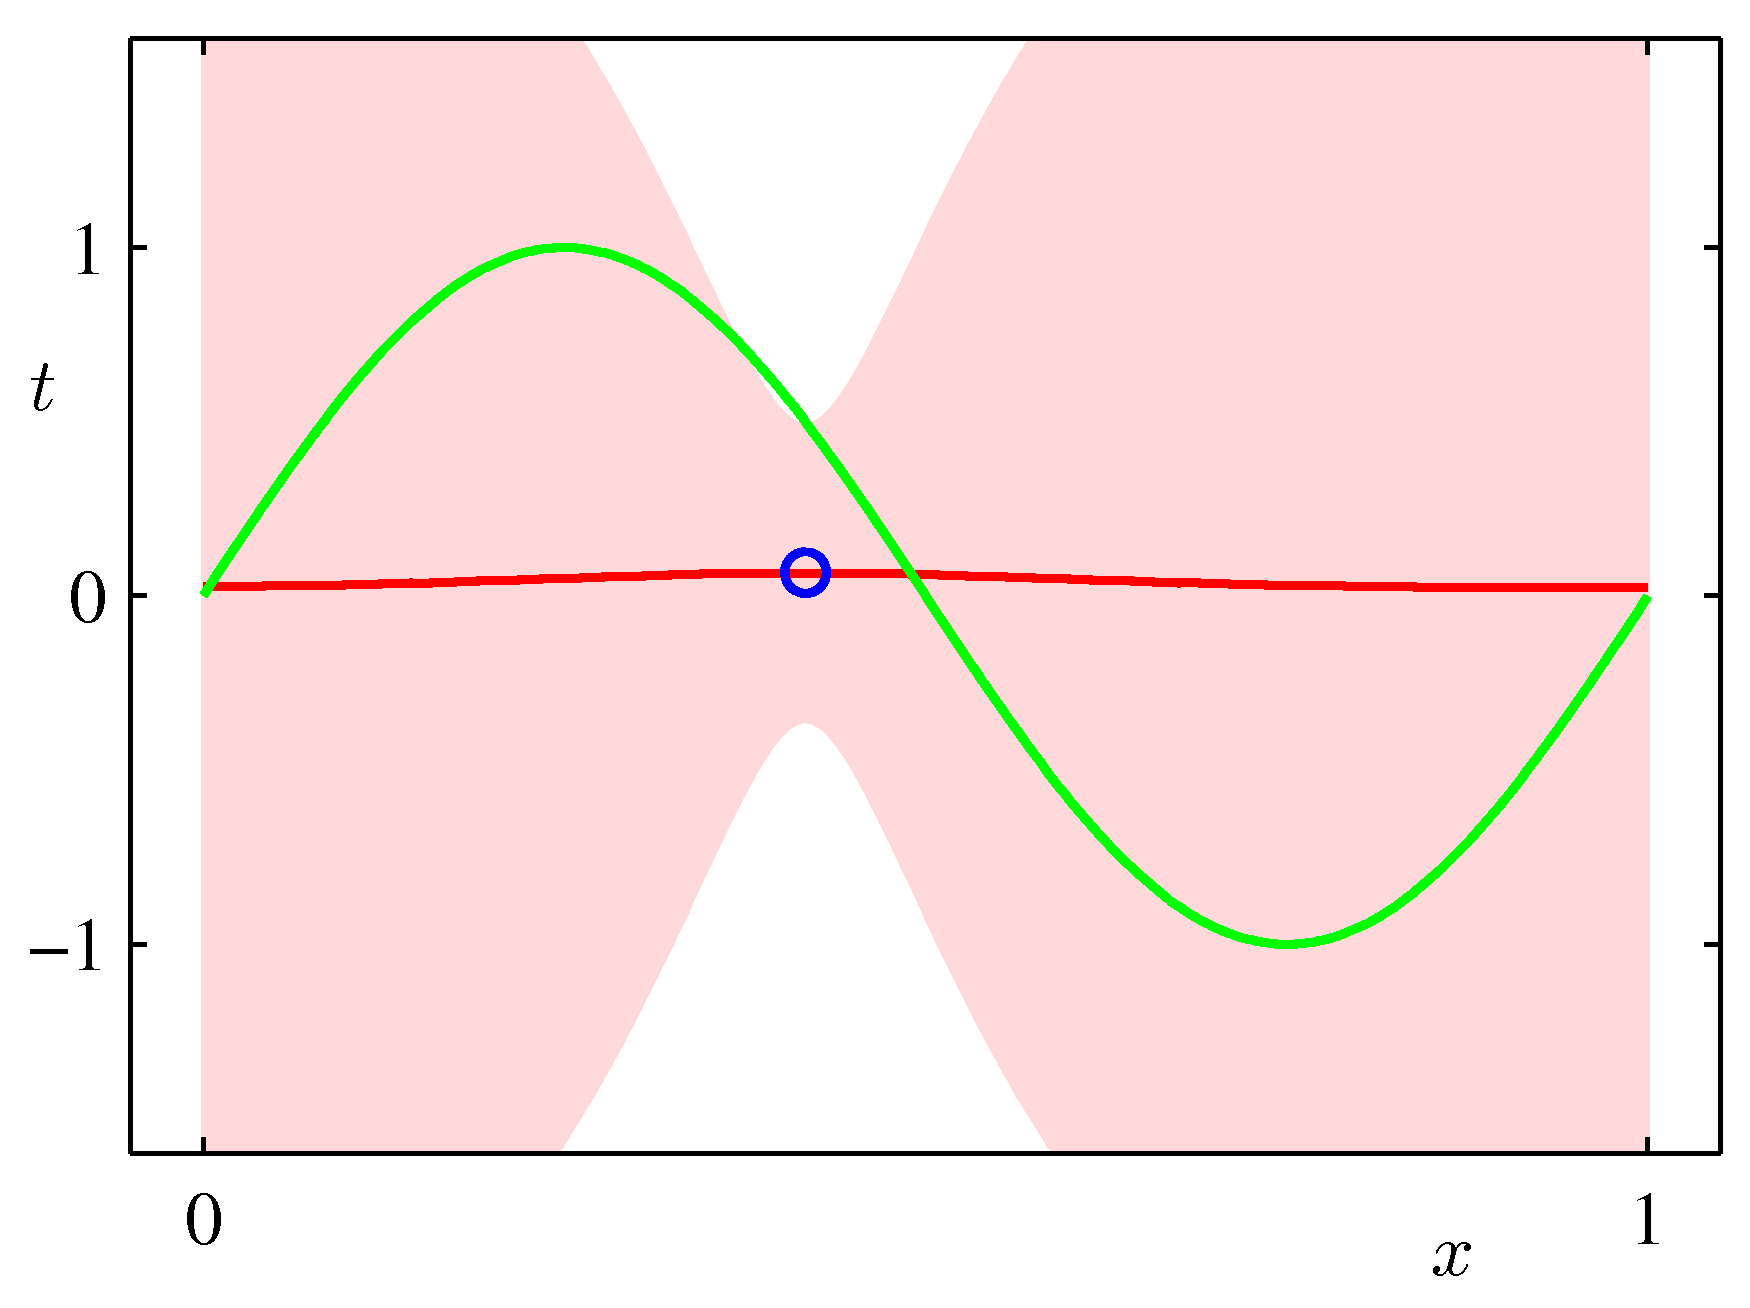
\includegraphics[scale=0.8]{Images/3-8a.png}
		\label{fig:3-8a}
		\end{minipage}
		\begin{minipage}[t]{0.5\linewidth}
		\centering
		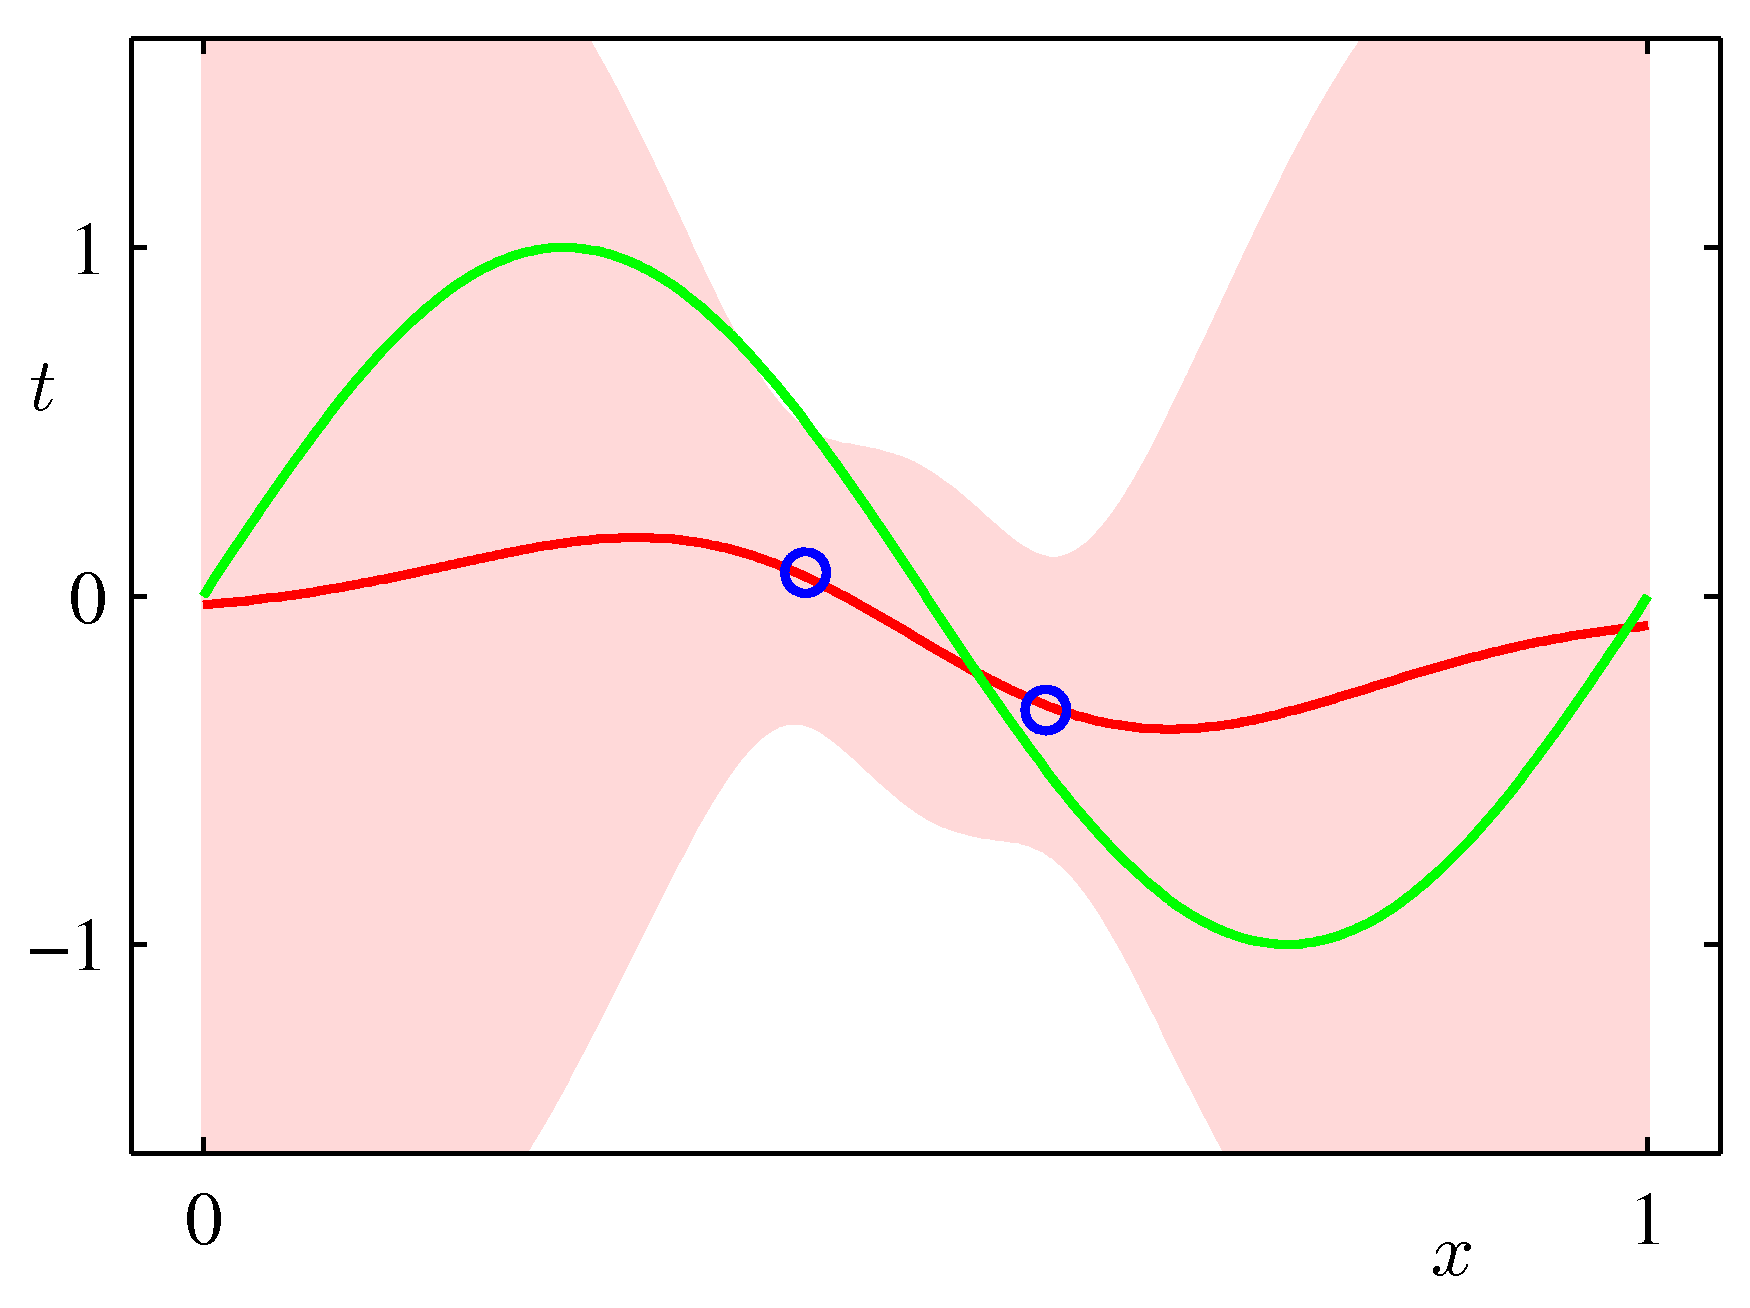
\includegraphics[scale=0.8]{Images/3-8b.png}
		\label{fig:3-8b}
		\end{minipage}\\
		\begin{minipage}[t]{0.5\linewidth}
		\centering
		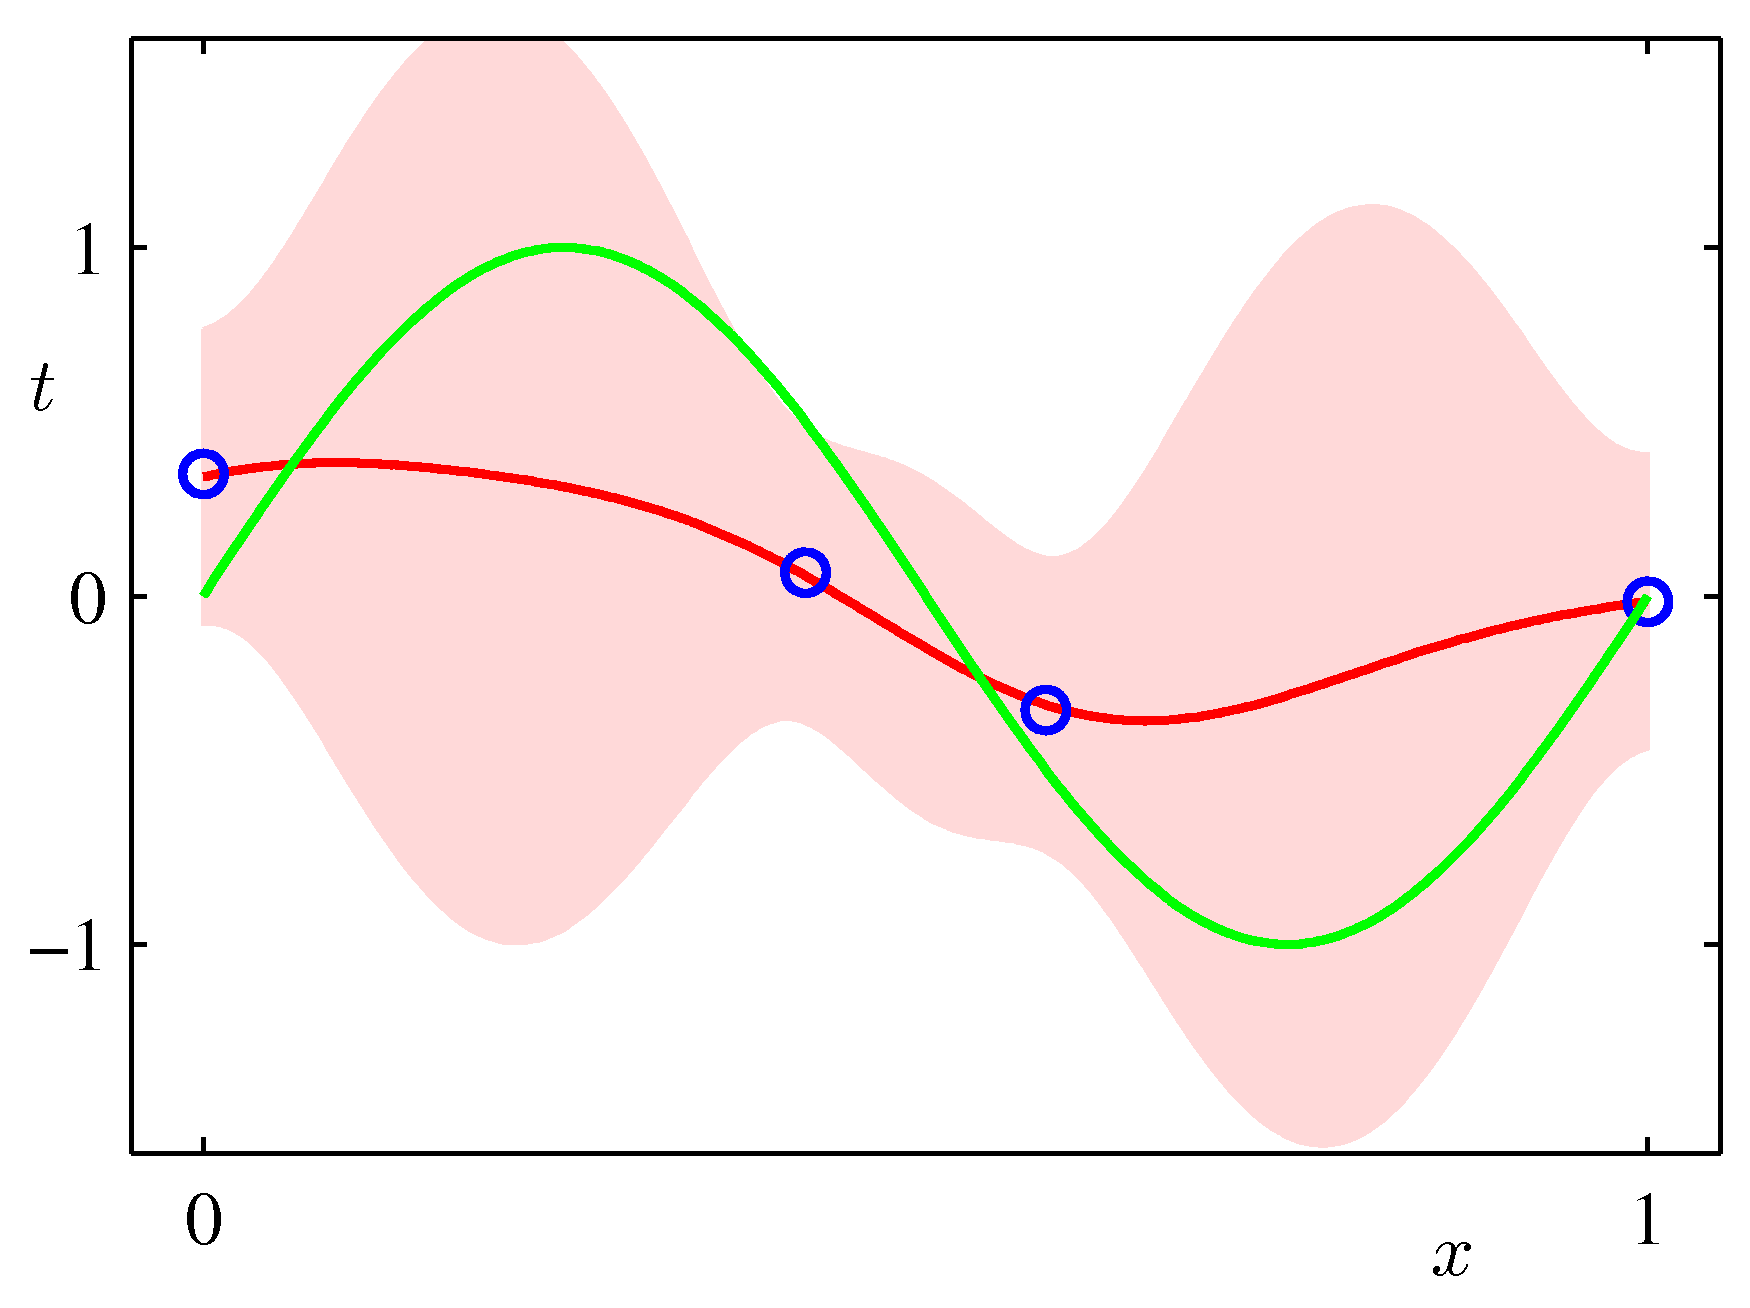
\includegraphics[scale=0.8]{Images/3-8c.png}
		\label{fig:3-8c}
		\end{minipage}
		\begin{minipage}[t]{0.5\linewidth}
		\centering
		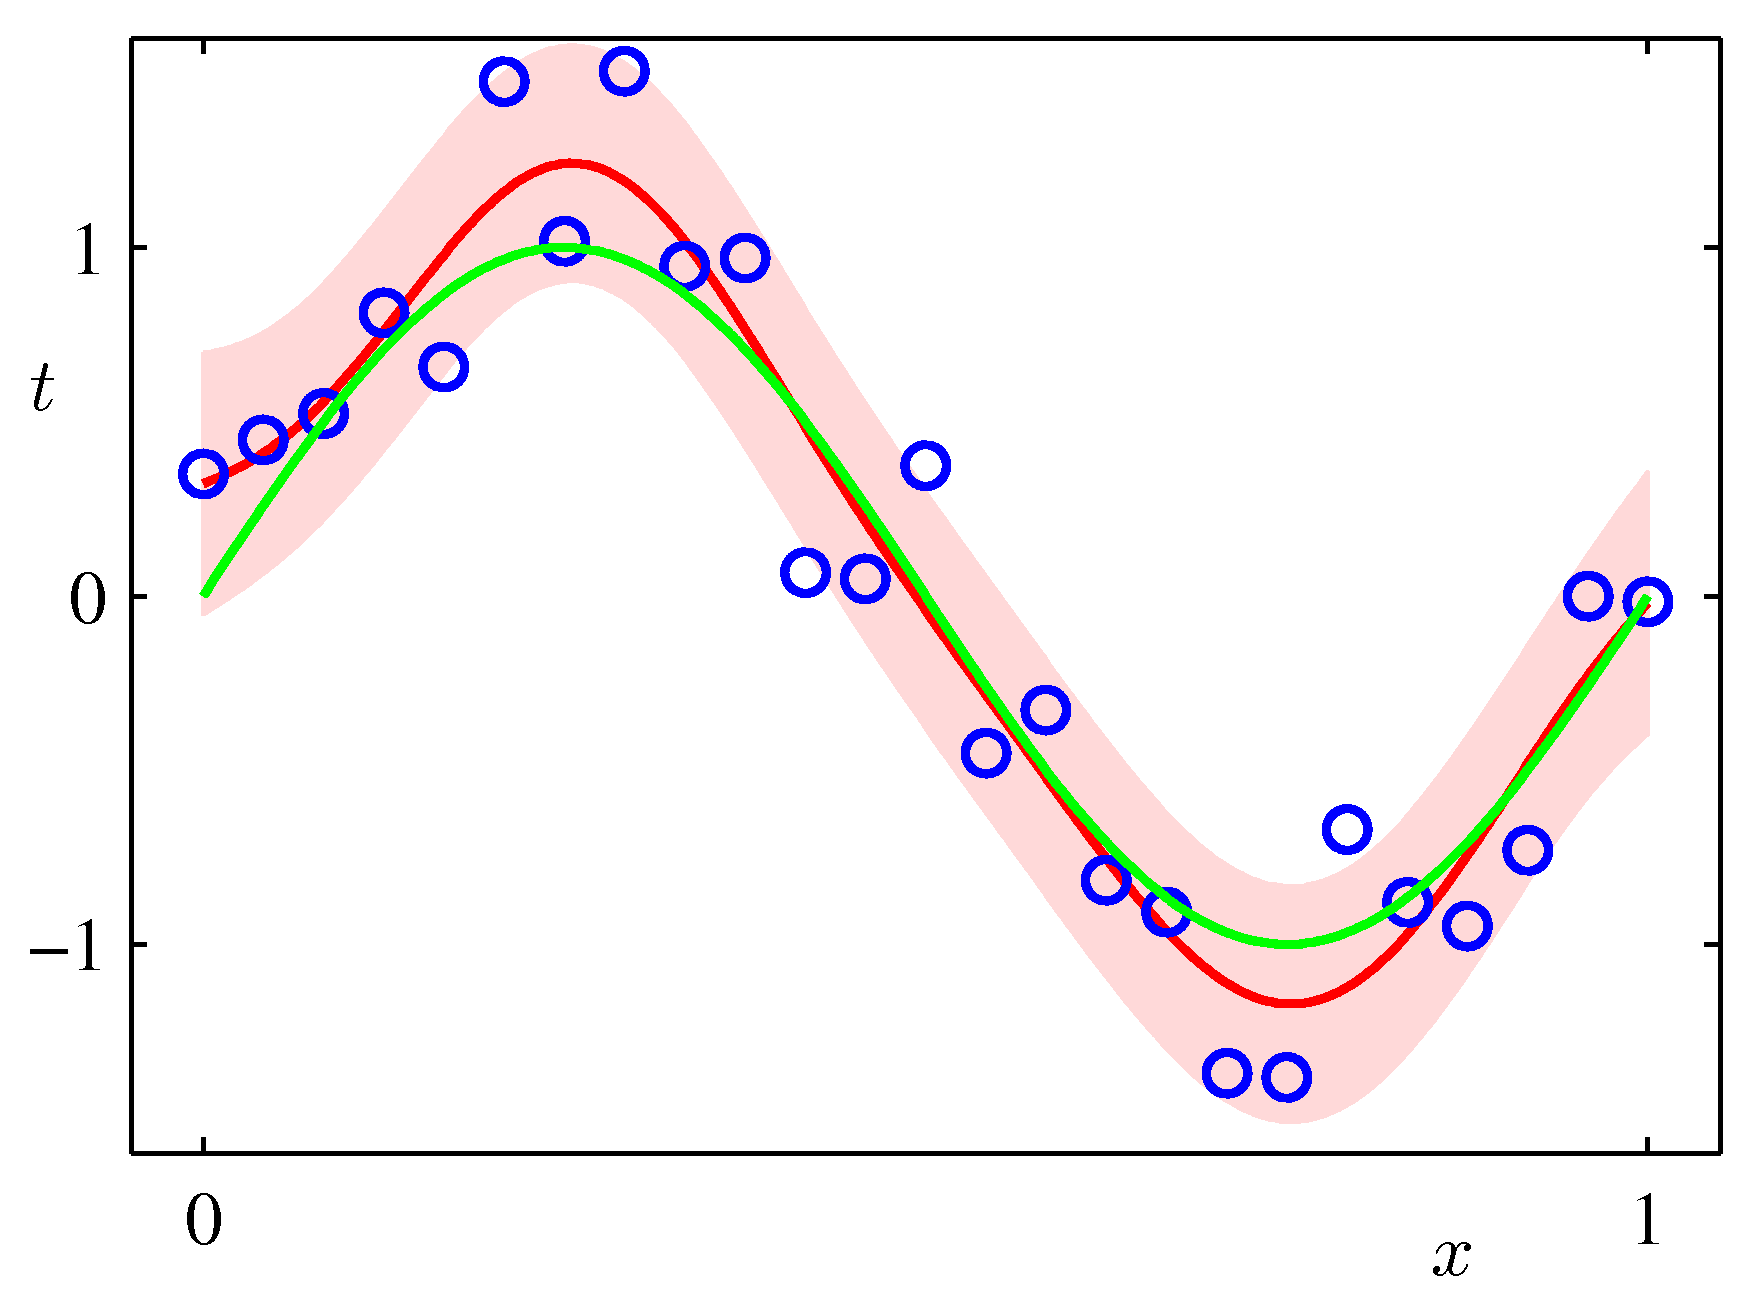
\includegraphics[scale=0.8]{Images/3-8d.png}
		\label{fig:3-8d}
		\end{minipage}
		\captionsetup{font={small}}
		\caption{根据第1.1节中的正弦函数数据集和一个包含9个高斯基底函数(3.4)的模型构建的预测分布(3.58)。具体的讨论详见正文。}
		\begin{minipage}[t]{0.5\linewidth}
		\centering
		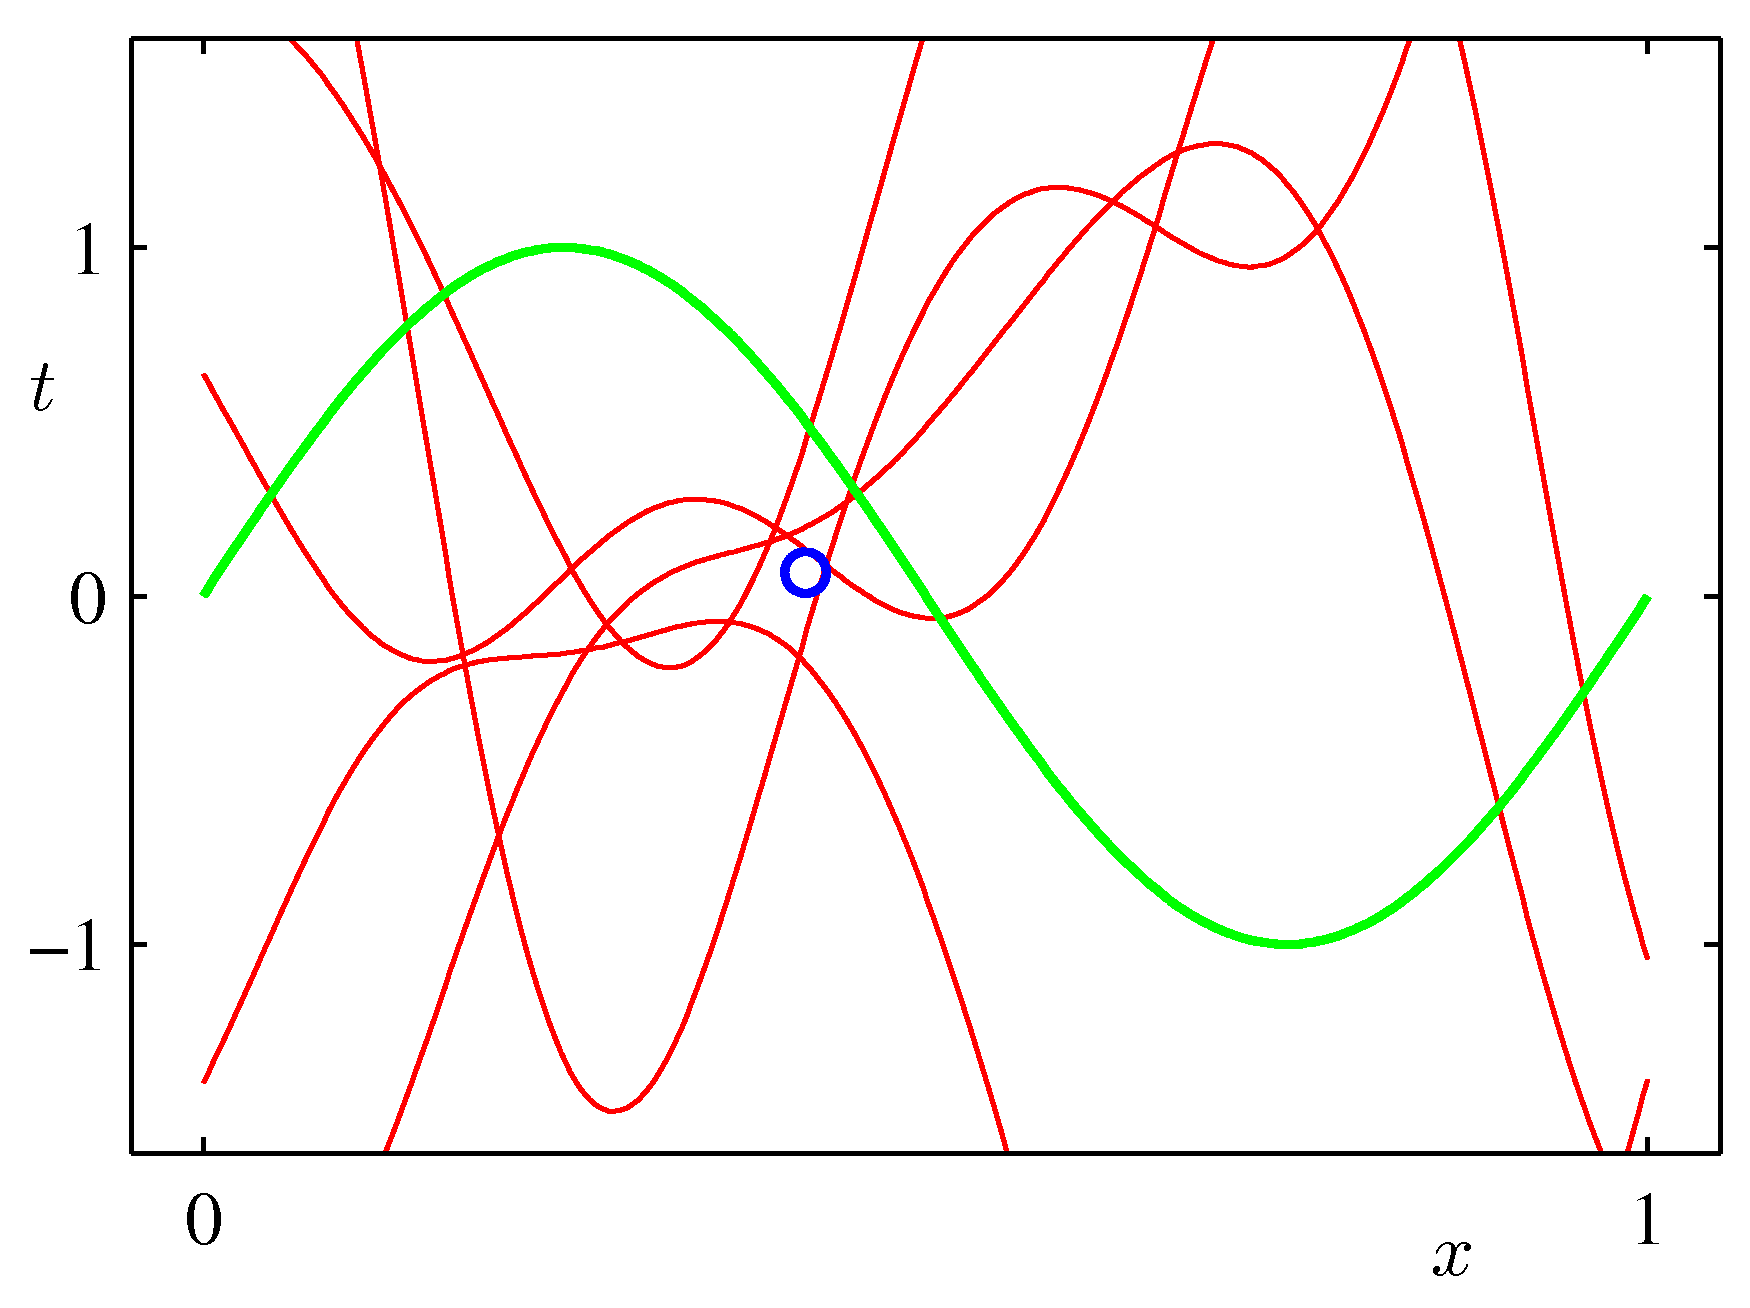
\includegraphics[scale=0.8]{Images/3-9a.png}
		\label{fig:3-9a}
		\end{minipage}
		\begin{minipage}[t]{0.5\linewidth}
		\centering
		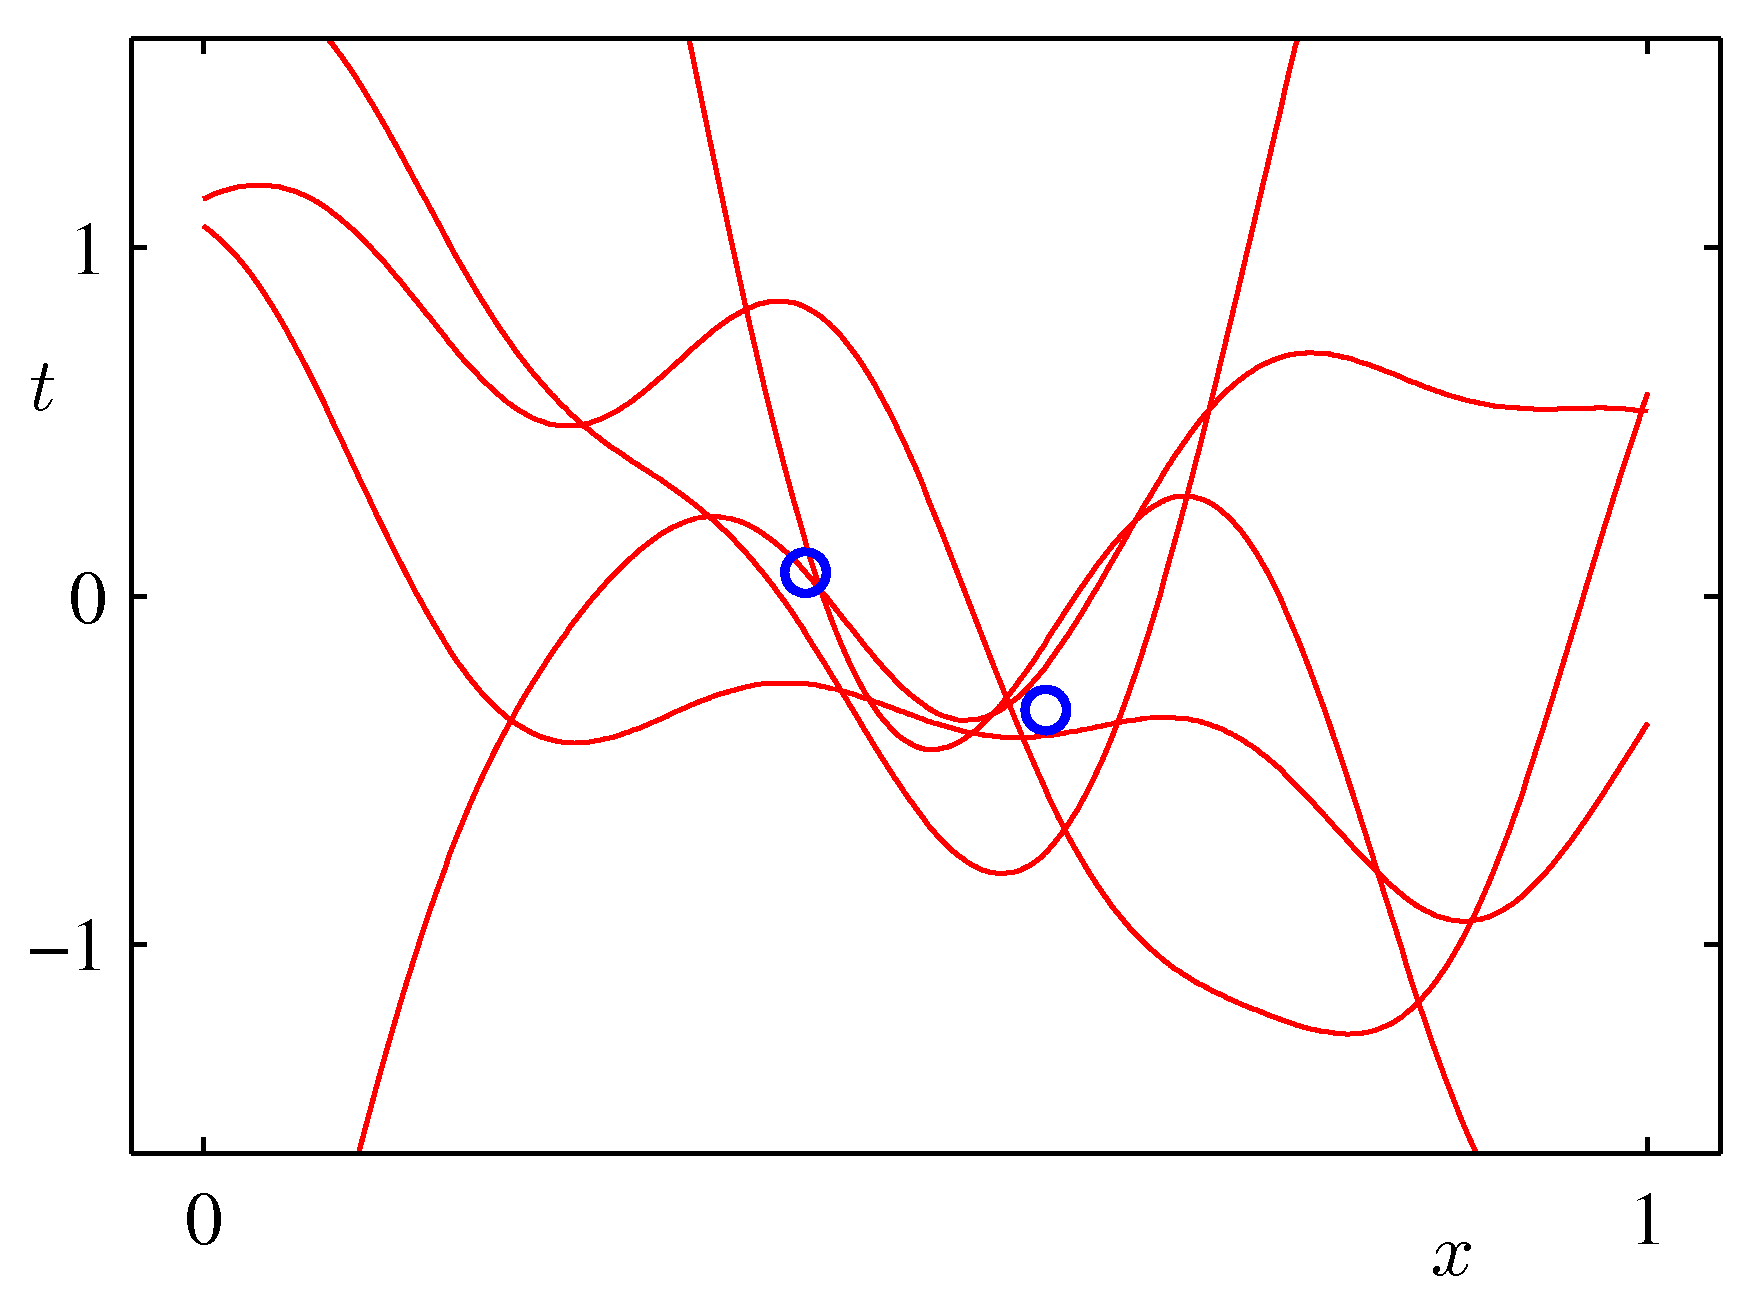
\includegraphics[scale=0.8]{Images/3-9b.png}
		\label{fig:3-9b}
		\end{minipage}\\
		\begin{minipage}[t]{0.5\linewidth}
		\centering
		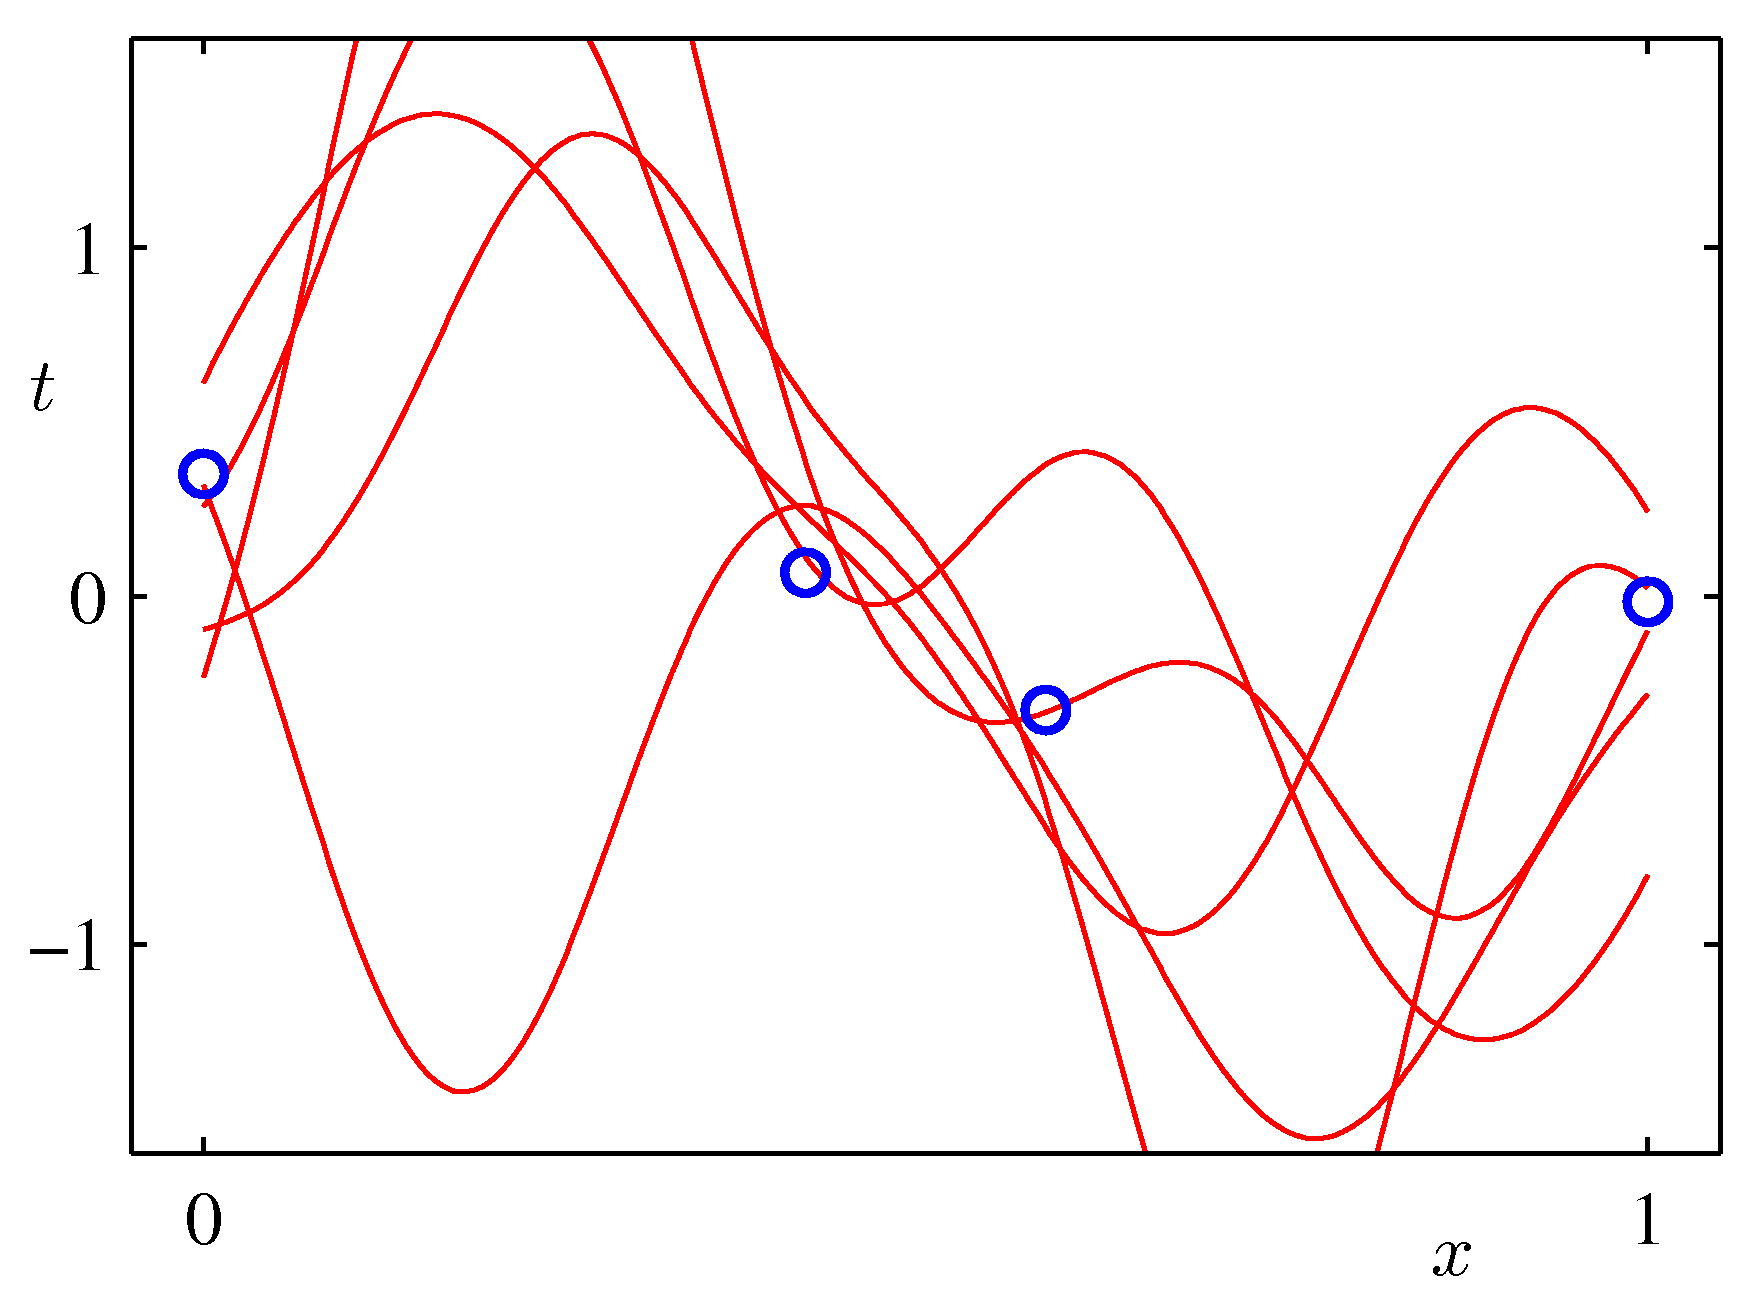
\includegraphics[scale=0.8]{Images/3-9c.png}
		\label{fig:3-9c}
		\end{minipage}
		\begin{minipage}[t]{0.5\linewidth}
		\centering
		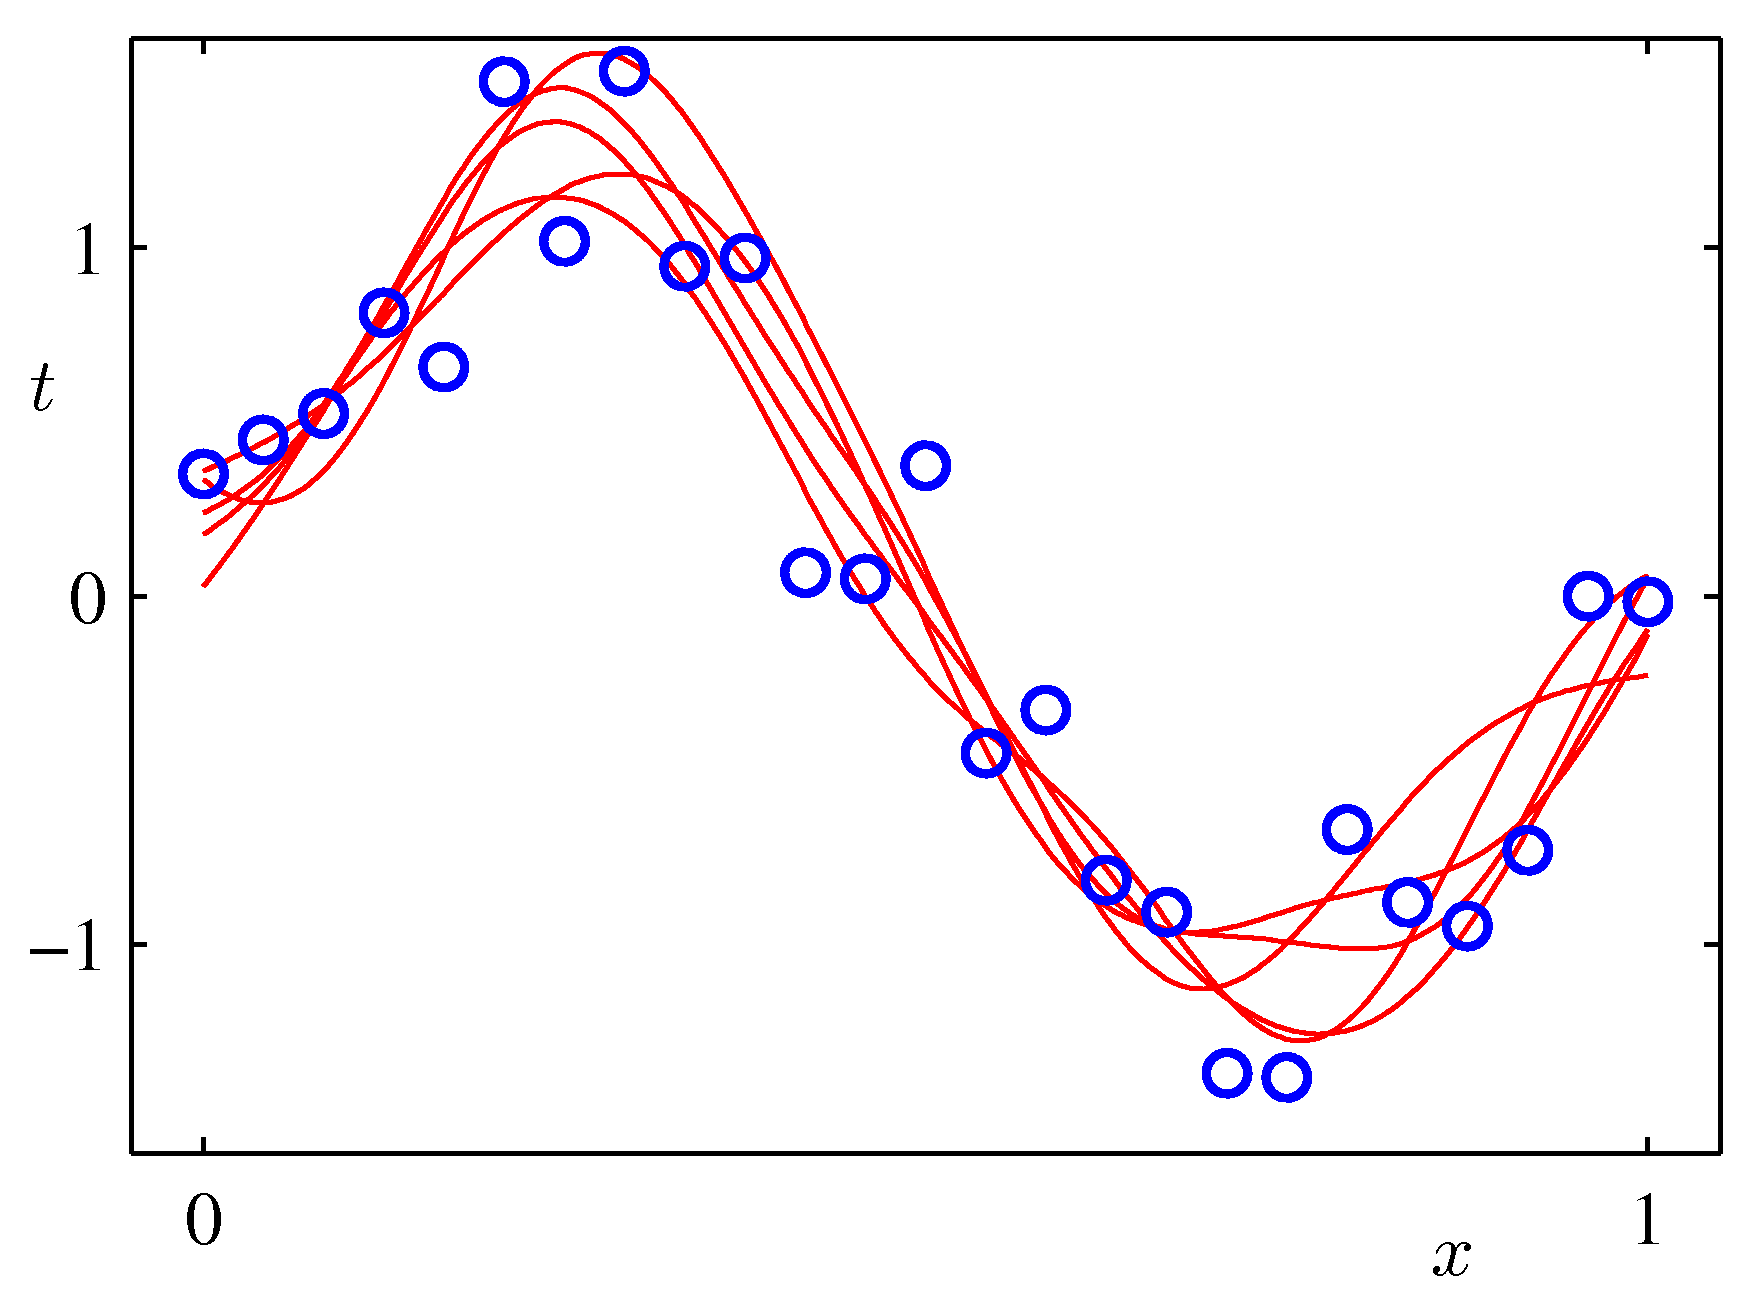
\includegraphics[scale=0.8]{Images/3-9d.png}
		\label{fig:3-9d}
		\end{minipage}
		\captionsetup{font={small}}
		\caption{从图3.8所示的分布中抽取$\bw$后画出的对应函数$y(x,\bw)$的图像。}
	\end{figure}
	\indent 图3.8中的图像仅仅展示了每个数据点处预测方差与$x$的函数关系。为了更加深刻地了解对于不同$x$进行预测时产生的协方差,我们从$\bw$的后验分布中抽取一些样本,并画出对应的函数$y(x,\bw)$,如图3.9所示。\\
	\indent 如果我们利用局部基底函数,比如局部高斯基底函数,那么在远离基底函数中心的区域,预测方差(3.59)中的第2项将趋近于0,于是只剩下了噪声造成的影响$\beta^{-1}$。所以模型对自身预测的信心将大幅增加,不过这个结果并不是什么好事。一般情况下要使用高斯过程(Gaussian process)来回避这个问题,高斯过程是另一种贝叶斯方法。\textcolor{red}{\textbf{——第6.4节}}\\
	\indent 需要注意的是,如果$\bw$和$\beta$都是未知的,那么可以先引入一个共轭先验分布$p(\bw,\beta)$,根据第2.3.6节,这是一个高斯-gamma分布(Denison et al., 2002)。\textcolor{red}{\textbf{——习题 3.12}}\ 在这种情况下,预测分布将是一个学生t分布。\textcolor{red}{\textbf{—— 习题3.13}}
	}
	\subsection{等价核}
	\textnormal{
	线性基底函数模型的后验均值解(3.53)有一个奇妙的解释,而且这种解释可以为接下来的核方法(kernel method)铺路,核方法中有一项就是高斯过程。\textcolor{red}{\textbf{——第6章}}\ 如果将(3.53)代入到(3.3)中,可以看出预测均值的形式为
	\begin{equation}
		y(\bx, m_N) = \mathbf{m}_N^{\rmT}\bfphi(\bx) = \beta \bfphi(\bx)^{\rmT} \mathbf{S}_N \bfPhi^{\rmT}\sft = \sum_{n=1}^N \beta \bfphi(\bx)^{\rmT} \mathbf{S}_N \bfphi(\bx_n)t_n
	\end{equation}
	其中$\mathbf{S}_N$就是(3.51)定义的那个。所以在$\bx$处预测分布的均值就变成了训练集目标变量$t_n$的线性组合,于是
	\begin{equation}
		y(\bx,\mathbf{m}_N) = \sum_{n=1}^N k(\bx, \bx_n)t_n
	\end{equation}
	其中函数
	\begin{equation}
		k(\bx, \bx')=\beta \bfphi(\bx)^{\rmT} \mathbf{S}_N\bfphi(\bx ')
	\end{equation}
	称为平滑矩阵(smoother matrix)或等价核(equivalent kernel)。类似这样的可以通过训练集的目标变量值进行预测的回归函数称为线性平滑器(linear smoother)。需要注意的是,等价核依赖于输入量$\bx_n$,因为它们在$\mathbf{S}_N$中出现了。如图3.10所示的是以高斯基底函数为例的等价核,其中将核函数$k(x,x')$画成了3种不同$x$取值下关于$x'$的函数。可以看出曲线一直在$x$附近波动,所以在$x$处预测分布的均值$y(x,\mathbf{m}_N)$就可以通过构建目标变量的加权线性组合来确定,其中,距离$x$较近的数据点会被赋予较高的权重,反之亦然。从直觉上来说这似乎是挺合理的,毕竟远亲不如近邻【虽然这话放在这好像不很贴切,就那么回事吧】。需要注意的是,这个性质不仅适用于局部高斯基底函数,而是同样适用于非局部多项式和sigmoid基底函数,如图3.11所示。
	\begin{figure}[ht]
		\centering
		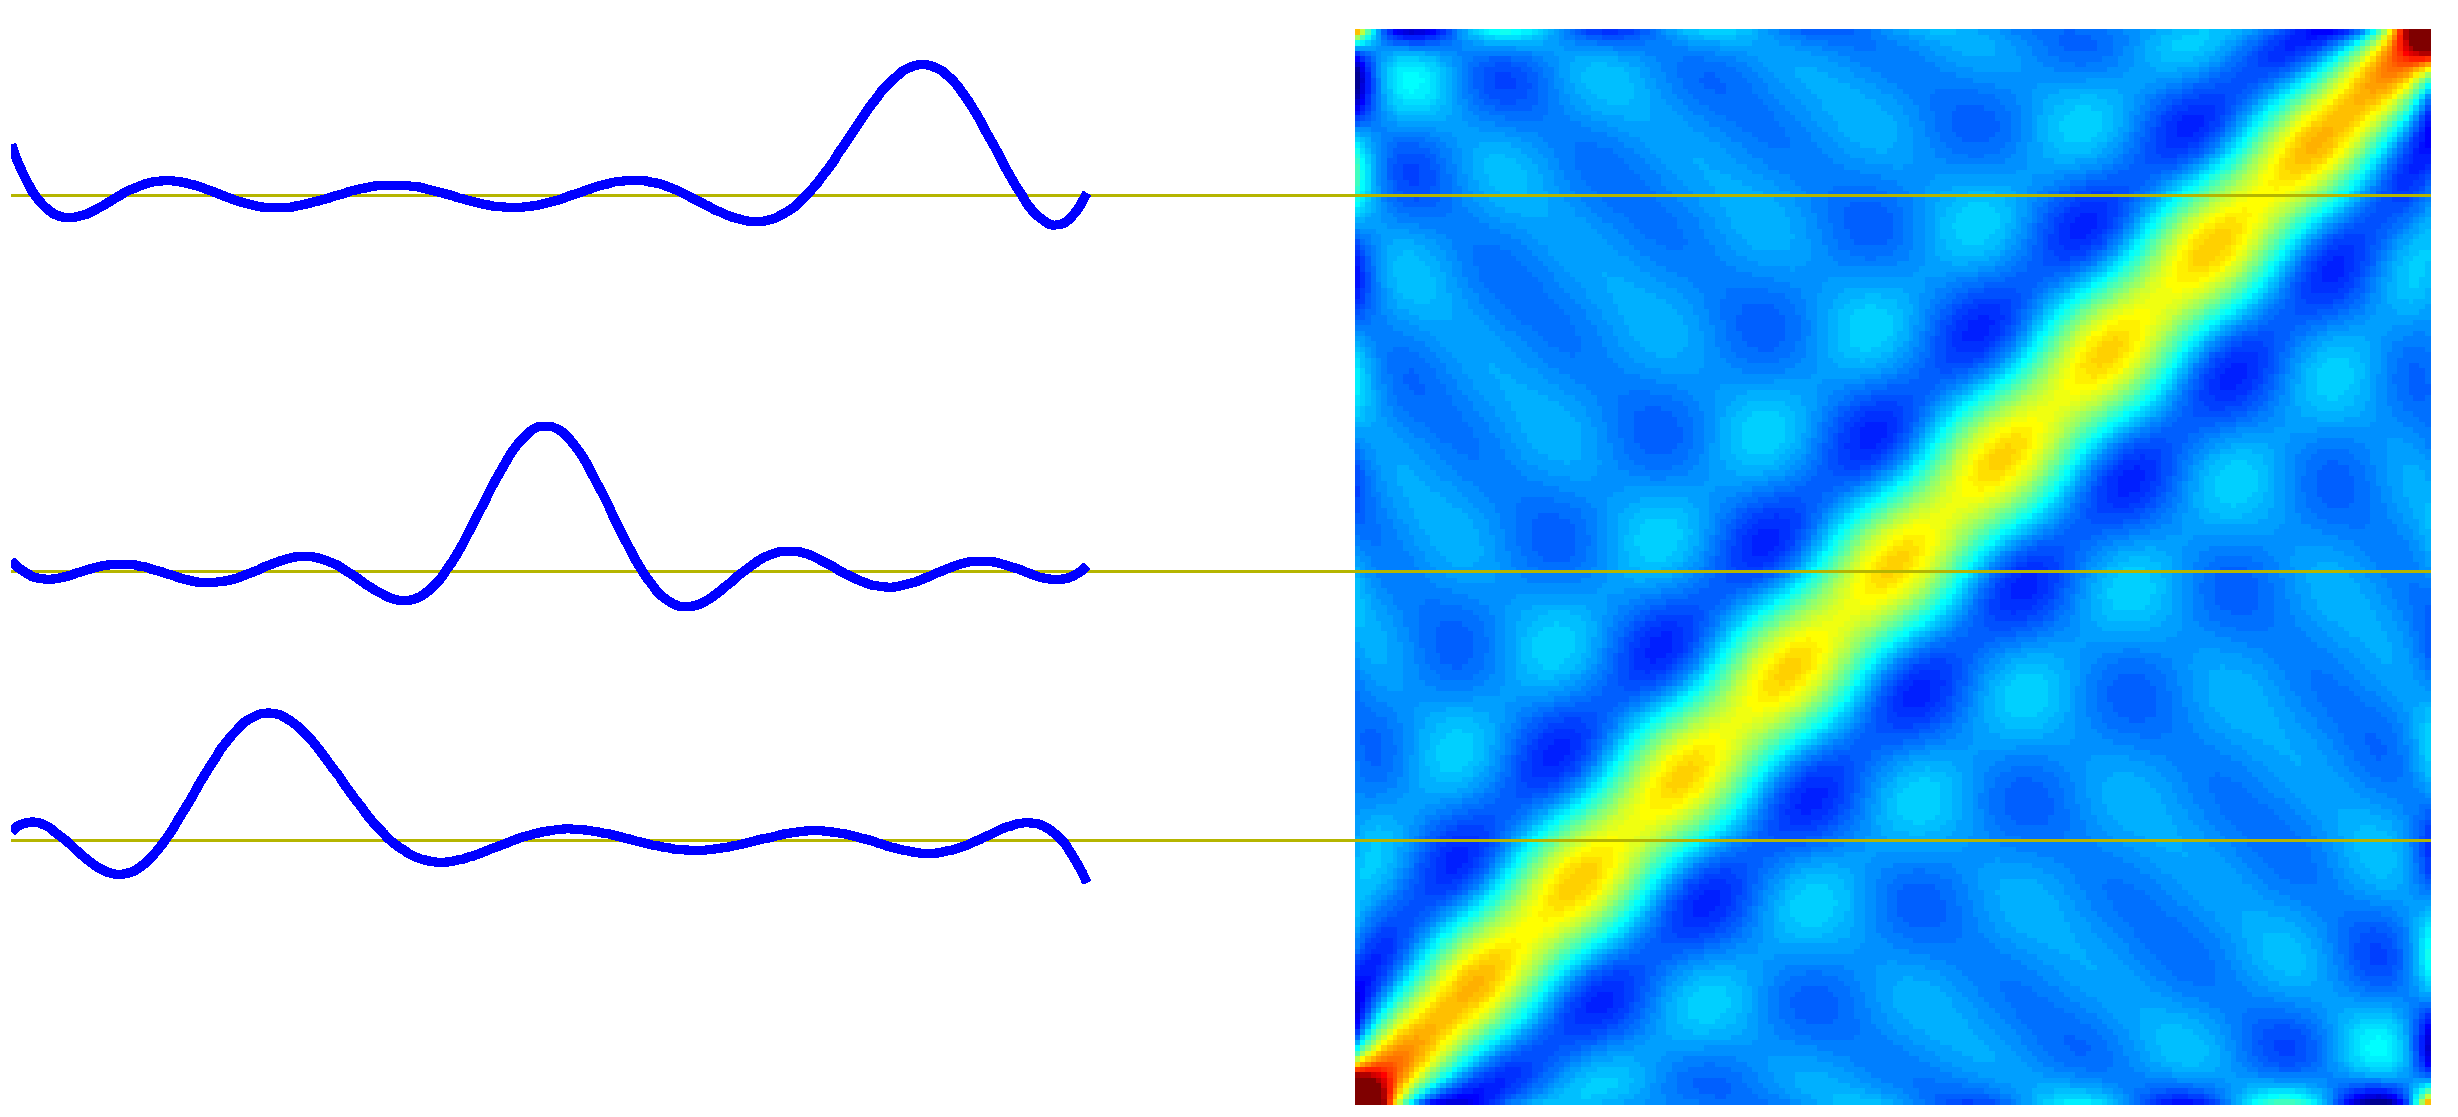
\includegraphics[scale=0.8]{Images/3-10.png}
		\captionsetup{font={small}}
		\caption{图3.1中的高斯基底函数的等价核$k(x,x')$,在这里画成了$x-x'$的形式,同时给出了该矩阵的3个不同$x$取值处的具体情况。生成这个核所用的数据$x$是从$(-1,1)$之间均匀取出的200个值。}
		\label{fig:3-10}
	\end{figure}
	\begin{figure}[ht]
		\begin{minipage}[t]{0.5\linewidth}
		\centering
		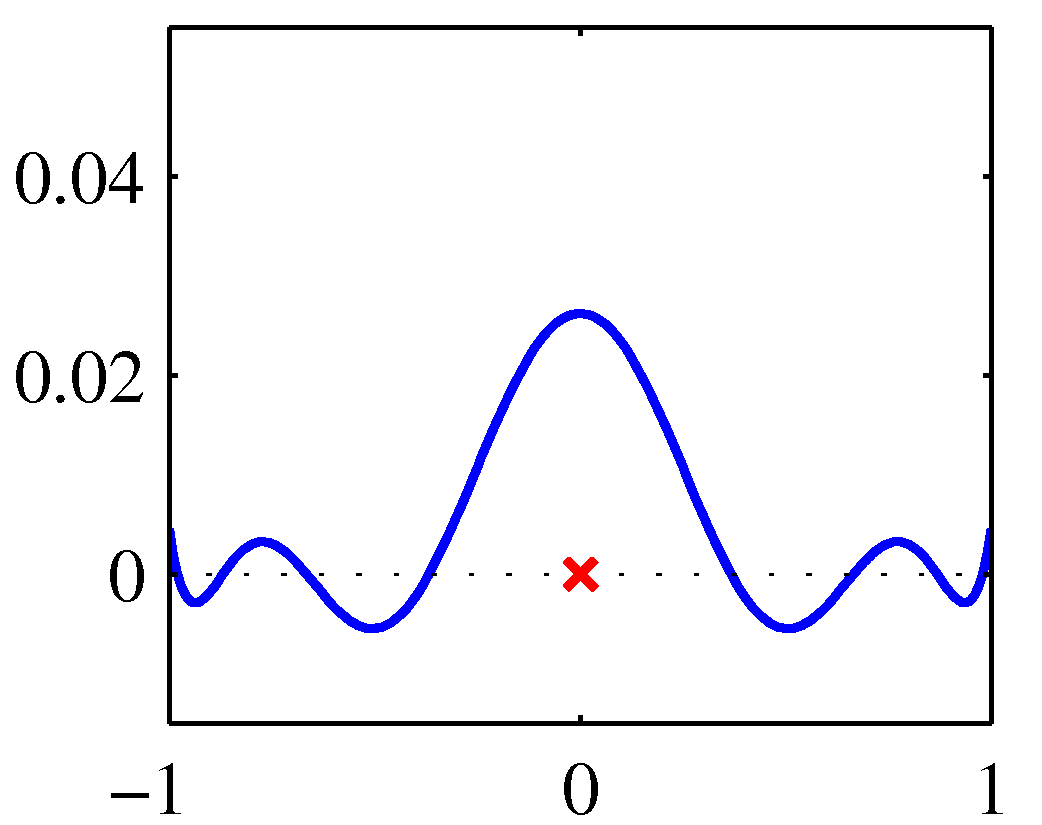
\includegraphics[scale=0.8]{Images/3-11a.png}
		\label{fig:3-11a}
		\end{minipage}
		\begin{minipage}[t]{0.5\linewidth}
		\centering
		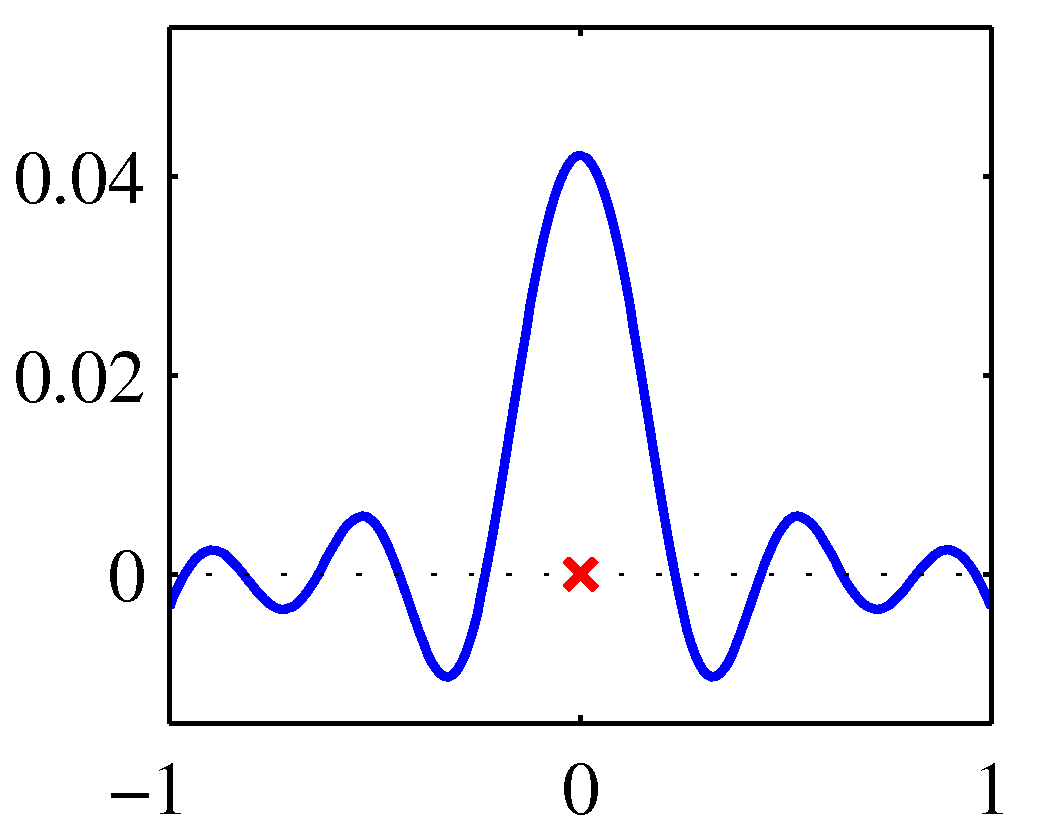
\includegraphics[scale=0.8]{Images/3-11b.png}
		\label{fig:3-11b}
		\end{minipage}
		\captionsetup{font={small}}
		\caption{$x=0$时的等价核,这里画成了$x$的函数的形式,左侧为多项式基底函数,右侧为sigmoid基底函数。需要注意的是,尽管它们对应的基底函数并非是局部的,它们也是关于$x$的局部函数。}
	\end{figure}
	\\
	\indent 关于等价核这个问题,可以通过研究$y(\bx)$与$y(\bx')$之间的协方差来获取更进一步的认知。这个协方差为
	\begin{equation}
	\begin{split}
		\mathrm{cov} [y(\bx),y(\bx')] &= \mathrm{cov}\left[\bfphi(\bx)^{\rmT} \bw, \bw^{\rmT}\bfphi(\bx')\right]\\
		&= \bfphi(\bx)^{\rmT}\mathbf{S}_N\bfphi(\bx') = \beta^{-1}k(\bx,\bx')
	\end{split}
	\end{equation}
	其中用到了(3.49)和(3.62)。从等价核的形式可以看出,距离较近的点也具有较强的相关性,而距离较远的点则相反。\\
	\indent 图3.8中的预测分布使得我们可以看到预测中每个点的不确定性,这里的不确定性是由(3.59)确定的。通过从后验分布中抽取一些$\bw$的样本,并画出图3.9这样的对应模型函数$y(\bx,\bw)$,我们可以看到后验分布中$y$值与两个(或多个)$x$值之间的联合不确定性,这个不确定性是由等价核确定的。\\
	\indent 核函数形式的线性回归提出了如下的求解回归问题的替代方法。这里并不需要扯进一大堆基底函数,因为基底函数实际上也构建了一个等价核,而是要直接定义一个局部核,并用它来对新的输入$\bx$做预测,当然是建立在一个训练集的基础上了。这个做法构建了一种求解回归问题(或分类问题)方法的重要框架,这个方法称为高斯过程,具体内容详见第6.4节。\\
	\indent 我们已经看到等价核根据训练集中的目标变量值定义了权重,从而对新的$\bx$做出预测,而且这些权重的总和一定为1,即\textcolor{red}{\textbf{——习题 3.14}}
	\begin{equation}
		\sum_{n=1}^N k(\bx,\bx_n) = 1
	\end{equation}
	这个结果引发强烈的舒适,如果不想太正式地证明,也可以用如下方法:这个求和等价于对一个$t_n$全部等于1的数据集求预测均值$\hat{y}(\bx)$。由于基底函数都是线性无关的,所以数据的数量一定大于基底函数的数量,而且一定有一个基底函数是常数(这样才有和偏差参数对应的基底函数),那就一定可以对训练数据进行拟合,而且预测均值一定是$\hat{y}(\bx)=1$,于是就得到了(3.64)。需要注意的是,核函数可正可负,所以尽管它们满足上述的总和约束,但对应的预测并不一定是训练集中目标变量的凸组合。\\
	\indent 最后还有点事情需要注意,等价核(3.62)满足一个一般的核函数都满足的重要性质,即它们可以写成非线性函数$\boldsymbol{\psi}(\bx)$内积的形式:\textcolor{red}{\textbf{——第6章}}
	\begin{equation}
		k(\bx,\mathbf{z}) = \boldsymbol{\psi}(\bx)^{\rmT} \boldsymbol{\psi}(\mathbf{z})
	\end{equation}
	其中$\boldsymbol{\psi}(\bx)=\beta^{1/2}\mathbf{S}_N^{1/2}\bfphi(\bx)$。
	}
	\section{贝叶斯模型的对比}
	\insertline\\
	\textnormal{
	\indent 在第1章中我们曾强调了过拟合这个问题,并提出利用交叉验证方法来设定正则项参数或进行模型的选择。选择我们研究一下贝叶斯视角下的模型选择问题。在这一节中,我们所进行的讨论会比较针对一般情况,在第3.5节中我们再集中精力去解决在线性回归中确定正则化参数的问题。\\
	\indent 我们即将开拿到,最大似然方法中的过拟合问题可以通过对模型参数进行边缘化(离散变量是求和,连续变量是积分)来解决,相比之下,点估计的方法则很容易出问题。模型的比较可以直接在训练集上进行,而不需要独立的验证集。这就使得所有的数据都可以用于训练,而且避免了交叉验证的问题——毕竟交叉验证要多次训练,很是麻烦。而且这样的方法还可以在训练过程中顺便同时确定复杂度参数。举个例子,在第7章中我们会介绍相关向量机(relevance vector machine),这是一个典型的贝叶斯模型,对每组训练数据都有一个复杂度参数。\\
	\indent 贝叶斯视角下的模型对比仍然是使用概率来表示模型选择的不确定性,当然,加法规则和乘法规则是必不可少的。假设希望比较的模型组成了一个规模为$L$的模型集合$\{\mathcal{M}_i\}$,其中$i=1,...,L$。这里的模型指的是观测数据$\calD$上的概率分布。在多项式曲线拟合问题中,这个分布就是建立在目标变量集合$\sft$上的,并认为输入变量集合$\mathbf{X}$是已知的。另一种模型是$\mathbf{X}$和$\sft$的联合分布。\textcolor{red}{\textbf{——第1.5.4节}}\ 我们假设数据是从其中的某一个模型中获取的,但又不确定究竟是哪一个。不确定性是通过先验概率分布$p(\mathcal{M}_i)$来表示的。在给定了训练集$\calD$的条件下,接下来我们希望评价后验分布
	\begin{equation}
		p(\mathcal{M}_i|\calD) \propto p(\mathcal{M}_i)p(\calD|\mathcal{M}_i)
	\end{equation}
	先验表示我们对不同模型的偏好程度。现在先假设所有模型的先验概率都是一样的。其实最主要的部分是模型证据(model evidence)$p(\calD|\mathcal{M}_i)$,这一项表示的是数据对不同模型所表现出来的"偏好程度",接下来更加深入地聊聊这个问题。模型证据有时候也被称为边缘似然(marginal likelihood),因为它可以被视为是一个模型空间中的似然函数,在这个"似然函数"中,所有的参数都已经被边缘化掉了。两个模型的模型证据的比值$p(\calD|\mathcal{M}_i)/p(\calD|\mathcal{M}_j)$称为贝叶斯因子(Bayesian factor, Kass and Raftery, 1995)。\\
	\indent 模型的后验分布一旦确定,那么根据加法规则和乘法规则,预测分布为
	\begin{equation}
		p(t|\bx,\calD) = \sum_{i=1}^L p(t|\bx,\mathcal{M}_i, \calD)p(\mathcal{M}_i|\calD)
	\end{equation}
	这是一个混合分布(mixture distribution),其中,通过对预测分布$p(t|\bx,\mathcal{M}_i, \calD)$求加权平均值,且权重为每个模型各自的后验概率$p(\mathcal{M}_i|\calD)$,从而确定最终的整体预测分布。举例而言,假设有两个模型,这两个模型的后验概率相同,一个是在$t=a$附近,另一个在$t=b$附近,那么最终的整体预测分布就是一个双峰分布,一个峰位于$t=a$,另一个位于$t=b$,而非一个$t=(a+b)/2$的单峰分布。\\
	\indent 对模型取平均值有一个简单的近似方法,那就是直接将可能性最大的模型作为最终结果,这个问题就是模型选择(model selection)问题。\\
	\indent 对于一个由参数$\bw$控制的模型,根据加法规则和乘法规则,模型证据为
	\begin{equation}
		p(\calD|\mathcal{M}_i)=\int p(\calD|\bw, \mathcal{M}_i)p(\bw|\mathcal{M}_i)\ \mathrm{d}\bw
	\end{equation}
	从采样方法的角度来看,\textcolor{red}{\textbf{——第11章}}\ 边缘似然可以看成是能够从模型中得到数据集$\calD$的概率,而参数则是从先验中随机抽取出来的。另一方面,"证据"恰好又是估计参数的后验分布时贝叶斯定理分母中的归一化项。因为
	\begin{equation}
		p(\bw|\calD,\mathcal{M}_i) = \frac{p(\calD|\bw,\mathcal{M}_i) p(\bw|\mathcal{M}_i)}{p(\calD|\mathcal{M}_i)}
	\end{equation}
	\indent 我们可以通过对参数的积分进行一个简单的近似,从而更加深刻地认识模型证据的含义。假设模型仅有一个参数$w$。参数的后验分布是与$p(\calD|w)p(w)$成正比的,其中忽略了依赖项中的$\mathcal{M}_i$从而简化符号。如果我们假设后验分布是一个在最大似然值$w_{\mathrm{MAP}}$处的尖峰,其宽度为$\Delta w_{\mathrm{posterior}}$,于是就可以将积分进行近似为被积函数的函数值与尖峰宽度的乘积。如果进一步假设先验分布是平坦的,且宽度为$\Delta w_{\mathrm{prior}}$,那么$p(w)=1/\Delta w_{\mathrm{prior}}$,于是
	\begin{equation}
		p(\mathcal{D})= \int p(\calD|w)p(w)\ \mathrm{d}w \approx p(\calD|w_{\mathrm{MAP}})\frac{\Delta w_{\mathrm{posterior}}}{\mathrm{\Delta w_{\mathrm{prior}}}}
	\end{equation}
	对两侧同时取对数,则有
	\begin{equation}
		\ln p(\calD) \approx \ln p(\calD|w_{\mathrm{MAP}})+\ln \left(\frac{\Delta w_{\mathrm{posterior}}}{\Delta w_{\mathrm{prior}}}\right)
	\end{equation}
	这个近似的过程如图3.12所示。第1项表示的是概率最大的参数值给出的数据拟合结果,对于一个平坦先验分布而言,与之对应的就是对数似然。第二项根据模型的复杂度进行模型惩罚。由于$\Delta w_{\mathrm{posterior}} < \Delta w_{\mathrm{prior}}$,所以这一项是负值,而且随着这个比值的减小,其绝对值会增加。所以,如果取得某种参数下的后验分布对数据的拟合效果非常好,那么惩罚项也会相应变得非常大。
	\begin{figure}[ht]
		\centering
		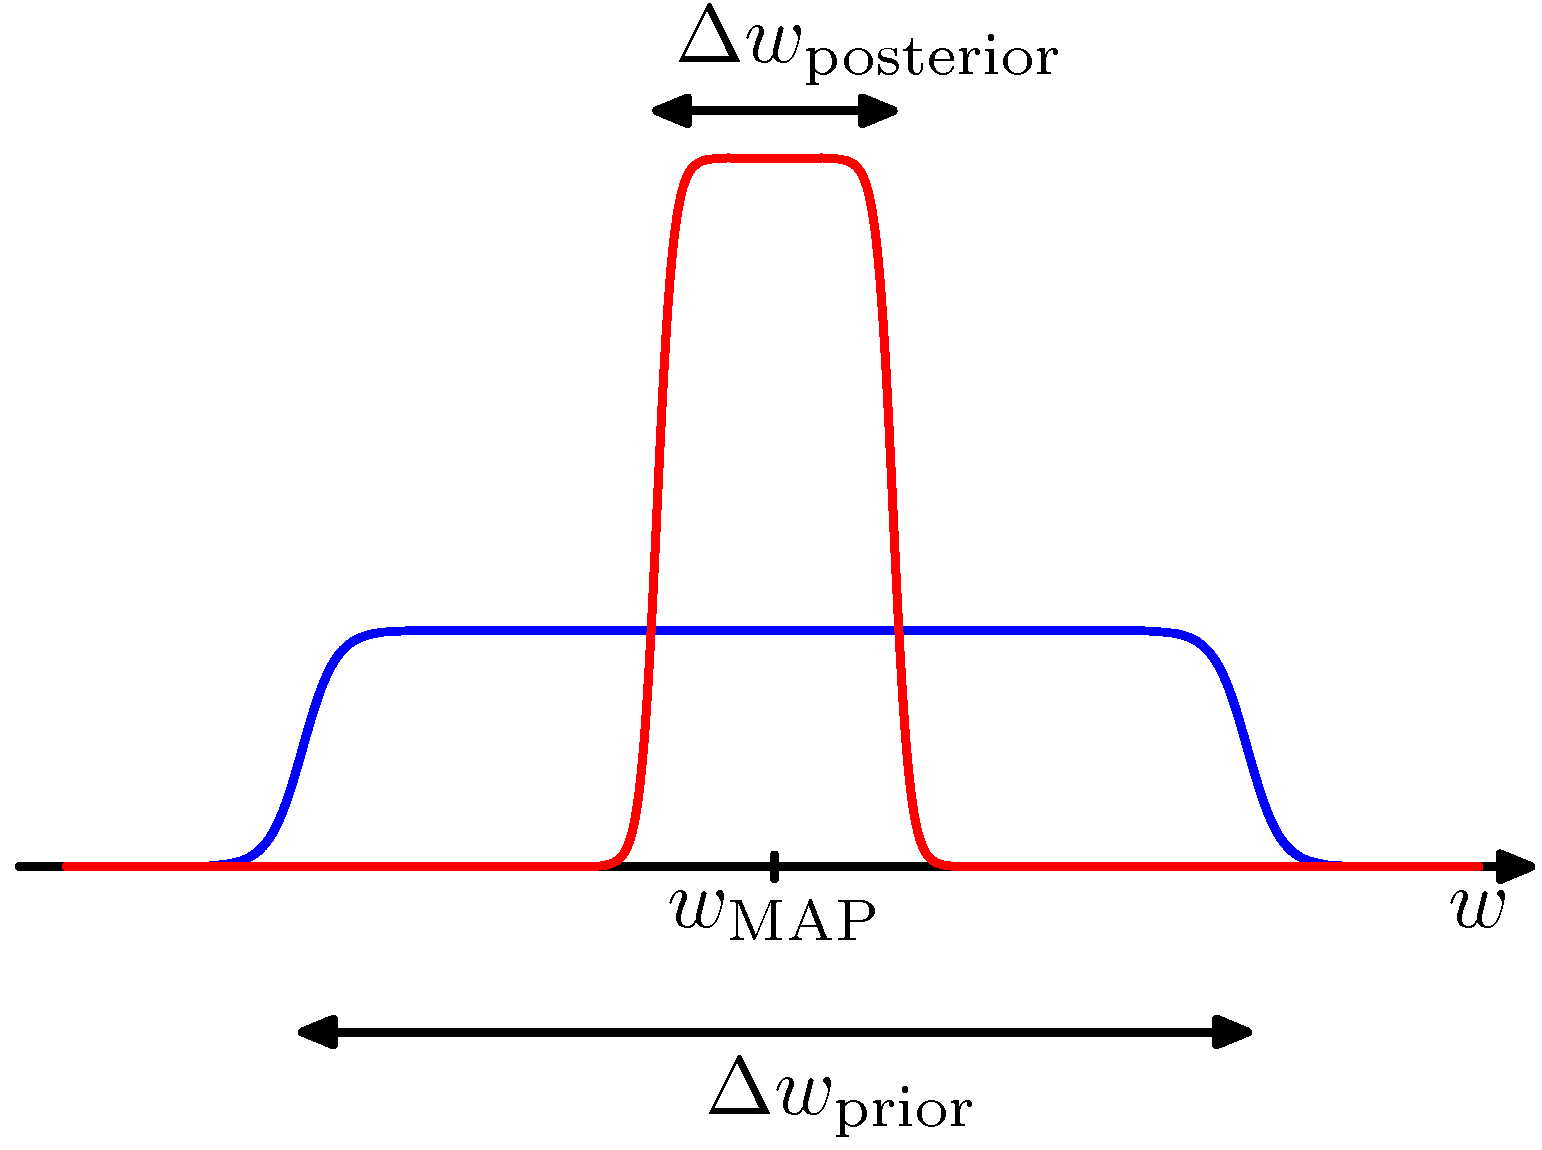
\includegraphics[scale=0.8]{Images/3-12.png}
		\captionsetup{font={small}}
		\caption{如果我们假设参数的后验分布是在其模$w_{\mathrm{MAP}}$附近的尖峰,可以获得如图所示的模型证据粗略近似。}
		\label{fig:3-12}
	\end{figure}
	\\
	\indent 对于带有$M$个参数的模型,可以对每个参数都进行类似的近似。假设所有的参数的$\Delta w_{\mathrm{posterior}} / \Delta w_{\mathrm{prior}}$都相同,可以得到
	\begin{equation}
		\ln p(\calD) \approx \ln p(\calD|\bw_{\mathrm{MAP}})+M\ln \left(\frac{\Delta w_{\mathrm{posterior}}}{\Delta w_{\mathrm{prior}}}\right)
	\end{equation}
	所以在这个非常简单的近似中,复杂度惩罚项会随着模型中可调节参数的数量$M$线性增加。随着我们增加模型的复杂度,第1项通常会增大,因为复杂模型往往能够产生更好的拟合效果,而第2项则会相应减小。最优的模型复杂度是由最大模型证据给出的,而这个复杂度是两个竞争项之间的制衡。随后我们会给出一个更准确的近似,该方法是基于对后验分布进行高斯近似的。\textcolor{red}{\textbf{——第4.4.1节}}\\
	\indent 通过图3.13我们可以进一步理解贝叶斯模型的对比,以及边缘似然是如何促成了中等复杂度的模型。其中,横轴表示的是数据集空间的一维表示,所以横轴上每个点都表示一个数据集。现在我们研究3个模型$\mathcal{M}_1$,$\mathcal{M}_2$和$\mathcal{M}_3$,3个模型的复杂度依次增加。假设现在把3个模型挨个跑了一遍,然后把生成的数据集分布结果拎出来。对于任意的模型都可以生成一系列不同的数据集,因为模型的参数是由先验概率分布控制的,而不管怎样选择参数,目标变量中都会带有随机噪声。为了对某个特定的模型生成某个特定的数据集,首先从参数的先验分布$p(\bw)$中选择参数值,然后对于该参数值,从$p(\calD|\bw)$中抽取数据。类似于一阶多项式这样的简单模型可变性极小,所以生成的数据集区别也不会很大。因此其分布$p(\mathcal{D})$也就被限制在了水平方向上较小的区域中。与之相反,类似于九阶多项式这样的复杂模型生成的数据集变化相当大,所以分布$p(\mathcal{D})$覆盖了横轴相当大的一块区域。由于分布$p(\mathcal{D}|\mathcal{M}_i)$是归一化的,所以某个特定的数据集$\mathcal{D}_0$会在具有中等复杂度的模型上取得最高的模型证据值。从本质上来说,太简单的模型拟合效果肯定不好,太复杂的模型又会造成桃李满天下还必须得雨露均沾的尴尬局面,所以搞得每个数据集都分不到太多的概率。
	\begin{figure}[ht]
		\centering
		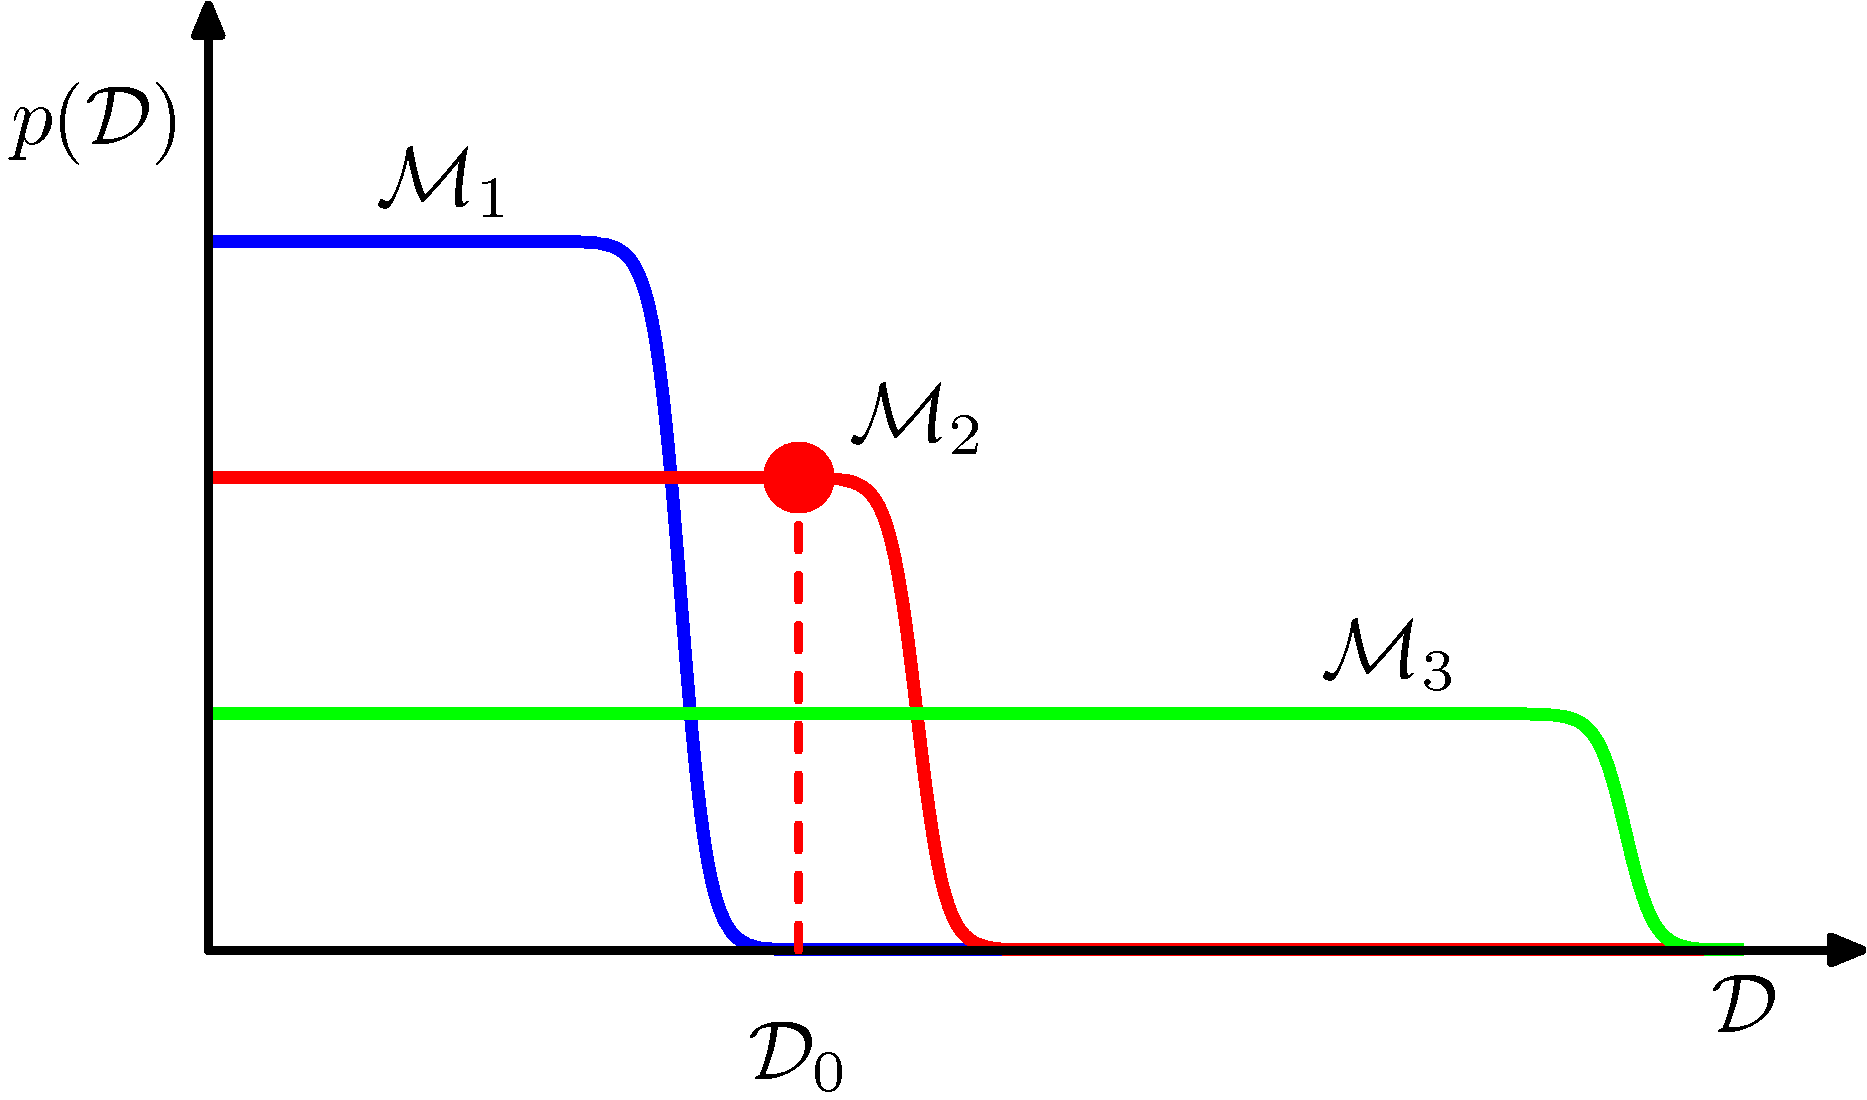
\includegraphics[scale=0.8]{Images/3-13.png}
		\captionsetup{font={small}}
		\caption{三种不同复杂度的模型各自的数据集分布,$\mathcal{M}_1$是复杂度最低的,$\mathcal{M}_3$的复杂度最高的。这些分布都是经过归一化的。在这个例子中,对于某个数据集$\calD_0$,中等复杂的模型$\mathcal{M}_2$给出的模型证据最大。}
		\label{fig:3-13}
	\end{figure}
	\\
	\indent 贝叶斯模型的比较中隐含了一个假设,那就是真实的分布(数据的真实来源)存在于模型集合中。如果事实如此,我们可以证明贝叶斯模型的对比是倾向于正确模型的。为了证明这个问题,假设有两个模型$\mathcal{M}_1$和$\mathcal{M}_2$,正确的模型是$\mathcal{M}_1$。对于一个给定的有限数据集,错误的模型会产生较大的贝叶斯因子。然而,如果我们在整个数据集分布上对贝叶斯因子求平均数,就可以得到期望贝叶斯因子:
	\begin{equation}
		\int p(\mathcal{D}|\mathcal{M}_1)\ln \frac{p(\calD|\mathcal{M}_1)}{p(\calD|\mathcal{M}_2)}\ \mathrm{d}\mathcal{D}
	\end{equation}
	其中已经关于数据的真实分布求取了平均值。这个值是KL距离的典型案例,\textcolor{red}{\textbf{——第1.6.1节}}\ 它满足一条性质,即只要两个分布不相等,这个距离就一定为正,当且仅当两个分布完全相同时,这个距离为0。所以一般情况下,贝叶斯因子始终倾向于正确的模型。\\
	\indent 我们已经可以看出,贝叶斯学习可以避免过拟合的问题,而且仅基于训练数据就可以进行模型之间的对比。然而,和其他的模式识别方法一样,贝叶斯方法也需要对模型的形式做出假设。如果这些假设是不合理的,那么结果也会非常糟糕。特别地,从图3.12可以看出,模型证据对先验的诸多方面都很是神经过敏,尤其是拖尾的部分。实际上,如果先验是反常的,那么模型证据就是无意义的。一个反常的先验可以有任意的缩放因子,换句话说,这个分布压根就不可能被归一化,所以归一化参数是没意义的,所以模型证据也是无意义的。如果对一个适当的先验取适当的极限,这样得到的反常先验(比如高斯先验带上一个无限大的方差这样的反常先验)会使得模型证据趋向于0,这点可以从(3.70)和图3.12看出来。不过即使是这种情况,也可以首先求取两个模型的模型证据比值,然后取极限,从而得到一个可用的结果。\\
	\indent 所以在实际应用中,首先保留一个独立的测试数据集是比较明智的,因为这样可以评估最终得到的系统的整体表现。
	}
	\section{证据近似}
	\insertline\\
	\textnormal{
	\indent 在完整的贝叶斯方法下的线性基底函数模型中,我们会引入关于超参数$\alpha$和$\beta$的先验分布,并对这些超参数以及参数$\bw$进行边缘化,从而进行预测。然而,尽管在理论上我们可以对$\bw$和超参数们进行边缘化,但对这些参数进行彻底边缘化的计算代价是相当大的。现在我们要研究是一种近似方法,在这个方法中,我们通过对边缘似然函数(marginal likelihood function)进行最小化,将超参数设定为特定的值。这里的边缘似然函数是首先对参数$\bw$积分得到的。这个办法在统计学领域称为经验贝叶斯方法(empirical Bayes, Bernardo and Smith, 1994; Gelman et al., 2004)或者第二型最大似然方法(type 2 maximum likelihood, Berger, 1985),亦或称为广义最大似然方法(generalized maximum likelihood, Wahba, 1975),不过在机器学习领域,一般称为证据近似(evidence approximation, Gull, 1989; MacKay, 1992a)。\\
	\indent 假设现在引入$\alpha$和$\beta$的超先验,那么对$\bw$,$\alpha$和$\beta$进行边缘化即可得到预测分布
	\begin{equation}
		p(t|\sft) = \iiint p(t|\bw, \beta)p(\bw|\sft,\alpha,\beta)p(\alpha, \beta|\sft)\ \rmd \bw \ \rmd \alpha \ \rmd \beta
	\end{equation}
	其中$p(t|\bw, \beta)$为(3.8)所定义的,$p(\bw|\sft, \alpha, \beta)$为(3.49)所定义的,其中的$\mathbf{m}_N$和$\mathbf{S}_N$为(3.53)和(3.54)所定义的。为了简化符号,现在开始省略依赖项中的输入变量$\bx$。如果后验分布$p(\alpha,\beta|\sft)$是$\hat{\alpha}$和$\hat{\beta}$附近的尖峰,那么就可以将$\alpha$和$\beta$设定为固定的$\hat{\alpha}$和$\hat{\beta}$,于是只对$\bw$进行边缘化就可以得到预测分布:
	\begin{equation}
		p(t|\sft) \approx p(t|\sft, \hat{\alpha}, \hat{\beta}) = \int p(t|\bw, \hat{\beta})p(\bw|\sft, \hat{\alpha}, \hat{\beta})\ \rmd \bw
	\end{equation}
	根据贝叶斯定理,$\alpha$和$\beta$的后验分布为
	\begin{equation}
		p(\alpha, \beta|\sft) \propto p(\sft|\alpha , \beta)p(\alpha , \beta)
	\end{equation}
	如果先验比较平坦,那么在模型证据中,可以通过对边缘似然函数$p(\sft|\alpha,\beta)$进行最大化来获得$\hat{\alpha}$和$\hat{\beta}$。接下来我们会评估线性基底函数模型的边缘似然函数,并求其最大值。这样的做法使得我们仅通过训练数据就可以确定超参数的值,而不需要交叉验证这样的步骤。回想一下,比值$\alpha/\beta$是类似于正则化参数的。\\
	\indent 此外还有一点值得注意,如果我们定义了$\alpha$和$\beta$的共轭先验分布(Gamma先验分布),那么对于这些超参数根据(3.74)进行边缘化,得到的结果事实上就是一个关于$\bw$的学生t分布,相关的内容详见第2.3.7节。尽管关于$\bw$的积分不再有解析形式,但对这个积分求近似也会给出模型证据的替代结果(Buntine and Weigend, 1991),比如即将在第4.4节中讨论的Laplace近似。Laplace近似是基于局部高斯近似的近似方法,这里的局部高斯近似是以后验概率分布的模为中心的近似。然而,被积函数是$\bw$的函数,而它的模往往不太准确,所以Laplace近似往往无法准确描述概率质量函数中的信息,这可能导致最终的结果比证据最大化方法得到的结果还差(MacKay, 1999)。\\
	\indent 回到模型证据的讨论中来,我们注意到有两种将对数模型证据进行最大化的方法。一方面,我们可以解析地评估证据函数并令其导数为0,从而得到新的$\alpha$和$\beta$的估计结果,这个方法我们将在第3.5.2节中进行讨论;另一方面,我们可以利用即将在第9.3.4节中讨论的EM算法,到时候我们还会证明这两种方法事实上会收敛到同一个解。
	}
	\subsection{证据函数的评估}
	\textnormal{
	边缘似然函数$p(\sft|\alpha,\beta)$是通过对权重参数$\bw$进行边缘化得到的,于是
	\begin{equation}
		p(\sft|\alpha,\beta)=\int p(\sft|\bw, \beta)p(\bw|\alpha)\ \rmd \bw
	\end{equation}
	评估这个积分,一种方法是再次利用线性高斯模型的条件分布的结论(2.115)。\textcolor{red}{\textbf{——习题3.16}}\ 现在我们通过对指数项进行完成平方项,并利用高斯函数的归一化系数的标准形式,评估这个积分。\\
	\indent 根据(3.11),(3.12)和(3.52),可以将证据函数写成如下形式:\textcolor{red}{\textbf{——习题3.17}}
	\begin{equation}
		p(\sft|\alpha,\beta) = \left(\frac{\beta}{2\pi}\right)^{N/2} \left(\frac{\alpha}{2\pi}\right)^{M/2} \int \exp\{-E(\bw)\}\ \rmd \bw
	\end{equation}
	其中$M$为向量$\bw$的维度,以及
	\begin{equation}
	\begin{split}
		E(\bw) &= \beta E_D(\bw) + \alpha E_W(\bw) \\
		&= \frac{\beta}{2}\|\sft - \bfPhi \bw \|^2 + \frac{\alpha}{2}\bw^{\rmT} \bw
	\end{split}
	\end{equation}
	可以看出(3.79)修改一下系数就与正则化平方和误差函数(3.27)是相等了。\textcolor{red}{\textbf{——习题3.18}}\ 现在关于$\bw$进行完成平方项,
	\begin{equation}
		E(\bw) = E(\mathbf{m}_N) + \frac{1}{2}(\bw - \mathbf{m}_N)^{\rmT} \mathbf{A} (\bw - \mathbf{m}_N)
	\end{equation}
	其中
	\begin{equation}
		\mathbf{A}=\alpha \mathbf{I} + \beta \bfPhi^{\rmT} \bfPhi
	\end{equation}
	以及
	\begin{equation}
		E(\mathbf{m}_N) = \frac{\beta}{2}\|\sft - \bfPhi\mathbf{m}_N\|^2 + \frac{\alpha}{2}\mathbf{m}_N^{\rmT}\mathbf{m}_N
	\end{equation}
	需要注意的是,$\mathbf{A}$是误差函数的二阶导数
	\begin{equation}
		\mathbf{A}=\nabla \nabla E(\bw)
	\end{equation}
	也就是海森矩阵(Hessian matrix)。同时还可以定义$\mathbf{m}_N$
	\begin{equation}
		\mathbf{m}_N = \beta \mathbf{A}^{-1}\bfPhi^{\rmT} \sft
	\end{equation}
	根据(3.54),我们可以看出$\mathbf{A} = \mathbf{S}_N^{-1}$,所以(3.84)是等价于(3.53)的,表示后验分布的均值。\\
	\indent 现在可以通过与多元高斯分布归一化系数的标准结果做一下对比,从而评估这个关于$\bw$的积分,即\textcolor{red}{\textbf{——习题3.19}}
	\begin{equation}
	\begin{split}
		&\int \exp\{-E(\bw)\}\ \rmd \bw \\
		= &\exp\{-E(\mathbf{m}_N)\}\int \exp\left\{-\frac{1}{2}(\bw - \mathbf{m}_N)^{\rmT}\mathbf{A}(\bw - \mathbf{m}_N)\right\}\ \rmd \bw \\
		= &\exp\{-E(\mathbf{m}_N)\}(2\pi)^{M/2}|\mathbf{A}|^{-1/2}
	\end{split}
	\end{equation}
	根据(3.78),可以写出对数边缘似然函数
	\begin{equation}
		\ln p(\sft|\alpha,\beta) =\frac{M}{2}\ln \alpha + \frac{N}{2} \ln \beta - E(\mathbf{m}_N) -\frac{1}{2}\ln |\mathbf{A}| - \frac{N}{2}\ln (2\pi)
	\end{equation}
	这就是我们所需要的证据函数的表达式。\\
	\indent 回到多项式回归问题中,我们可以关于多项式的阶数画出模型证据的图像,如图3.14所示。这里我们假设先验为(1.65)这样的形式,且参数$\alpha = 5 \times 10^{-1}$。这个图像非常有指导意义。回看一下图1.4,可以看出$M=0$的多项式对数据的拟合效果相当差,所以其模型证据也很低。当$M=1$时,拟合的效果好了很多,模型证据也高了很多。不过,当$M=2$时,拟合效果又变差了,因为真实的函数是正弦函数,而正弦函数的展开项里是没有偶数项的幂函数的。图1.5也展示了$M=1$变化成$M=2$时,数据残差仅有微小的减小,而且由于复杂模型的复杂度惩罚项很大,所以在这个过程中,模型证据减小了。当$M=3$时,模型对数据的拟合效果得到了大幅的提升,所以模型证据也再次提升了,而且达到了所有多项式拟合中的最大值。在此之后,即使再次增加$M$的值,拟合的效果也只能得到稍许的提升,而模型复杂度却上升了,所以惩罚项也会随之变大,导致模型证据的下降。再看一下图1.5,在$M=3$到$M=8$之间,泛化误差几乎就是一个常数,所以很难据此选择模型。不过,模型证据的结果很明显更加青睐$M=3$的模型,因为这是能够较准确描述数据的最简单的模型。
	\begin{figure}[ht]
		\centering
		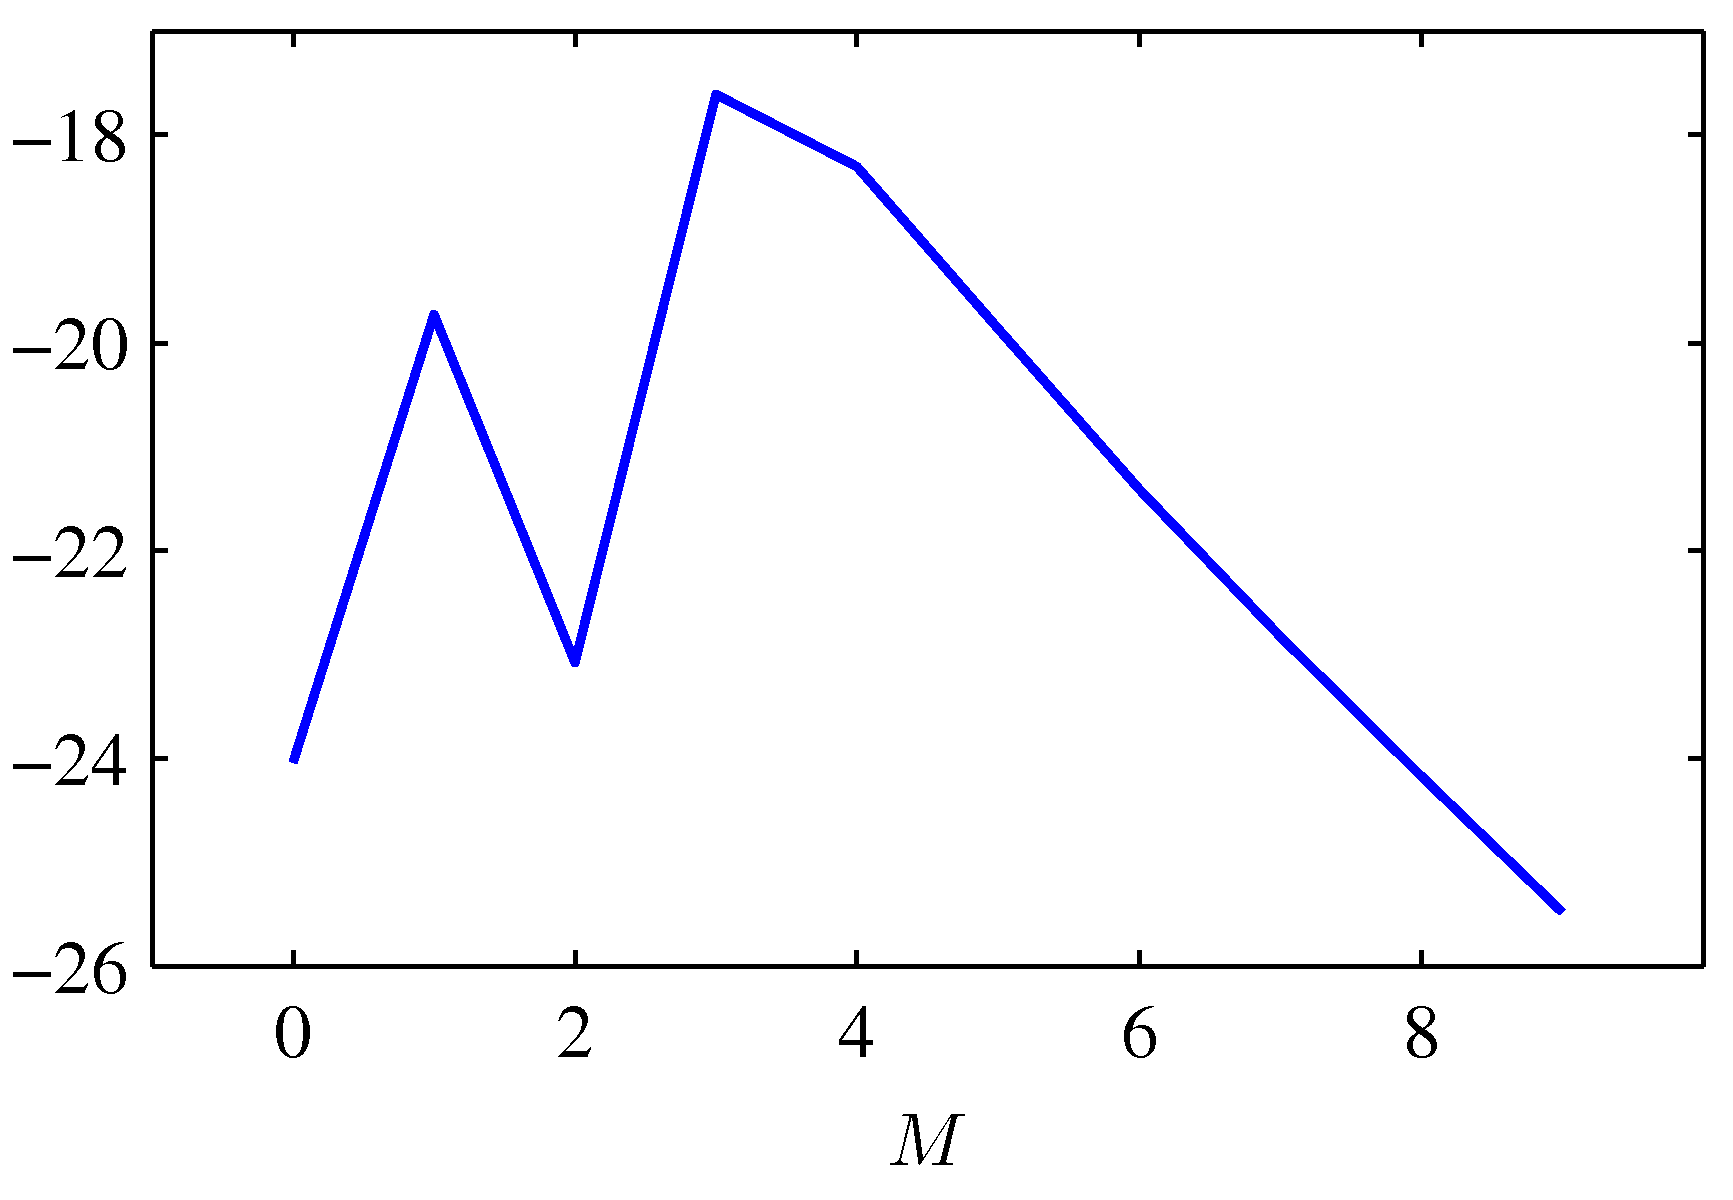
\includegraphics[scale=0.8]{Images/3-14.png}
		\captionsetup{font={small}}
		\caption{关于阶数$M$绘制的模型对数证据的图像,对于多项式回归模型而言,模型证据最倾向于选择$M=3$的模型。}
		\label{fig:3-14}
	\end{figure}
	}
	\subsection{证据函数的最大化}
	\textnormal{
	首先研究$p(\sft|\alpha,\beta)$关于$\alpha$的最大化。首先定义特征向量等式
	\begin{equation}
		(\beta \bfPhi^{\rmT}\bfPhi)\mathbf{u}_i = \lambda_i \mathbf{u}_i
	\end{equation}
	根据(3.81),$\mathbf{A}$的特征值为$\alpha + \lambda_i$。现在对(3.86)中含有$\ln |\mathbf{A}|$的项关于$\alpha$求导数,可得
	\begin{equation}
		\frac{d}{d\alpha}\ln |\mathbf{A}| = \frac{d}{d\alpha}\ln \prod_{i}(\lambda_i + \alpha) = \frac{d}{d\alpha}\sum_{i} \ln (\lambda_i+\alpha)=\sum_{i}\frac{1}{\lambda_i+\alpha}
	\end{equation}
	于是(3.86)关于$\alpha$的驻点满足
	\begin{equation}
		0 = \frac{M}{2\alpha} - \frac{1}{2}\mathbf{m}_N^{\rmT}\mathbf{m}_N - \frac{1}{2}\sum_{i}\frac{1}{\lambda_i + \alpha}
	\end{equation}
	两侧同时乘以$2\alpha$并重新组织一下,
	\begin{equation}
		\alpha \mathbf{m}_N^{\rmT} \mathbf{m}_N = M - \alpha \sum_{i}\frac{1}{\lambda_i \alpha} = \gamma
	\end{equation}
	由于求和项中共有$M$项,于是$\gamma$可以写成
	\begin{equation}
		\gamma = \sum_{i}\frac{\lambda_i}{\alpha + \lambda_i}
	\end{equation}
	简单解释一下$\gamma$的含义。根据(3.90)可以看出使得边缘似然函数取得最大值的$\alpha$满足\textcolor{red}{\textbf{——习题3.20}}
	\begin{equation}
		\alpha = \frac{\gamma}{\mathbf{m}_N^{\rmT}\mathbf{m}_N}
	\end{equation}
	这是一个$\alpha$的隐式解,一方面是因为$\gamma$与$\alpha$是相关的,另一方面也是因为后验分布的模$\mathbf{m}_N$本身也依赖于$\alpha$。所以我们采用迭代的方式来求解这个方程。首先选取一个$\alpha$的初始值,然后用它根据(3.53)去求$\mathbf{m}_N$,根据(3.91)计算$\gamma$。接下来利用这些结果根据(3.92)重新估计$\alpha$,直到收敛为止。由于矩阵$\bfPhi^{\rmT}\bfPhi$是固定的,我们可以在开始阶段计算它的特征值,然后在每一步更新中乘以$\beta$就可以得到$\lambda_i$了。\\
	\indent 有个需要强调一下的地方,那就是$\alpha$的值是完全通过对训练集的观察得到的。与最大似然方法需要独立的数据集来优化模型复杂度不同,这里不需要这样的措施。\\
	\indent 类似地,我们也可以将对数边缘似然函数(3.86)关于$\beta$进行最大化。为了做到这一点,首先注意到(3.87)中的特征值$\lambda_i$与$\beta$成正比,所以$d\lambda_i/d\beta = \lambda_i/\beta$,于是
	\begin{equation}
		\frac{d}{d\beta} \ln |\mathbf{A}| = \frac{d}{d\beta}\sum_{i} \ln (\lambda_i + \alpha)=\frac{1}{\beta}\sum_{i}\frac{\lambda_i}{\lambda_i+\alpha}=\frac{\gamma}{\beta}
	\end{equation}
	于是边缘似然函数的驻点满足条件
	\begin{equation}
		0 = \frac{N}{2\beta} - \frac{1}{2}\sum_{n=1}^N \left\{t_n-\mathbf{m}_N^{\rmT}\bfphi(\bx_n)\right\}^2 - \frac{\gamma}{2\beta}
	\end{equation}
	重新整理一下,\textcolor{red}{\textbf{——习题3.22}}
	\begin{equation}
		\frac{1}{\beta}=\frac{1}{N-\gamma}\sum_{n=1}^N \left\{t_n - \mathbf{m}_N^{\rmT}\bfphi(\bx_n)\right\}^2
	\end{equation}
	和以前一样,这又是一个关于$\beta$的隐式解,可以首先选取$\beta$的初始值,然后计算$\mathbf{m}_N$和$\gamma$,再利用(3.95)更新$\beta$,直到收敛为止。如果$\alpha$和$\beta$的值要根据数据确定,那么可以在$\gamma$更新之后一起重新估计。
	}
	\subsection{有效参数的数量}
	\textnormal{
	其实(3.92)还有另一种很不错的诠释(MacKay, 1992a),可以对$\alpha$进行更加深刻的贝叶斯解释。为了看出这一点,我们研究一下如图3.15所示的似然函数与先验的轮廓线。这里我们比较隐晦地对参数空间的坐标轴进行了旋转变换,从而与(3.87)所定义的特征向量对齐。于是似然函数的轮廓线椭圆的两轴也与坐标轴对齐了。特征值$\lambda_i$衡量的是似然函数的曲率,所以在图3.15中,特征值$\lambda_1$比$\lambda_2$要小(因为曲率越小,似然函数的轮廓线就越扁)。由于$\beta \bfPhi^{\rmT} \bfPhi$是正定矩阵,所以其特征值均为正数,所以比值$\lambda_i / (\lambda_i+\alpha)$是处于0和1之间的数。再多推进一步,(3.91)中的$\gamma$一定是位于范围$0 \leqslant \gamma \leqslant M$中的。对于$\lambda_i \gg \alpha$的方向,对应的参数$w_i$将非常接近其最大似然值,比值$\lambda_i / (\lambda_i+\alpha)$也将非常接近1.这样的参数被称为well determined参数,因为它们的值严格受到数据的控制。相反,对于$\lambda_i \ll \alpha$的方向,对应的参数$w_i$接近于0,所以$\lambda_i / (\lambda_i+\alpha)$也会随之非常接近0。在这样的方向上,似然函数对参数值非常不敏感,所以先验会将参数设置为较小的值。所以(3.91)中的$\gamma$衡量的其实是well determined参数中有效参数的数量。
	\begin{figure}[ht]
		\centering
		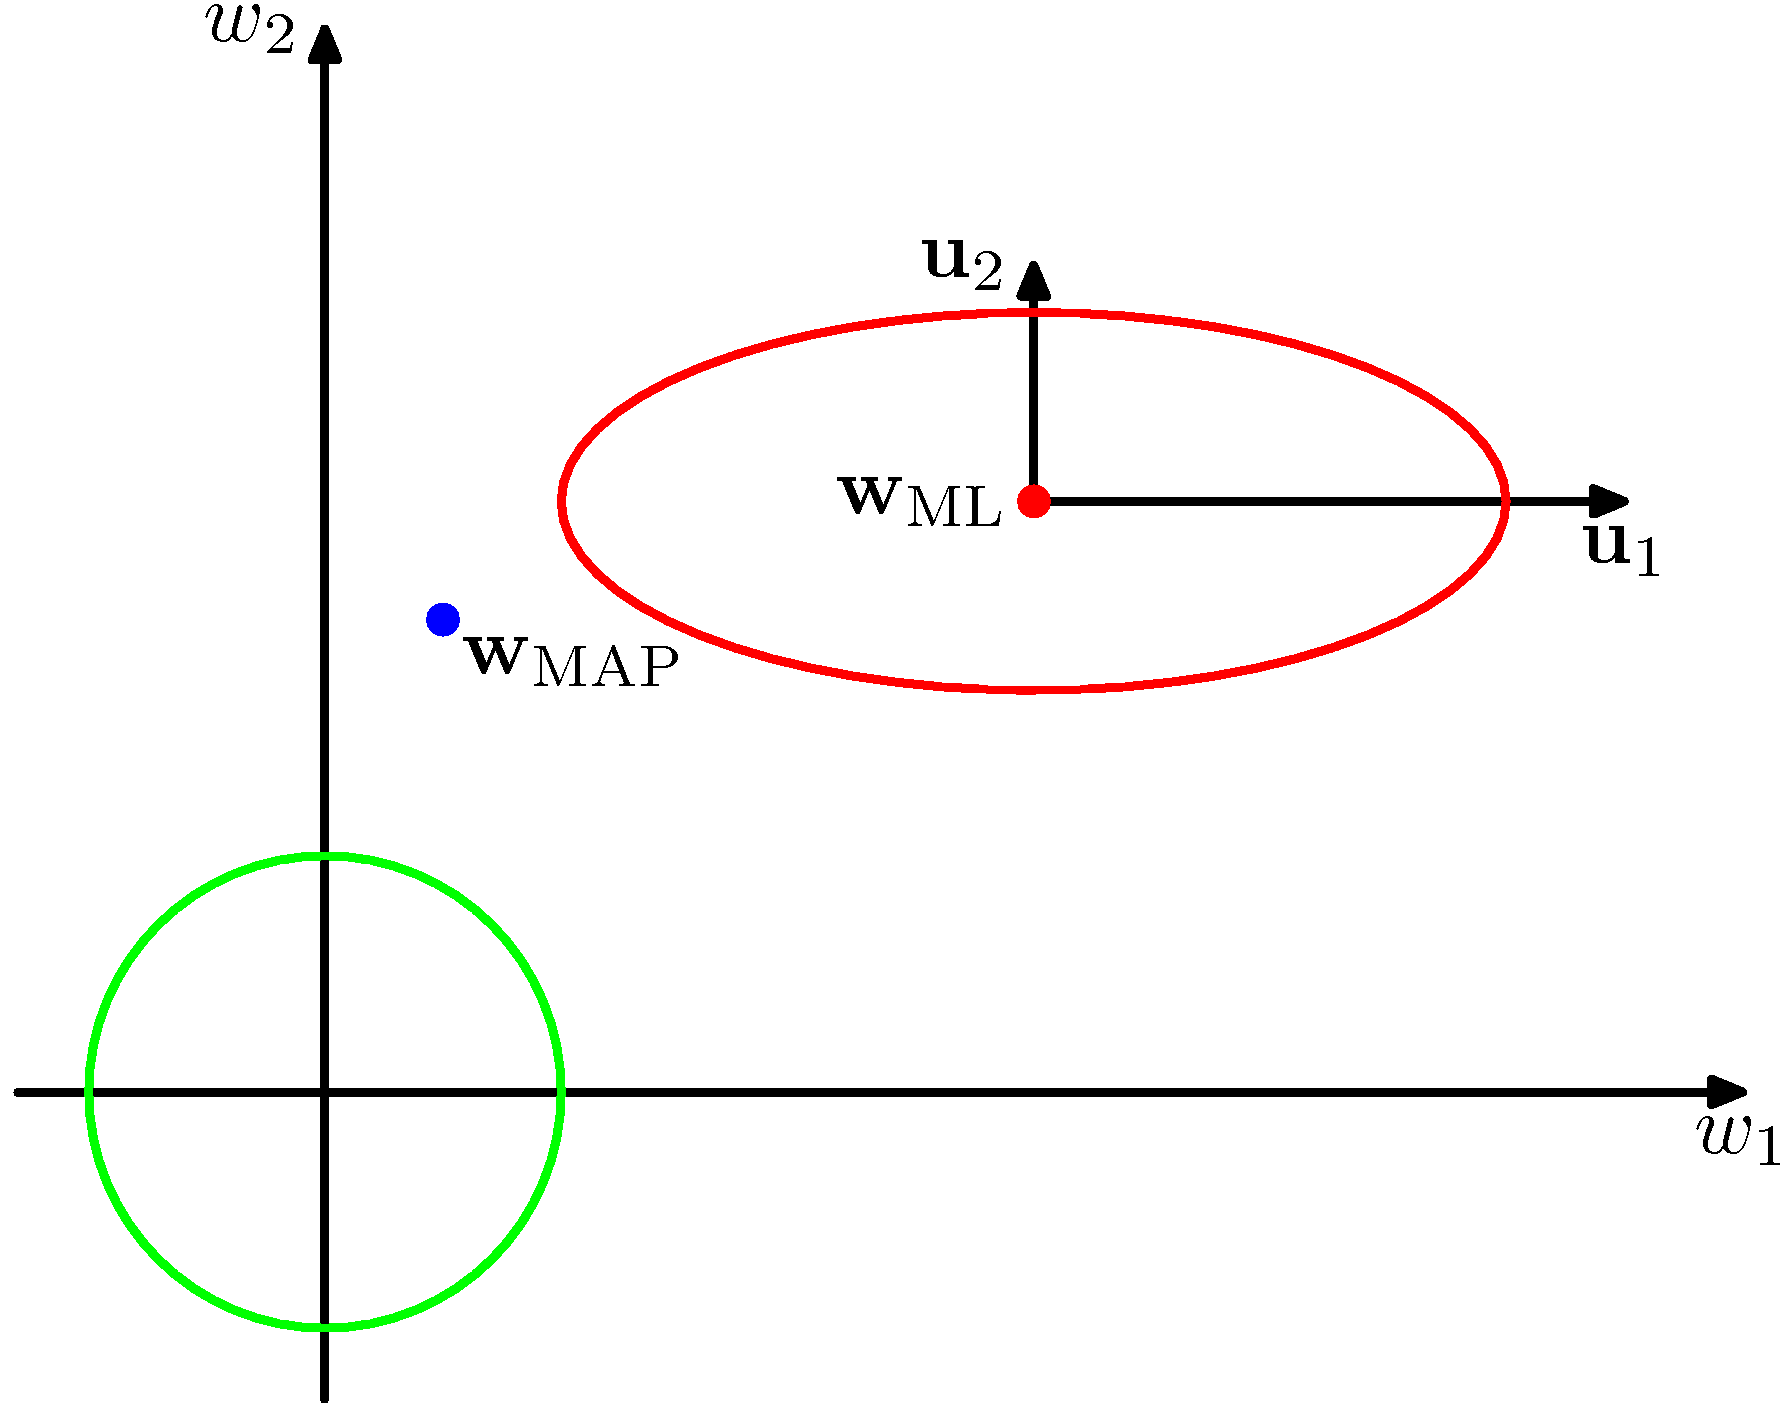
\includegraphics[scale=0.9]{Images/3-15.png}
		\captionsetup{font={small}}
		\caption{似然函数的轮廓线(红色曲线)和先验概率分布(绿色曲线),参数空间的坐标轴经过旋转后与Hessian矩阵的特征向量$\mathbf{u}_i$对齐。对于$\alpha=0$,后验的模为最大似然解$\bw_{\mathrm{ML}}$,而对于$\alpha \ne 0$,模则位于$\bw_{\mathrm{MAP}}=\mathbf{m}_N$。在方向$w_1$上,由(3.87)定义的特征值$\lambda$比$\alpha$小,因此$\lambda_1 / (\lambda_1+\alpha)$接近于0,于是$w_1$的MAP值也接近于0。与之相反,在$w_2$的方向上,特征值$\lambda_2$大于$\alpha$,因此 $\lambda_2 / (\lambda_2+\alpha)$接近于1,$w_2$的MAP值接近于最大似然值。}
		\label{fig:3-15}
	\end{figure}
	\\
	\indent 我们可以通过将重新估计$\beta$的(3.95)与对应的最大似然解(3.21)做一下对比,从而得出更深刻的理解。这两个公式都将方差(精度的逆)表示为目标与模型预测之间误差求平方后再求平均得到的值。它们的区别在于,最大似然解的分母中数据点的数量是$N$,贝叶斯方法中则是$N-\gamma$。回想一下(1.56),一元高斯分布方差的最大似然估计为
	\begin{equation}
		\sigma_{\mathrm{ML}}^2 = \frac{1}{N}\sum_{n=1}^N (x_n - \mu_{\mathrm{ML}})^2
	\end{equation}
	而且这个估计是有偏估计,因为期望的最大似然解$\mu_{\mathrm{ML}}$中包含了数据中的噪声。于是这会占用模型中的一个自由度。对应的无偏估计是(1.59),形式为
	\begin{equation}
		\sigma_{\mathrm{MAP}}^2 = \frac{1}{N-1}\sum_{n=1}^N (x_n - \mu_{\mathrm{ML}})^2
	\end{equation}
	贝叶斯方法给出的解中,分母中的因子$N-1$反映了一个自由度被均值占用了的这件事情,并相应修正了最大似然的偏差。现在研究一下线性回归模型中的相应结果,目标分布的均值为$\bw^{\rmT}\bfphi(\bx)$,其中包含$M$个参数。不过并非所有的参数都是适合数据的。其中根据数据确定的有效参数数量为$\gamma$,而且先验将其余的$M-\gamma$个参数设置为较小的值。在贝叶斯方法给出的结果中也有所反映,即分母中的因子$N-\gamma$,修正了最大似然解中的偏差。\\
	\indent 我们可以在第1.1节中的正弦函数数据集中使用包含9个基底函数的高斯基底函数模型的模型证据来设定超参数,所以模型中的参数总数为$M=10$,其中包含了偏差。为了简化起见,现在将$\beta$设定为真实值11.1,然后使用模型证据确定$\alpha$,如图3.16所示。
	\begin{figure}[ht]
		\begin{minipage}[t]{0.5\linewidth}
		\centering
		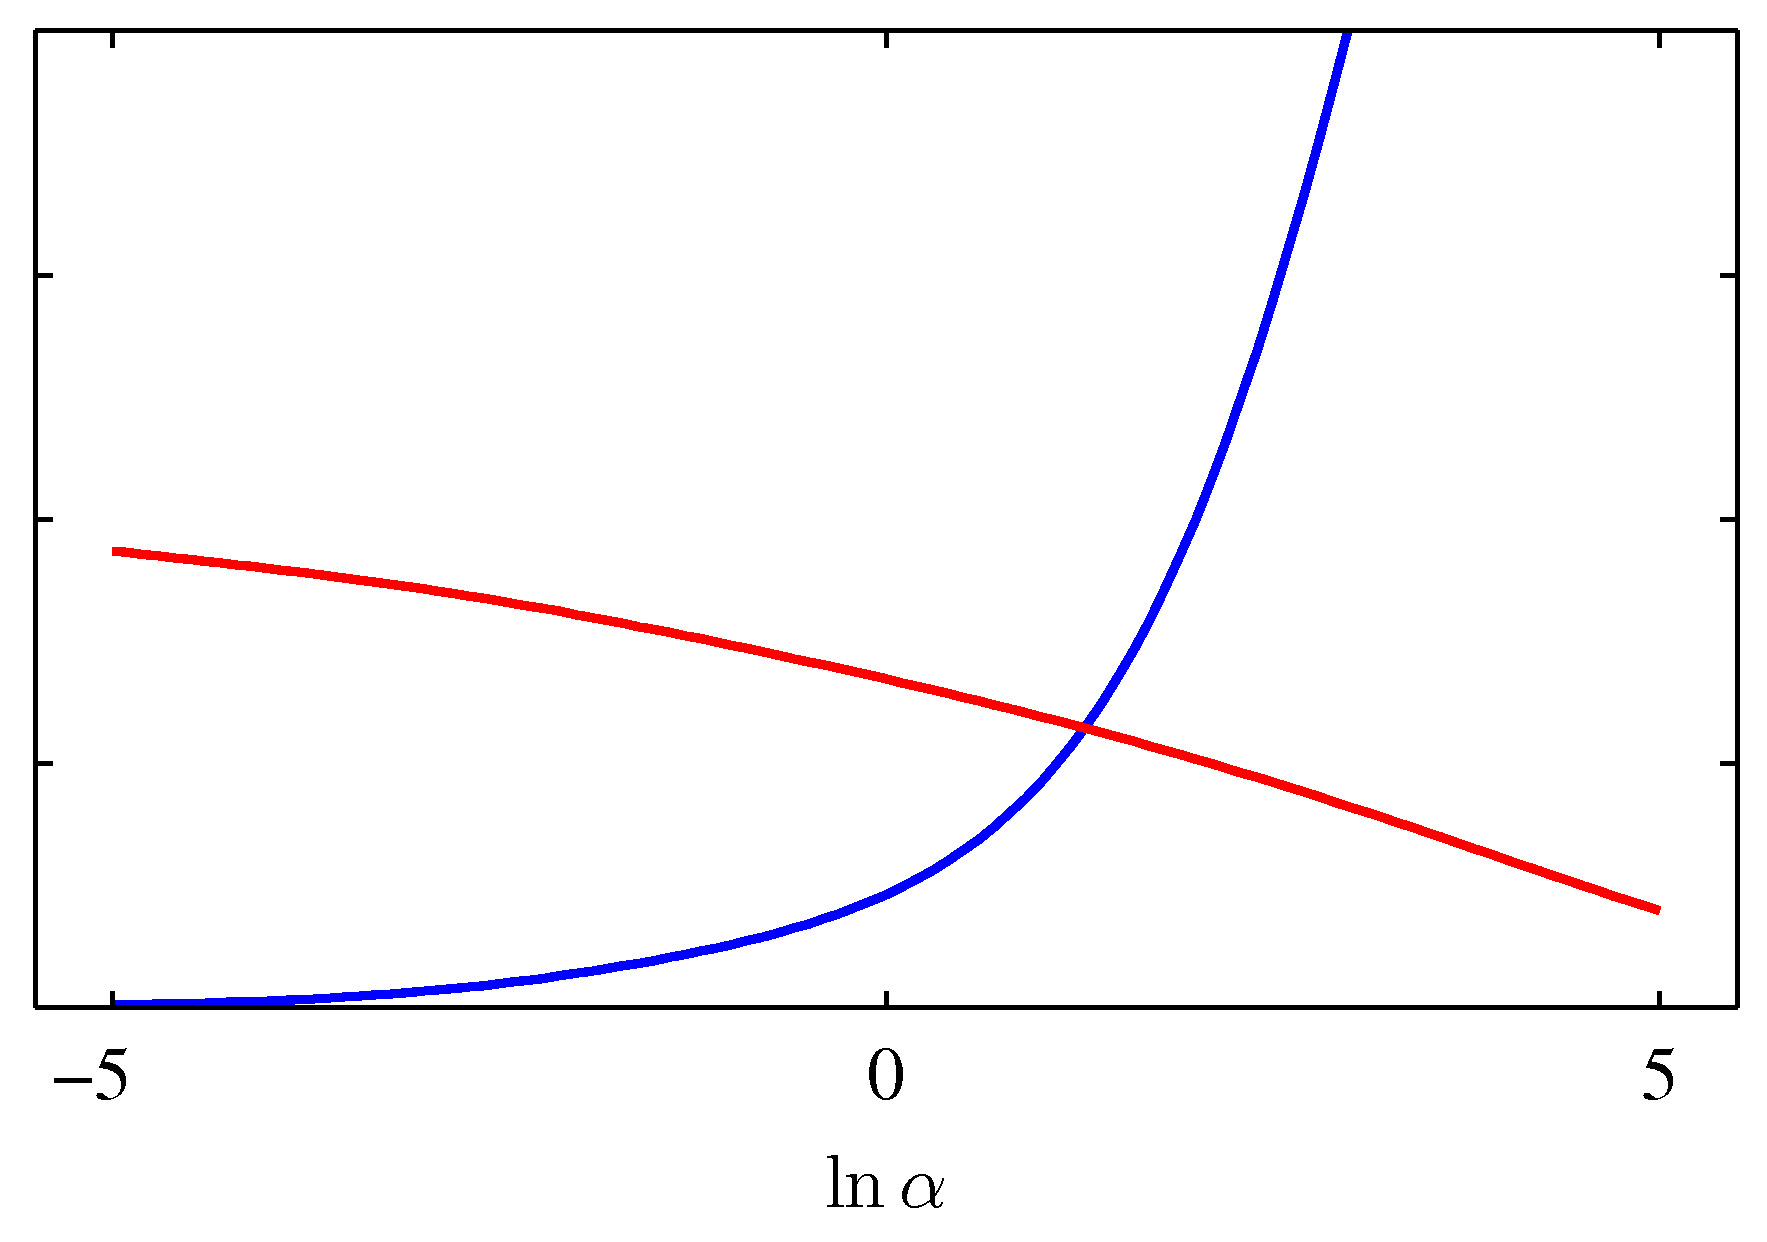
\includegraphics[scale=0.8]{Images/3-16a.png}
		\label{fig:3-16a}
		\end{minipage}
		\begin{minipage}[t]{0.5\linewidth}
		\centering
		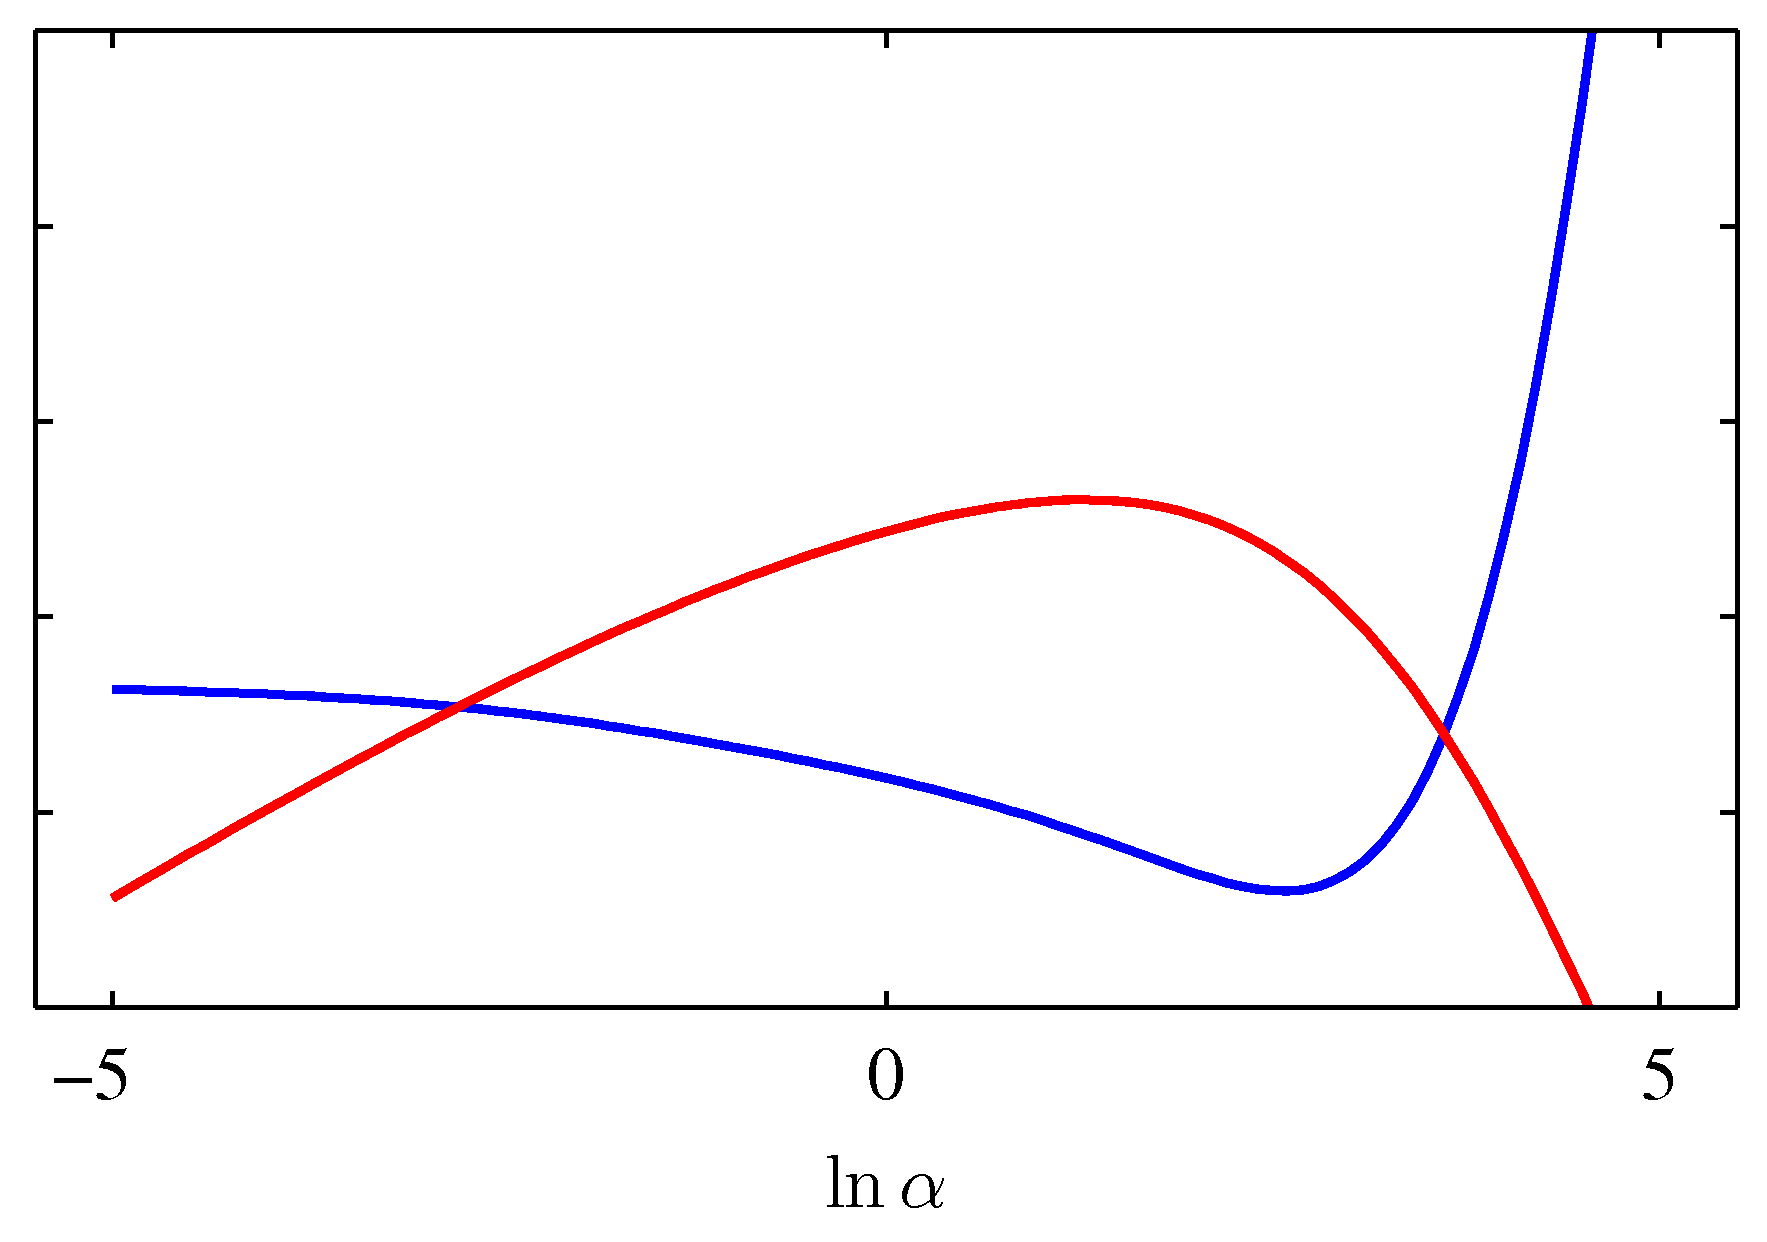
\includegraphics[scale=0.8]{Images/3-16b.png}
		\label{fig:3-16b}
		\end{minipage}
		\captionsetup{font={small}}
		\caption{左图为$\gamma$和$2\alpha E_W(\mathbf{m}_N)$与$\ln \alpha$的函数关系(分别为红色曲线和蓝色曲线),这里的数据集是正弦函数数据集。这两条曲线的交点正是最优解$\alpha$。右图中的红色曲线是对数模型证据$\ln p(\sft|\alpha,\beta)$关于$\ln \alpha$的函数关系,恰好在左图中的交点处取得峰值。蓝色曲线为测试集误差,验证了在模型证据取得最大值时模型具有最优的泛化能力。}
	\end{figure}
	\\
	\indent 我们还可以通过绘制出独立参数与有效参数数量$\gamma$之间函数关系的的图像(如图3.17所示),看出参数$\alpha$控制着参数$\{w_i\}$。
	\begin{figure}[ht]
		\centering
		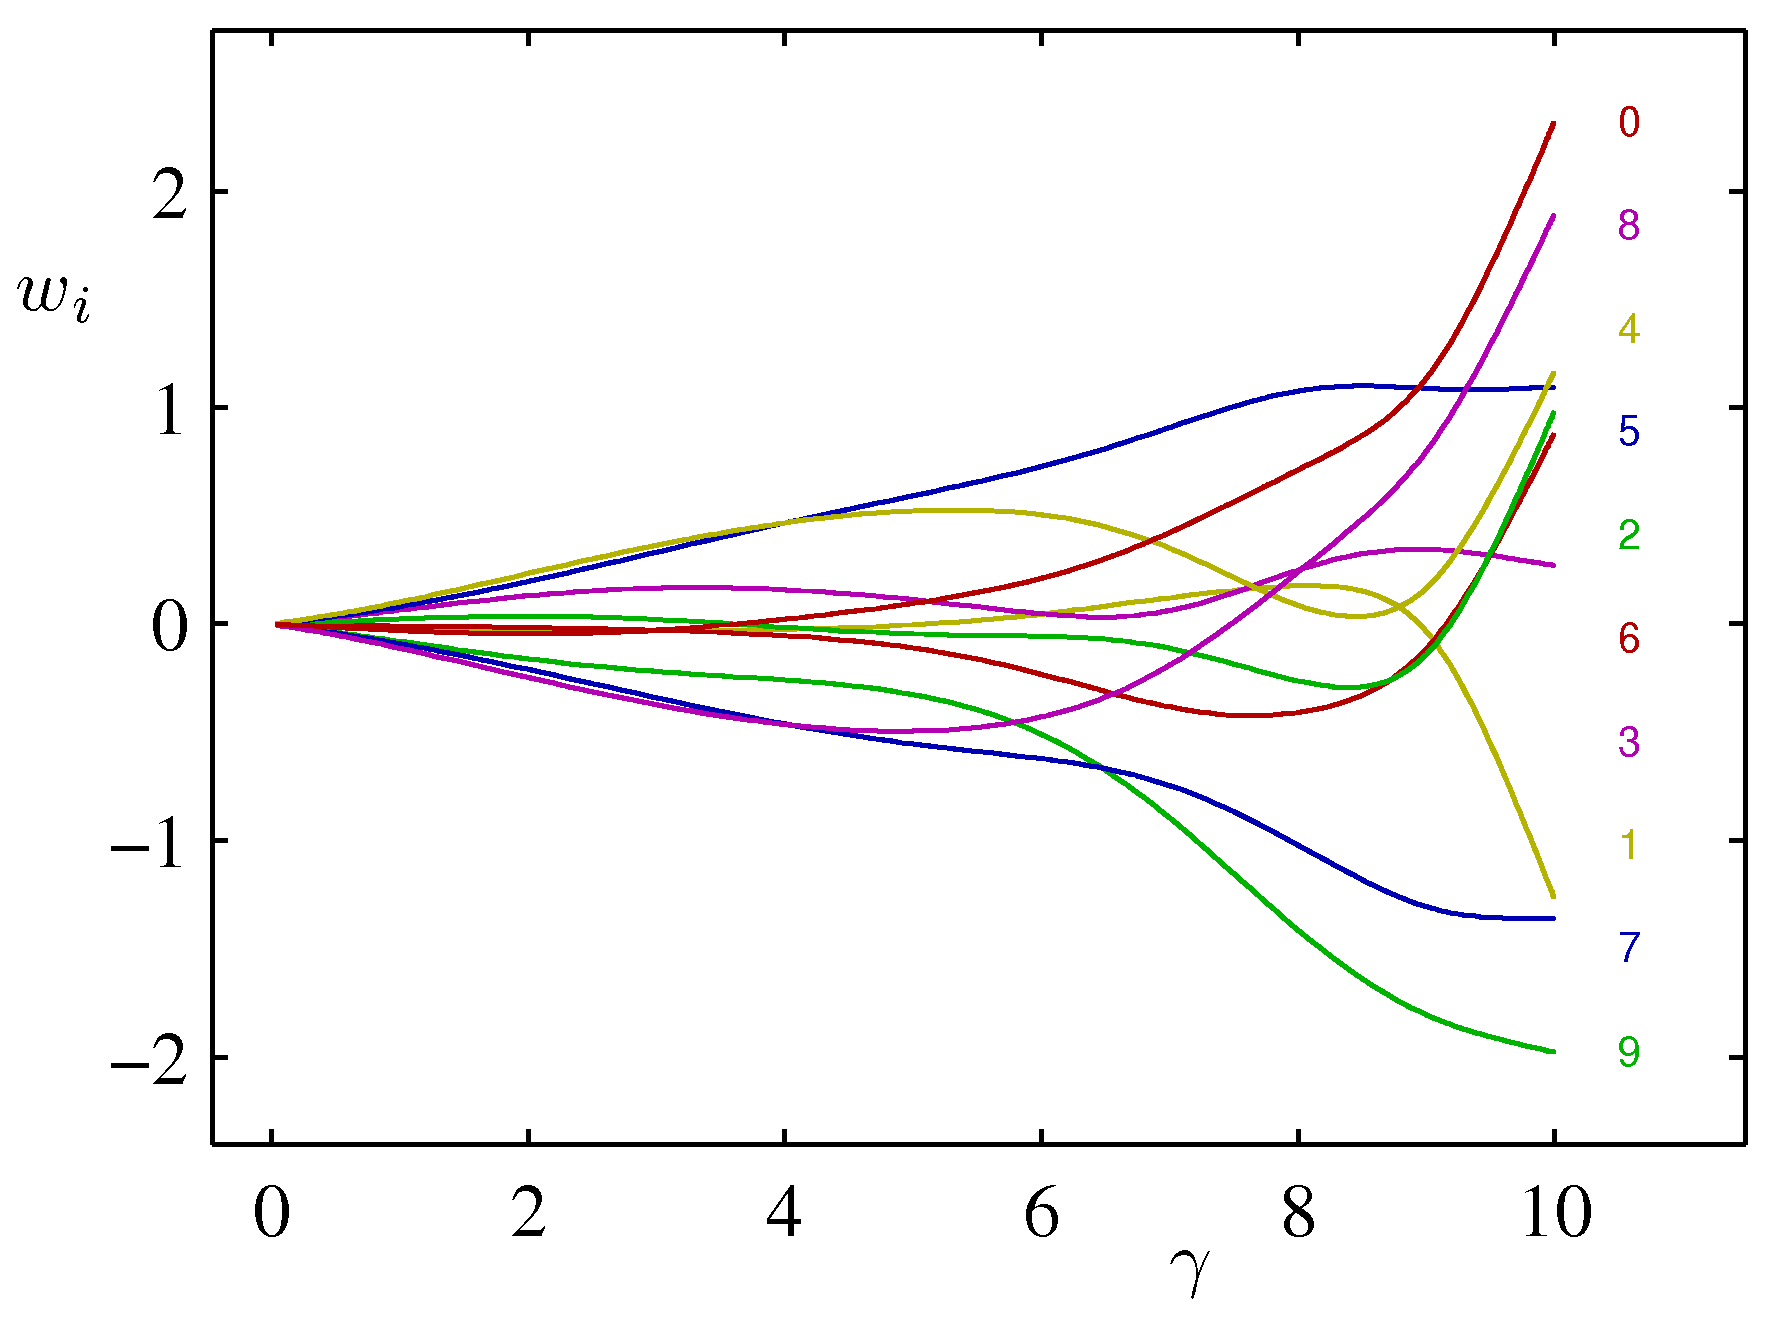
\includegraphics[scale=0.8]{Images/3-17.png}
		\captionsetup{font={small}}
		\caption{高斯基底函数模型中10个参数$w_i$与有效参数数量$\gamma$的关系,其中超参数$0 \leqslant \alpha \leqslant \infty$,于是$\gamma$的范围是$0 \leqslant \gamma \leq M$。}
		\label{fig:3-17}
	\end{figure}
	\\
	\indent 假设一种极端情况$N \gg M$,即数据的数量远大于参数的数量,那么根据(3.87),所有的参数都将是well determined参数,因为$\bfPhi^{\rmT} \bfPhi$包含了所有数据的隐式求和,所以特征值$\lambda_i$会随着数据集规模的增大而增大。在这种情况下,$\gamma = M$,而且$\alpha$和$\beta$的估计方程变成了
	\begin{align}
		\alpha &= \frac{M}{2E_W(\mathbf{m}_N)} \\
		\beta &= \frac{N}{2E_D(\mathbf{m}_N)}
	\end{align}
	其中$E_W$和$E_D$就是(3.25)和(3.26)中所定义的。这些近似结果大幅简化了概率模型重新估计的计算,因为不需要计算Hessian矩阵的特征值了。
	}
	\section{固定基底函数的局限性}
	\insertline\\
	\textnormal{
	\indent 在本章中,我们主要关注的是固定非线性基底函数的线性组合的模型。我们已经看到线性参数具有很多有用的性质,包括最小二乘问题可以求出闭式解,贝叶斯方法也会比较容易使用。此外,为了选择适当的基底函数,我们可以对输入变量到目标变量之间的映射进行任意的非线性建模。在下一章中,我们将研究类似的分类模型。\\
	\indent 由此可见,这样的线性模型似乎是构成了解决模式识别问题的通用框架。然而不幸的是,线性模型存在不少明显的缺点,所以我们需要在后面的章节中研究一些更复杂的模型,比如支持向量机和神经网络等。\\
	\indent 问题究竟出在哪里?主要是因为在得到训练数据集之前就已经假设了基底函数$\phi_j(x)$,而且基底函数一直是固定不变的,这是第1.4节中讨论的维数灾难的表现之一,因为接下来基底函数的数量会随着输入空间的维数$D$呈指数型飞速增长。\\
	\indent 比较走运的是,我们可以利用实际数据集的两个属性来帮助缓解这个问题。首先,由于输入变量之间的强相关性,数据向量$\{x_n\}$通常位于非线性流形内部,其内在维度小于输入空间的维数。在第12章中研究手写数字的图像时,我们会看到这样的例子。如果我们使用局部基底函数,就可以把它们仅分散到输入空间中包含数据的区域内。在使用径向基底函数网络和使用支持向量的相关向量机中会用到这个方法。基于sigmoid非线性自适应基底函数的神经网络模型可以自行调整参数,从而使基底函数在输入空间中的变化与数据流形相对应。第二个属性是目标变量可能仅在数据流形内的少量方向上具有显著的依赖性。神经网络可以通过选择基底函数响应的输入空间中的方向来利用此属性。
	}
\end{document}